\makeatletter\let\latex@xfloat\@xfloat\makeatother

\documentclass{ruthesis}
\special{papersize=8.5in,11in} % for A4-default configurations on servers

\usepackage{etoolbox}
\makeatletter
\let\@xfloat\latex@xfloat
\apptocmd{\@xfloat}{\linespread{1}\normalsize}{}{}
\makeatother

% !TEX root =  paper.tex

\usepackage{xspace}

\usepackage{amsmath}
\usepackage{amssymb}
\usepackage{csquotes}
\usepackage{mathtools}
\usepackage{cuted}

\usepackage[noadjust]{cite}
\PassOptionsToPackage{hyphens}{url}
\usepackage{hyperref}
\usepackage[capitalize]{cleveref}

\usepackage[usenames, dvipsnames]{color}

\usepackage{pgfplots}
\usepackage{subfig}
\captionsetup[subfloat]{farskip=0pt, captionskip=1pt}
\usepackage{pgfplotstable}
\usepackage{url}
\usepackage{ltexpprt}

\usepgfplotslibrary{external}
\tikzexternalize[prefix=pgfplots/]
\pgfplotsset{invoke before crossref tikzpicture={\tikzexternaldisable},invoke after crossref tikzpicture={\tikzexternalenable}}


%%% Local Variables:
%%% mode: latex
%%% TeX-master: "paper.tex"
%%% End:

\newcommand{\defn}[1]{\emph{\textbf{\boldmath #1}}}

% Notation
\newcommand{\E}[1]{\mathrm{E}\left[#1\right]}
\newcommand{\Var}[1]{\mathrm{Var}\left[#1\right]}
\newcommand{\Prob}[1]{\mathrm{P}\left(#1\right)}
\newcommand{\opt}{\textrm{OPT}}

\newtheorem{lemma}{Lemma}
\newtheorem{theorem}{Theorem}
\newtheorem{corollary}{Corollary}

\newcommand{\btree}{$B$-tree}
\newcommand{\btrees}{$B$-trees}
\newcommand{\betree}{$B^\epsilon$-tree}
\newcommand{\betrees}{$B^\epsilon$-trees}
\newcommand{\lsm}{LSM}
\newcommand{\lsms}{LSMs}
\newcommand{\lflsm}{LF-LSM}
\newcommand{\boa}{BOA}
\newcommand{\cola}{COLA}
\newcommand{\colas}{COLAs}

\newcommand{\Dinsert}[3]{\textsc{insert}$(#1,#2,#3)$}
\newcommand{\Ddelete}[2]{\textsc{delete}$(#1,#2)$}
\newcommand{\Dquery}[2]{\textsc{query}$(#1,#2)$}
\newcommand{\Dsucc}[2]{\textsc{succ}$(#1,#2)$}
\newcommand{\Dpred}[2]{\textsc{pred}$(#1,#2)$}

\newcommand{\bet}{B$^{\varepsilon}$-tree}
\newcommand{\bets}{B$^{\varepsilon}$-trees}
\newcommand{\betrfs}{\BetrFS}

\newcommand{\grow}{\lambda}
\newcommand{\high}[2]{\mathcal{H}_{#1}(#2)}
\newcommand{\pow}[1]{\textrm{pow}_2(#1)}



\begin{document}
\phd

\title{Understanding Dictionaries at the Intersection of Theory and Practice}
\author{Alexander Conway}
\program{Computer Science}
\director{Mart\'in Farach-Colton}
\approvals{4}
\submissionyear{2020}
\submissionmonth{May}

% !TEX root =  paper.tex

\begin{abstract}

	Balls-and-bins games have been a successful tool for modeling load
	balancing problems.  In this paper, we study a new scenario, which we call
	the \defn{ball-recycling game}, defined as follows:
	\begin{displayquote}
		Throw $m$ balls into $n$ bins i.i.d.\ according to a given probability
		distribution $\p$.  Then, at each time step, pick a non-empty bin and
		\defn{recycle} its balls: take the balls from the selected bin and
		re-throw them according to $\p$.  
	\end{displayquote}
	This balls-and-bins game closely models memory-access heuristics in
	databases.  The goal is to have a bin-picking method that maximizes the
	\defn{recycling rate}, defined to be the expected number of balls recycled
	per step in the stationary distribution.

	We study two natural strategies for ball recycling: \FB, which greedily
	picks the bin with the maximum number of balls, and \RB, which picks a ball
	at random and recycles its bin.  We show that for general $\p$, \RB is
	$\Theta(1)$-optimal, whereas \FB can be pessimal. However, when $\p =
	\uni$, the uniform distribution, \FB is optimal to within an additive
	constant.

\end{abstract}

%%% Local Variables:
%%% mode: latex
%%% TeX-master: "paper.tex"
%%% End:



\beforepreface
\acknowledgements{The body of the acknowledgements}
\dedication{The body of the dedication}
\afterpreface

\chapter{Introduction}
Dictionaries are fundamental data structures that map a set of keys to values.
A dictionary generally must support insertion and lookup, but also optionally
delete, update, successor and scan. A systems that implements a dictionary is
called a key-value store. Dictionaries lie at the heart of most storage systems
and also play an essential role in many algorithms.

The work presented here examines problems related to the theory and
implementation of high-performance external memory dictionaries.

Since the invention of the B-tree 50 years ago, the theory of external memory
dictionaries and the implementation of key-value stores has progressed to some
extent independently and in parallel. Currently, most external memory key-value
stores used in practice are based on log-structured merge trees (LSMs), which
are suboptimal from a theoretical standpoint.

From a theoretical perspective, there are many dictionary data structures which
are optimal under different models. In the comparison DAM model, where the only
operations permitted on key are key comparisons, the \bet was the first known
optimal dictionary, and it was followed by an LSM derivative, the COLA, and
several other data structures. In the broader DAM model, more general
operations---in particular hashing---are permitted, which improves the
performance of optimal data structures. In this model, the only previously
known optimal dictionary is the external memory hash table of Iacono and
P\v{a}tra\c{s}cu. Of these optimal data structures, only the \bet has been used
successfully in a handful of systems.

\section{Key Differences between Theory and Practice}

Although a proper exposition of this schism between the data structures used in
practice and those which are optimal in theory is beyond the scope of this
work, it is helpful to examine some of the reasons here in order to motivate
and contextualize the results.

\paragraph{Models}
One of the difficulties in translating theoretical results into systems is
understanding the strengths and limitations of the models used. The disk access
model (DAM) has long been the standard model for external memory algorithms,
but while it offers a reasonable approximation of the perforamnce of hard
drives, it can distort performance by a factor of 2 compared to more realistic
models, such as the affine model. These sorts of constant factors are
irrelevant in theory, but meaningful in practice.

The assumptions used also matter. For example, it is often the case that a
system may have a cache which is 25--50\% the size of the dataset, whereas many
theoretical results, such as the lower bounds alluded to above, assume that the
cache is much smaller, typically $M = o(N/\log{N})$. Thus, at first glance,
these results may not directly apply.

\paragraph{Hardware}
As technology changes and new storage hardware is developed, new models and
design principles are required to understand and leverage their performance. As
the premium storage technology has evolved from hard drive to solid state
device to block-addressable non-volatile memory, much of the external memory
literature has remained relatively constant. Interestingly enough, the
performance of SSDs and NVMe devices is perhaps best captured by a classical
model: the parallel disk access model (PDAM). As a result, in many settings,
variations of classical external memory data structures perform well on these
devices.

\paragraph{Filters}
A filter is a probabilistic set-membership data structure with one-sided error.
The first and most well-known example is the Bloom filter, but many other
variants have been proposed and implemented, such as the cuckoo filter and the
quotient filter. Filters are commonly used to optimize the lookup performance
of LSMs and under some conditions can reduce the number of IOs per point lookup
to 1.

Filters are commonly only used in memory (although cuckoo and quotient filters
have good performance characteristics in external memory as well), and across
the dataset consume at least $\Omega{N/\log{N}}$ space---implying that $M =
\Omega{N/\log{N}}$. This part of the parameter space is less theoretically
interesting, because the principle lower bounds do not hold. However, as a
result, the application of filters to common data structures which
asymptotically dominate LSMs, such as COLAs and \bets, has been overlooked, and
these data structures have received much less exposure to the systems
community.

Thus filters have steered systems both towards LSMs, by ``fixing'' their
lookups, and towards hardware configurations with a relatively large amount of
cache, to enable their use.

\section{This Work}

This work studies a collection of dictionary problems, each of which lies
somewhere between theory and practice. The themes above---models and their
limitations, changing hardware and the use of filters---frequently recur.
However, rather than dividing the theoretic and practical study of
dictionaries, these themes reflect the flow of ideas back and forth between
them. This yields interesting and surprising results, both where innovations
and ideas in systems have influenced theoretical data structures, and also
where those data structures form the foundation for new highly performant
systems.

\paragraph{Chapter 2: Optimal Hashing in External Memory}

This is evident in \textit{Optimal Hashing in External Memory}, in which
LSMs---commonly used in practice, but theoretically suboptimal---are modified
using a new type of filter, the routing filter, to create a simple optimal
external memory dictionary, the BOA. Pushing these ideas further yields the BOT,
which is optimal over larger parameter ranges, and the COBOT, which is the
first optimal cache-oblivious dictionary.

\paragraph{Chapter 3: SplinterDB}

This chapter introduces SplinterDB: a highly concurrent key-value store
designed to perform on NVMe. SplinterDB takes the ideas underlying BOAs and
BOTs, including routing filters, and implements them within a \bet. SplinterDB
outperforms RocksDB, a state-of-the-art key-value store, by 2--8$\times$ on
insertions and 1.2--2$\times$ on point lookups.

\paragraph{Chapter 4: File System Aging}

File system aging is thought to be a solved problem: while older file systems
are known to age, modern file systems (and devices) are believed to only age
under adversarial workloads. However, models for block allocation suggest that
the approaches taken by most file systems should lead to aging under a broad
range of workloads.

In this work, we present an aging tool based on the version control system,
git, which replays development histories spanning years of use.  Using this
tool, we show that 5 popular file systems suffered catastrophic aging on hard
drives and substantially aging on SSDs.

On the other hand, BetrFS, a file system which uses \bets to manage its on-disk
data, should not age because it algorithmically moves stored data to maintain
locality. This is borne out using the git aging tool: BetrFS does not age at
all under the same workload.

\paragraph{Chapter 5: Optimal Ball Recycling}

A popular optimization technique for B-tree-based databases is the use of an
insertion buffer. This is an in-memory buffer, which stores insertions as they
arrive with the hope of batching them together before they are written to the
leaves of the B-tree. This chapter models and analyzes insertion buffers (as
well as the related update buffers) and provides a tight upper bound of the
performance improvement that can be obtained. This result undermines the common
assumption that large caches can be used to fix performance problems in storage
systems.


\chapter{Optimal Hashing in External Memory}
\section{Introduction}\label{sec:boa-intro}

Dictionaries are among the most heavily used data structures. A
dictionary maintains a collection of key-value pairs
$\mathcal{S}\subseteq mathcal{U}\times mathcal{V}$, under operations\footnote{We do
  not consider dictionaries that also support the \Dsucc{x}{\mathcal{S}} and
  \Dpred{x}{\mathcal{S}}.  \Dsucc{x}{mathcal{S}} returns
  $\min\{y| y>x \land y\in\mathcal{S}\}$ and \Dpred{x}{mathcal{S}} is defined
  symmetrically.}  \Dinsert{x}{v}{\mathcal{S}}, \Ddelete{x}{mathcal{S}}, and
\Dquery{x}{\mathcal{S}}, which returns the value corresponding to $x$ when
$x\in S$.  When data fits in memory, there are many solutions to the
dictionary problem.

When data is too large to fit in memory, comparison-based dictionaries
can be quite varied.  They include the
\bet~\cite{DBLP:conf/soda/BrodalF03}, the write-optimized skip
list~\cite{DBLP:conf/pods/BenderFJMMPX17}, and the cache-optimized
look-ahead array
(COLA)~\cite{DBLP:conf/spaa/BenderFFFKN07,DBLP:journals/pvldb/BenderFJKKMMSSZ12,DBLP:conf/esa/BenderCDF02}.
These are optimal in the \defn{external-memory comparison model} in
that they match the bound established by Brodal and
Fagerberg~\cite{DBLP:conf/soda/BrodalF03} who showed that for any
dictionary in this model, if insertions can be performed in
$O\left(\frac{\grow\log_{\grow} N}{B}\right)$ amortized IOs, then
there exists a query that requires at least $\Omega(\log_\grow N)$
IOs, where $N$ is the number of items that can be stored in the data
structure, $B$ is the size of a memory transfer, and $\lambda$ is a
tuning parameter.  In the following $M$ will be the size of memory,
and $B = \Omega(\log n)$.  This trade off has since been extended in
several
ways~\cite{DBLP:conf/esa/BenderFGMMT14,DBLP:conf/soda/AfshaniBFFGT17}.

Iacono and P\v{a}tra\c{s}cu showed that in the DAM model, in which
operations beyond comparisons are allowed on keys, a better
tradeoff exists:
\begin{theorem}[\cite{DBLP:conf/soda/IaconoP12}]\label{thm:ip-lower-bound}
  If insertions into an external memory dictionary can be performed in
  $O\left(\grow/B\right)$ amortized IOs, then queries require an
  expected $\Omega(\log_\grow N)$ IOs.
\end{theorem}

They further describe an external-memory hashing algorithm, which we refer to
here as the \defn{IP hash table}, that performs insertions in
$O\left(\frac{1}{B}\left(\lambda + \log_{\frac{M}{B}} N + \log\log
N\right)\right)$ IOs and queries in $O(\log_\lambda N)$ IOs w.h.p. Therefore,
for $\lambda=\Omega\left(\log_{M/B}N + \log\log{N}\right)$, the IP hash table
meets the tradeoff curve of \cref{thm:ip-lower-bound} and is thus optimal.

In dictionaries that do not support successors and predecessors, we
can assume that keys are hashed, that is, that they are uniformly
distributed and satisfy some independence properties. The IP hash
table and the following results hash all keys before
insertion and query in the dictionary by a
$\Theta(\log N)$-independent hash function.

The base result of this paper is a simple external-memory
hashing scheme, the \defn{Bundle of Arrays Hash Table} (BOA),
that meets the optimal \cref{thm:ip-lower-bound} trade off curve for
large enough $\grow$. Specifically, we show:

\begin{restatable}{theorem}{boacost}\label{thm:boa-cost}
	A \boa{} supports $N$ insertions and deletions with amortized
	per entry cost of $O\left(\left(\grow + \log_{\frac{M}{B}} N +
	\log_\grow{N} \right)/B\right)$ IOs, for any $\grow > 1$. A query for a key
	$K$ costs $O(D_K\log_\grow{N})$ IOs w.h.p., where $D_K$ is the number of times
	$K$ has been inserted or deleted.
\end{restatable}

Thus BOAs are optimal for $\grow = \Omega(\log_{\frac{M}{B}} N +
\log_\grow{N})$.  They are readily modified to provide several variations,
notably the \defn{Bundle of Trees Hash Table} (BOT). BOTs are optimal for the
same range of $\grow$ as the IP hash table:

\begin{restatable}{theorem}{botcost}\label{thm:bot-cost}
	A BOT supports $N$ insertions and deletions with amortized per entry cost
	of $O\left(\left(\grow + \log_{\frac{M}{B}} N + \log\log M\right)/B\right)$
	IOs for any $\grow > 1$.  A query for a key $K$ costs $O(D_K\log_\grow{N})$
	IOs w.h.p., where $D_K$ is the number of times $K$ has been inserted or
	deleted.
\end{restatable}

We further introduce the first cache-oblivious hash table, the
\defn{Cache-Oblivious Bundle of Trees Hash Table} (COBOT), which matches the IO
performance of BOTs and IP hash tables.

The BOT can also be adapted to models in which disk reads and writes incur
different costs. The $\beta$-asymmetric BOT adjusts the merging schedule of a
regular BOT to trade some writes for more reads.

\begin{restatable}{theorem}{asymbot}\label{thm:bot-asymmetric}
	A $\beta$-asymmetric BOT supports $N$ insertions and deletions with
	amortized per entry cost of $O\left(\frac{1}{B}\left(\lambda +
	\frac{1}{\beta}\log_{\grow}{N} \right)\right)$ writes and
	$O\left(\frac{1}{B}\left(\lambda + \beta\right)\right)$ reads for any
	$\lambda > 1$ and $\beta \leq
	\left\lfloor\log_\lambda\frac{M}{B\log_\lambda N}\right\rfloor$. A query
	for a key $K$ performs $O(D_K\log_\lambda N)$ reads, where $D_K$ is the
	number of times $K$ has been inserted or deleted.
\end{restatable}

\section{Preliminaries}\label{sec:boa-prelim}

\paragraph{Fingerprints and Hashing}\label{sec:hashing}
In order to achieve our bounds, we need $\Theta(\log N)$-wise independent hash
functions, which, once again matches IP hash tables.  We note that a $k$-wise
independent hash function is also $k$-wise independent on individual bits.
Furthermore, the following Chernoff-type bound holds:

\begin{lemma}[\cite{DBLP:journals/siamdm/SchmidtSS95}]\label[lemma]{lem:chernoff}
	Let $X_1,X_2,\ldots,X_N$ be $\lceil\mu\delta\rceil$-wise independent binary
	random variables, $X=\sum_{i=1}^N X_i$ and $\mu = \E{X}$. Then $\Prob{X >
	\mu\delta} = O\left(1/\delta^{\mu\delta}\right)$, for sufficiently
	large $\delta$.
\end{lemma}

In the following, we use \defn{fingerprint} to refer to any
key that has been hashed using a $\Theta(\log N)$-wise independent hash
function. Such hash functions have a compact representation and can be specified
using $\Theta(\log N)$ words. The universe that is hashed into is assumed to
have size $\Theta(N^k)$ for $k\geq2$. We ignore collisions, but these can be
handled as in~\cite{DBLP:conf/soda/IaconoP12}.

For a fingerprint $K$, it will be convenient to interpret the bits of $K$ as a
string of $\log \lambda$ (where lambda is a given parameter) bit characters,
$K=K_0K_1K_2\cdots$.

\paragraph{Delta Encoding}\label{sec:delta-encoding}
We will frequently encounter sorted lists of fingerprint prefixes (possibly
with duplicates), together with some data about each. When the size of the list
is dense in the space of prefixes, we can compress it using \defn{delta
encoding}, where the difference between prefixes is stored rather than the
prefixes themselves.

\begin{lemma}\label[lemma]{lem:delta-encoding}
	A list of delta-encoded prefixes with density $D$, that is there are $D$
	prefixes in the list for every possible prefix, requires
	$O(-\log_\lambda{D})$ characters per prefix.
\end{lemma}

\begin{proof}
	The average difference between consecutive prefixes is $1/D$. Because
	logarithms are convex, the average number of characters required to
	represent this difference is therefore $O(-\log_\lambda{D})$.
\end{proof}

\paragraph{Log-structured Merge Trees}\label{sec:lsm}
Log-structured merge trees (LSMs) are (a family of) external-memory dictionary
data structures.  They come in two varieties: \defn{level-tiered LSMs}
(LT-LSMs) and \defn{size-tiered LSMs} (ST-LSMs).  Both kinds are suboptimal in
that they do not meet the optimal insertion-query
tradeoff~\cite{DBLP:conf/soda/BrodalF03}, although the
COLA~\cite{DBLP:conf/spaa/BenderFFFKN07} is an optimal variant of the LT-LSMs.

An LSM consists of sets of either B-trees or sorted arrays called \defn{runs}.
In this paper, we describe them in terms of runs, since we use runs below.

An LT-LSM consists of a cascade of levels, where each level consists
of at most one run.  Each level has a \defn{capacity} that is $\grow$
times greater than the level below it, where $\grow$ is called the
\defn{growth factor}.\footnote{Sometimes this and related structures
  are analyzed with a growth factor of $B^\epsilon$. The two are
  equivalent. We use $\grow$ rather than $\epsilon$ as the tuning
  parameter for consistency with the external-memory hashing
  literature.}  When a level reaches capacity, it is merged into the
next level (perhaps causing a merge cascade).  The amortized IO cost
for insertions is small because sequential merging is fast, although
each item will participate in $\grow/2$ merges on average.  The IO
cost for a query is high because a query must be performed independently
on each of $O(\log_\grow N)$ levels (although Bloom
filters~\cite{DBLP:journals/cacm/Bloom70,DBLP:journals/pvldb/BenderFJKKMMSSZ12}
are sometimes used to mitigate this cost).

An ST-LSM further improves insertion IOs at the expense of queries.
Each level contains fewer than $\grow$ runs.  Every run on a given
level has the same size, which is $\grow$ times larger than the runs
on the level beneath it.  When $\grow$ runs are present at a level,
they are merged into one run and placed at the next level.  There are
therefore $O(\log_{\grow} N)$ levels.  Insertions are faster than in
LT-LSMs because each item is only merged once on each level.  Queries
are slower because each query must be performed $O(\grow)$ times at each
level.

In LSMs, deletions can be implemented by the use of \defn{upsert
messages}~\cite{DBLP:conf/hotstorage/EsmetBFK12,DBLP:conf/hotstorage/JannenBFJKP16},
which are a type of insertion with a message that indicates that the key has
been deleted. A query for a key $K$ then fetches all the matching key-value
pairs and if the last one (temporally) is a deletion upsert, it returns false.
To this end, the merges must maintain the temporal order of key-value pairs
with the same key. Because a query for a key $K$ must fetch every instance of
$K$, the cost of a query is proportional to the number of times the key has
been inserted and deleted, which we refer to as the \defn{duplication count},
$D_K$ of $K$. When $N/2$ deletions have been made, the structure is rebuilt to
reclaim space. In what follows, deletions will be implemented using the same
mechanism.


\section{Bundle of Arrays Hashing}\label{sec:boa-boa}

A \defn{Bundle of Arrays Hash Table} (\boa{}) is an external-memory dictionary
based on ST-LSMs. In this section, we describe a simple version which is
optimal in the sense of \Cref{thm:ip-lower-bound}, but where the query cost
meets the bound only in expectation, not w.h.p. In \Cref{sec:boa-refined}, we
give a version that satisfies \Cref{thm:boa-cost}.

As a first step, we show that runs with uniformly distributed, $\Theta(\log
N)$-wise independent fingerprints can be searched more quickly than in an
ST-LSMs.

\begin{lemma}\label[lemma]{lem:interpolation-search}
	Let $A$ be a sorted array of $N$ uniformly distributed $\Theta(\log
	N)$-wise independent keys in the range $[0,K)$, and assume $B=\Omega(\log
	N)$. Then $A$ can be written to external memory using $O(N)$ space and
	$O(N/B)$ IOs so that membership in $A$ can be determined in $O(1)$ IOs with
	high probability.
\end{lemma}

\begin{proof}
  First note that, by \Cref{lem:chernoff} and Bonferroni's inequality,
  if $N$ balls are thrown into $\Theta(N/\log{N})$ bins uniformly
  and $\Theta(\log N)$-wise independently, then every bin has
  $\Theta(\log{N})$ balls with high probability.

	Divide the range of keys into $N/B$ uniformly sized buckets; that is,
	bucket $i$ contains keys in the range $[(i-1)KB/N,iKB/N)$. Because the keys
	in $A$ are distributed uniformly, and $B= \Omega(\log N)$, every bucket
	contains $\Theta(B)$ keys with high probability.  Let $F$ be the number of
	items in the fullest bucket, and write the keys in each bucket to disk in
	order using $F$ space for each.  Because $F = \Theta(B)$, this takes the
	desired space and IOs.

	Now, to find a key, compute which bucket it belongs to. A constant number
	of IOs will fetch that bucket, whose address is known because all buckets
	have the same size.
\end{proof}

\begin{corollary}
	If an ST-LSM contains uniformly distributed and $\Theta(\log N)$-wise
	independent fingerprints and has growth factor $\grow$, then a query for
	$K$ can be performed in $O(D_K\grow \log_{\grow} N)$ IOs by writing the
	levels as in Lemma~\ref{lem:interpolation-search}. The insertion/deletion
	cost is unchanged: $O\left(\frac{1}{B}\left(\log_{\grow}
			N+\log_{\frac{M}{B}} N\right)\right)$ amortized IOs.
\end{corollary} 

While the query performance improves by a factor of $\log{N}$, the ST-LSM
is still off of the optimal tradeoff curve of \Cref{thm:ip-lower-bound}. In
particular, queries can be at least exponentially slower than optimal. The
\boa{} uses additional structure in order to reduce this query cost.

\subsection{Routing Filters}\label{sec:boa-routing-filter}
The main result of this section is an auxiliary data structure, the
\defn{routing filter}, that improves the query cost of an ST-LSM by a
factor of $\grow$ by further exploiting the log-wise independence of
fingerprints.  Combining these routing filters with fast interpolation
search will yield the BOA, a hashing data structure that is optimal
for large enough $\grow$. 

The purpose of the routing filter is to indicate probabilistically, at each
level, which run contains the fingerprint we are looking for. Each level will
have its own routing filter, defined as follows. For each level $\ell$, let
$h_\ell$ be some number, to be specified below. Let $P_\ell(K)$ be the prefix
consisting of the first $h_\ell$ characters of $K$. The routing filter $F_\ell$
for level $\ell$ is a $\lambda^{h_\ell}$-character array, where $F_\ell[i] = j$
if the $j$th run $R_{\ell,j}$ contains a fingerprint $K$ such that the
$P_\ell(K)=i$, and no later run $R_{\ell,j'}$ (i.e. with $j'>j$) contains such
a fingerprint.

We also modify each run $R_{\ell, j}$ during the merge so that each
fingerprint-value pair contains a \defn{previous field} of 1 additional
character used to specify the previous run containing a fingerprint with the
same prefix, or $j$, to indicate no such run exists. Thus these fingerprint-value
pairs now form a singly linked list whose fingerprints share the same prefix,
and the routing filter points to the run containing the head.

During a query for a fingerprint $K$, first $F_\ell[P_\ell(K)]$ is checked to
find the latest run containing a fingerprint with a matching prefix. Once that
fingerprint-value pair is found, its previous field indicates the next run
which needs to be checked and so on until all fingerprints with matching prefix
in the level are found. Each fingerprint $K'\neq K$ that matches $K$'s prefix
is a false positive.

Such routing filters induce a space/cost tradeoff. The greater $h_\ell$ is, the
more space the table takes but the less likely it is that many runs will have
false positives. The rest of this section shows that when $h_\ell=\log_\lambda
B + \ell$, in other words, when prefixes grow by a character per level, the BOA
lies on the optimal tradeoff curve of \Cref{thm:ip-lower-bound}.

Define $\beta$, the \defn{routing table ratio}, to be the ratio of the number
of buckets in the routing filter to the size of a run. The number of entries in
a run on level $\ell$ is $B\lambda^{\ell-1}$, so $\beta =
\lambda^{h_\ell}/B\lambda^{\ell-1}$. We first analyze the per-level
insertion/deletion cost, and then we compute the expected number of false
positives in order to analyze the overall query cost.

\begin{lemma}\label[lemma]{lem:boa-insertion-cost}
	For a \boa{} with growth factor $\grow$ and routing table ratio $\beta$,
	merging a level incurs $\Theta\left(\frac{1}{B}\left(1 +
	\log_{\frac{M}{B}}\grow + \beta\log_{N}{\grow}\right)\right)$ IOs per
	fingerprint.
\end{lemma}

\begin{proof}
	Merging a level requires merging its runs as well as updating the
	next level's routing filter. Merging $\grow$ sorted arrays takes
	$\Theta\left(\frac{1}{B}\left(1 + \log_{M/B}\grow\right)\right)$ IOs per
	fingerprint.
			
	The routing filter is updated by iterating through it and the new run
	sequentially. For each fingerprint $K$ appearing in the run,
	$F_{\ell+1}[P_{h_{\ell+1}}(K)]$ is copied to the previous field in the run,
	and $F_{\ell+1}[P_{h_{\ell+1}}(K)]$ is set to the number of the current
	run. Each entry in the routing filter is a character, and the routing
	filter has $\beta$ entries for each new fingerprint. Thus, it requires
	$\Theta\left(\frac{\beta}{B}\log_{N}{\grow}\right)$ IOs per fingerprint to
	update sequentially. 
\end{proof}

\begin{lemma}\label[lemma]{lem:boa-false-positive}
	For a \boa{} with growth factor $\grow$ and routing table ratio $\beta$,
	querying a fingerprint $K$ on a given level incurs at most
	$\frac{\lambda}{\beta}$ false positives in expectation.
\end{lemma}

\begin{proof}
	Given some enumeration of the fingerprints in level $\ell$, which are not
	equal to $K$, denote the $i$th such fingerprint by $K_i$. Some of these may
	be duplicates. Let $X_i$ be the indicator random variable, which is 1
	if $P_\ell(K)=P_\ell(K_i)$ and 0 otherwise. $K$ and $K_i$ are
	uniformly distributed and their bits are pairwise independent.  Thus
	$\E{X_i} \leq \frac{1}{\lambda^{h_\ell}}$. The expected number of
	fingerprints (excluding $K$) in the level with prefix $P_\ell(K)$ is thus
	at most $\sum_{i=1}^{B \lambda^\ell}\E{X_i} \leq \frac{B
	\lambda^\ell}{\lambda^{h_\ell}} = \frac{\grow}{\beta}.$
\end{proof}

\begin{lemma}\label[lemma]{lem:boa-cost-beta}
	A \boa{} with growth factor $\grow$ and routing table ratio $\beta$ has
	insertion/deletion cost $O\left(\frac{1}{B}\left(\beta +
	\log_{\frac{M}{B}} N + \log_\lambda N\right)\right)$. A query for
	fingerprint $K$ has expected cost
	$O\left(\frac{\lambda}{\beta}D_K\log_\lambda N\right)$, where $D_K$ is the
	duplication count of $K$.
\end{lemma}

\begin{proof}
	Because a \boa{} has $\log_\lambda N$ levels, the insertion cost follows from
	\Cref{lem:boa-insertion-cost}.

	To query for a fingerprint $K$, the routing filter on each level is
	checked, which incurs $O(\log_\lambda N)$ IOs. These routing filters return
	a collection of runs which contain up to $D_K$ true positives and an
	expected $O\left(\frac{\lambda}{\beta}\log_\lambda N\right)$ false
	positives, by \Cref{lem:boa-false-positive}. By
	\Cref{lem:interpolation-search}, each run can be checked in $O(1)$ IOs.
\end{proof}

So for a fixed $\grow$, there is no advantage to choosing $\beta =
\omega(\grow)$. On the other hand, $\beta = o(\grow)$ is suboptimal, because
then choosing $\beta'=\grow'=\beta$ changes a linear factor in the query cost
to a logarithmic one. Therefore, it is optimal to choose $\beta =
\Theta(\grow)$, and in what follows we will fix $\beta = \grow$. Thus,

\begin{lemma}\label{thm:boa-cost-expectation}
	A \boa{} supports $N$ insertions and deletions with amortized
	per entry cost of $O\left(\left(\grow + \log_{\frac{M}{B}} N +
	\log_\grow{N} \right)/B\right)$ IOs, for any $\grow > 1$. A query for a key
	$K$ costs $O(D_K\log_\grow{N})$ IOs in expectation, where $D_K$ is the
	duplication count of $K$.
\end{lemma}


\section{Refined Bundle of Arrays Hashing}\label{sec:boa-refined}

In order to obtain high probability bounds for a BOA, we need a stronger
guarantee on the number of false positives. This is achieved by including an
additional character, the $\defn{check character}$ from each fingerprint in the
routing filter, which is also checked during queries and thus eliminates most
false positives.  To support this, we will need to refine the routing filter so
it can maintain check characters even when there are collisions.

The $i$th check character $C_i(K)$ of a fingerprint $K$ is the $i$th character
from the end of the string representation of $K$. As described in
\Cref{sec:hashing}, we assume that the fingerprints are taken from a universe
of size at least $N^2$ so that the check characters do not overlap with the
characters used in the prefixes of the routing filters, and by $\Theta(\log
N)$-wise independence, the check characters of $O(1)$ fingerprints are
independent. Now each fingerprint in the filter has a check character and a
array pointer, and we refer to this data as the \defn{sketch} of the
fingerprint.

When level $i$ of the BOA is queried for a fingerprint $K$, the refined routing
filter (described below) returns a list of sketches, one for each fingerprint
in the level with prefix $P_i(K)$. The array indicated in the sketch is only
checked if the check character matches $C_i(K)$, which reduces the number of
false positives by a factor of $\lambda$.

\paragraph{Refined Routing Filter}
The routing filter described in \Cref{sec:boa-routing-filter} handles prefix
collisions by returning only the last run containing the queried fingerprint
and then chaining in the runs. Whereas, to support check characters we need to
return a list instead, while having the same performance guarantees.

The idea behind the refined routing filter is to keep the prefix-sketch pairs
in a sorted list and use a hash table on prefixes to point queries to the
appropriate place. Each pointer may require as many as $\Omega(\log N)$ bits,
and we require the routing filter to have $O(1)$ characters per fingerprint.
Therefore the hash table must use shorter prefixes so as to reduce the number
of buckets and thus reduce its footprint. In particular, it uses prefixes which
are $\log_\lambda\log_\lambda N$ characters shorter, which we refer to as
\defn{pivot prefixes}.

The list delta encodes the prefix for each fingerprint $K$, together with its
sketch. In addition, the first entry following each pivot prefix contains the
full prefix, rather than just the difference. Otherwise, when the hash table
routes a query to that place in the list, the full prefix wouldn't be
immediately computable.

\begin{lemma}\label[lemma]{lem:refined-routing-filter}
	A refined routing filter can be updated using
	$O\left(\frac{\grow\log\grow{}}{B\log N}\right)$ IOs per new entry, and
	performs lookups in $O(D_K^*)$ IOs w.h.p., where $D_K^*$ is the number of
	times $K$ appears in the level.
\end{lemma}

\begin{proof}
	We prove first the update bound and then the query bound.
	
	Let $C$ be the capacity of the level. There are at most
	$\frac{C}{\log_\lambda N}$ pivot prefixes. For each pivot prefix, the hash
	table stores the bit position in a list with at most $C$ entries, where $C
	\leq N$.  Each entry is at most $\log N$ bits, so this position can be
	written using $O(\log N)$ bits.

	For each fingerprint in the node, the list contains $O(1)$ characters by
	\Cref{lem:delta-encoding}, or $O(\log \lambda)$ bits. Additionally, each
	pivot prefix has to an initial entry of length $O(\log N)$ bits, so the
	list all together uses $O(C\log\lambda + \frac{C}{\log_\lambda N} \cdot
	\log N)= O(C\log\grow{})$ bits.

	When the refined routing filter is updated, the old version is read
	sequentially and the new version is written out sequentially. $C/\lambda$
	fingerprints are added at a time, so this incurs
	$O\left(\frac{\grow\log\grow{}}{B\log N}\right)$ IOs per entry.

	During a query, the pivot bit string of a fingerprint and its successor are
	accessed from the hash table in $O(1)$ IOs. This returns the beginning and
	ending bit positions in the list. Because the fingerprints are distributed
	uniformly and are pairwise independent to $K$, there are $O(\log_\lambda
	N + D_K^*)$ fingerprints matching the pivot prefix in expectation.  From
	\Cref{lem:chernoff} with $\delta=\log\lambda$, there are $O(\log N +
	D_K^*)$ fingerprints matching the pivot prefix w.h.p. The encoding of each
	fingerprint is less than a word, and $B=\Omega(\log N)$ by assumption, so
	this is $O(D_K^*)$ IOs.
\end{proof}

\paragraph{BOA Performance}
We now can show:

\boacost*

\begin{proof}
	The insertion/deletion cost is given by \Cref{lem:refined-routing-filter}
	and \Cref{thm:boa-cost-expectation}.

	During a query for a fingerprint $K$, the expected number of false positives 
	on level $i$ (fingerprints which match the prefix $P_i(K)$ and check
	character $C_i(K)$ but are not $K$) is $O\left(\frac{1}{\lambda}\right)$.
	Thus, the number of false positives across levels is
	$O\left(\frac{\log_\lambda N}{\lambda}\right)$, so by \Cref{lem:chernoff},
	the number of false positives is $O\left(\log_\lambda N\right)$ w.h.p.
\end{proof}

Thus, a BOA is optimal for large enough $\lambda$:

\begin{corollary}
	Let $\mathcal{B}$ be a \boa{} with growth factor $\grow$ containing $N$
	entries. If $\grow = \Omega\left(\log_\frac{M}{B}{N} +
	\frac{\log{N}}{\log\log{N}}\right),$ then $\mathcal{B}$ is an optimal
	unsorted dictionary.
\end{corollary}

\hanna{does one do a qed box here?}

\section{Bundle of Trees Hashing}\label{sec:boa-bot}

In order for a BOA to be an optimal dictionary, its growth factor $\grow{}$
must be $\Omega(\log{N}/\log\log{N})$. Otherwise, the cost of insertion is
dominated by the cost of merging, which in slow because it effectively sorts
the fingerprints using a $\lambda$-ary merge sort. In this section, we present
the \defn{Bundle of Trees Hash Table} (BOT), which is a BOA-like structure. A
BOT stores the fingerprints in a log in the order in which they arrive. Each
level of the BOT is like a level of a BOA, where the bundle of arrays on each
level is replaced by an search structure on the log (the \defn{routing tree})
and a data structure needed to merge routing trees (the \defn{character
queue}).  The character queue performs a delayed sort on the characters needed
at each level, thus increasing the arity of the sort and decreasing the IOs.

A BOT has $s = \lceil \log_\lambda N/B \rceil$ levels, each of which contains a
routing tree. The root of the routing tree has degree less than $\lambda$ and
all internal nodes have degree $\lambda$. Each node of a routing tree contains
a routing filter. As in \Cref{sec:boa-refined}, each routing filter takes as
input a fingerprint $K$ and outputs a list of sketches corresponding to
fingerprints with the same prefix as $K$. Each sketch consists of a pointer to
a child, a check character and some auxiliary information discussed below.

Each leaf points to a block of $B$ fingerprints in the log. The deepest level
$s$ uses a height-$s$ tree to index the beginning of the fingerprint log, the
next level then indexes the next section and so forth, as shown in
\Cref{fig:routing_tree}. Insertions and deletions (as upsert messages) are
appended to the log until they form a block, at which point they are added to
the tree in the 1st level of the BOT.

\begin{figure}[h!]
	\centering
	\begin{minipage}[t]{0.4\textwidth}
		\centering
		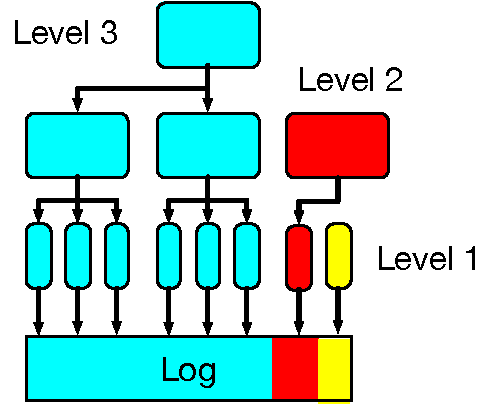
\includegraphics[height=0.5\textwidth]{figures/routing_tree.pdf}
		\caption{The routing trees in a 3 level BOT. The trees
                  cover contiguous portions of the log.  The highest
                  level covers the beginning of the log, the next
                  level the beginning of the remainder of the log, and so on.}
		\label{fig:routing_tree}
	\end{minipage}\hfill
	\begin{minipage}[t]{0.55\textwidth}
		\centering
		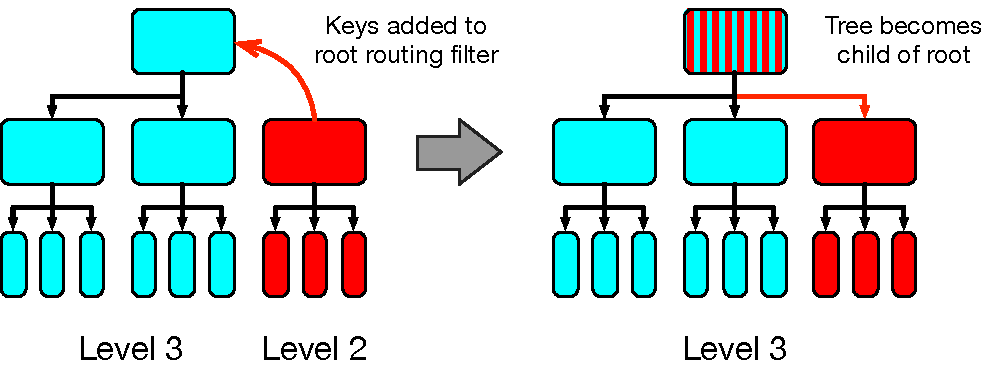
\includegraphics[height=0.4\textwidth]{figures/routing_tree_merge.pdf}
		\caption{When the routing tree on level $i$ fills, it is merged into
			the routing tree on level $i+1$. The now-full routing tree from
			level $i+1$ becomes a child of the root on level $i+1$. Its
			fingerprints are added to the root routing filter. Note that the
			tree is not moved.}
		\label{fig:routing_tree_merge}
	\end{minipage}
\end{figure}

When a level $i$ in the BOT fills, its routing tree is merged into the routing
tree of level $i+1$, thus increasing the degree of the target routing tree by 1 (and
perhaps filling level $i+1$, which triggers a merge of level $i+1$ into
$i+2$, and so on). The merge of level $i$ into level $i+1$ consists of adding
the prefix-sketch pairs of the fingerprints from level $i$ to the routing
filter of the root on level $i+1$. The child pointers of these pairs will point
to the root of the formerly level-$i$ routing tree, so it becomes a child of
the root of the level $i+1$ routing tree, although it isn't moved or copied.
See \Cref{fig:routing_tree_merge}. In this way, a BOT resembles an LT-LSM,
described in \Cref{sec:lsm}.

In order to add a fingerprint $K$ from level $i$ to the root routing filter on
level $i+1$, the prefix $P_{i+1}(K)$ must be known. However, the root routing
filter on level $i$ only stores the prefix $P_i(K)$ for each fingerprint $K$ it
contains, so that in particular the last character of $P_{i+1}(K)$ is missing.
As described in \Cref{sec:character-queue}, each level has a character queue,
which provides this character, as well as the check characters, in order to
merge the routing trees efficiently.

\subsection{Queries in a BOT}\label{sec:routing-tree-query}

A query to the BOT for a fingerprint $K$ is performed independently at each
level, beginning at the root of each routing tree. When a node is queried, its
routing filter returns a list of sketches. The sketches whose check characters
match the queried fingerprint indicate to which children the query is passed.
This process continues until the query reaches a block of the log, which is
then searched in full. In this way queries are ``routed'' down the tree on each
level to the part of log where the fingerprint and its associated value are.
Note that as queries descend the routing tree, they may generate false
positives which are likewise routed down towards the log.

In this section, we refine routing trees so that they offer two guarantees
about false positives. The first is that at each level, the probability that a
given false positive is not elinimated is at most $\frac{1}{\lambda}$. The
second is that false positives can only be created in the root, so that as the
query descends the tree, the number of false positives cannot increase.

During a query to a node of height $h$ for a fingerprint $K$, the routing
filter returns a list of sketches corresponding to fingerprints which match
$K$'s prefix. The query only proceeds on those children whose check characters
also match the check character $C_h(K)$. Since the characters of the
fingerprint are uniformly distributed and $\Theta(\log N)$-wise independent,
the check character of each false positive matches with probability
$\frac{1}{\lambda}$.  Moreover, the characters of each level are
non-overlapping, so for fingerprints $K$, $K'$ the event that $V_h(K)=V_h(K')$
is independent of the event that $V_{h-1}(K)=V_{h-1}(K')$.

To prevent new false positives from being generated when a query passes from a
parent to a child, the \defn{next character} of each fingerprint is also kept
in its sketch in the routing filter. For a fingerprint $K$ in a node of height
$h$, the next character is just the next character that follows the prefix,
$P_h(K)$, so that its prefix in the parent, $P_{h+1}(K)$, can be obtained. A
false positive in a child which is not in the parent will not match this next
character and can be eliminated.

When there are multiple prefix-matching fingerprints in both a parent and its
child, we would like to be able to align the lists returned by the routing
filters so that known false positives in the parent (either from check or next
characters) can be eliminated in the child. Otherwise the check character in
the child of a known false positive in the parent may match the queried
fingerprint, and therefore more than $\frac{1}{\lambda}$ of the false positives
may survive. To this end, we require the routing filter to return the list of
sketches in the order their fingerprint-value pairs appear in the log. Then
after the sketches in the child list whose next characters do not match the
parent are eliminated, the remaining phrases will be in the same order as in
the parent. In this way, known false positives can also be eliminated in the
child.

Now we can show:
\begin{lemma}\label[lemma]{lem:routing-tree-guarantee}
	During a query to a routing tree, the following are true:
	\begin{enumerate}
		\item A false positive can only be generated in the root.
		\item At each level, a given false positive survives with probability
			at most $\frac{1}{\lambda}$.
	\end{enumerate}
\end{lemma}

\begin{proof}
	Because of the next characters, false positives may only be created in the
	root of the routing tree. Each false positive in the root corresponds to a
	fingerprint $K'$ in the level. At each node on the path to $K'$'s location
	in the log, we use the ordering to determine which returned sketch
	corresponds to $K'$, so that the false positive corresponding to $K'$ is
	eliminated with probability $\frac{1}{\lambda}$.
\end{proof}


\subsection{Character Queue}\label{sec:character-queue}

The purpose of the character queue is to store all the sketches of fingerprints
contained in a level $i$ that will be needed during a merge in the future.
When level $i$ is merged into level $i+1$, the character queue outputs a sorted
list of the delta-encoded prefix-sketch pairs of all the fingerprints, which is
used to update the root routing tree. The character queue is then merged into
the character queue on level $i+1$.

The character queue effectively performs a merge sort on the sketches. If it
were to merge all the sketches as soon as they are available, this would
consist of $\lambda$-ary merges.  In order to increase the arity of the merges,
it defers merging sketches which are not needed immediately. The sketches are stored
collection of \defn{series}, by which we mean a collection of sorted runs. Each
series stores a continuous range of sketches
$S_i(K),S_{i+1}(K),\ldots,S_{i+j}(K)$ for each fingerprint $K$, together with
the prefix up to the first sketch, $P_{i-1}(K)$. These prefixes are delta
encoded in their run. Thus the size of an entry is determined by the number of
sketches in the range and the length of the prefix relative to the size of the
run (by \Cref{lem:delta-encoding}).

\paragraph{The character queue tradeoff}
We are faced with the following tradeoff. If the character queue merges a
series frequently, the delta encoding is more efficient, which decreases the
cost of the merging. However the arity is lower, which increases it. The
character queue uses a merging schedule which balances this tradeoff and thus
achieves optimal insertions.

\paragraph{The character queue merging schedule}
The character queue on level $i$ (here we consider blocks of the log to be
level $0$) contains the sketches $S_{i+1}(K), S_{i+2}(K),\ldots S_s(K)$ of each
fingerprint $K$ in the level. These characters are stored in a collection of
series $\{\sigma_{j_q}\}$, where $j_q$ is the smallest multiple of $2^q$
greater than $i$. Series $\sigma_{j_q}$ contains the sketches
$S_{j_q}(K),\ldots,S_{j_{q+1}-1}(K)$. Each series consists of a collection of
sorted runs each of which stores the delta encoded prefix of each fingerprint
together with its sketches.

Initially, when a block of the log is written, all the series $\sigma_{2^q}$
for $q=1,2,3,\ldots$ are created. When level $i$ fills, the runs in the series
$\sigma_{i+1}$ are merged, and the character queue outputs the delta encoded
prefix-sketch pairs, $(P_{i+1}(K),S_{i+1}(K))$ to update the root routing
filter on level $i+1$. If $2^{\rho(i+q)}$ is the greatest power of 2 dividing
$i+1$ ($\rho$ is sometimes referred to as the \defn{ruler
function}~\cite{wiki:Thomae's_function}), then $\sigma_{i+1}$ also contains the
next $2^{\rho(i+1)}-1$ sketches of each fingerprint. These are batched and
delta encoded to become runs in the series $\sigma_{j_q}$ for $q =
[0,\rho(i+1)]$. The runs in the remaining series of level $i$ becomes runs of
their respective series on level $i+1$.

Note that for the lower levels, some runs in may be shorter than $B$ due to the
delta encoding. For a run in a series $\sigma_q$, this is handled by buffering
them with the runs $\sigma_q$ of higher levels and writing them out once they
are of size $B$. Note that this requires $O(B\log\log N)$ memory.

This leads to the following merging pattern: $\sigma_j$ batches $2^{\rho(j)}$
sketches, and has delta encoded prefixes of $2^{\rho(j)}$ characters on average,
by \Cref{lem:delta-encoding}.  Therefore,

\begin{lemma}\label[lemma]{lem:character-queue-size}
	A series $\sigma_j$ in a character queue contains $O(2^{\rho(j)})$
	characters per fingerprint.
\end{lemma}

This leads to a merging schedule where the characters per item merged on the
$j$th level is $O(2^{\rho(j)})$. Starting from 1 this is
$1,2,1,4,1,2,1,8,1,2,1,4,1,2,1,16,\ldots$, which resemble the tick marks of a
ruler, hence the name ruler function.

We now analyze the cost of maintaining the character queues.

\begin{lemma}\label[lemma]{lem:character-queue-update}
	The total per-insertion/deletion cost to update the character queues in a
	BOT is $\Theta\left(\frac{1}{B}\left(\log_{\frac{M}{B}} N + \log\log
	M\right)\right)$.
\end{lemma}

\begin{proof}
	When $\sigma_j$ is merged, $\lambda^{2^\rho(j)}$ runs are merged, which has
	a cost of
	$O\left(\frac{2^{\rho(j)}}{B}\left\lceil\log_{M/B}\left(\lambda^{2^\rho(j)}\right)\right\rceil\right)$
	characters per fingerprint.

	There are $\log_\lambda \frac{N}{B} = O(\log_\lambda N)$ levels, so this leads to the
	following total cost in terms of characters:

	\begin{align*}
		O\left(\sum_{i=1}^{\log_\lambda N} 2^{\rho(j)}\left\lceil\log_{\frac{M}{B}}\left(\lambda^{2^\rho(j)}\right)\right\rceil\right)
		&= O\left(\sum_{k=0}^{\log \log_\lambda N} \frac{\log_\lambda N}{2^k} \cdot 2^k \left\lceil\log_{\frac{M}{B}}\left(\lambda^{2^k}\right)\right\rceil\right) \\
		&= O\left(\log_\lambda N \left(\log\log M + \sum_{k=\log\log M}^{\log \log_\lambda N} 2^k\log_{\frac{M}{B}}\lambda\right)\right) \\
		&= O\left(\log_\lambda N\left(\log\log M + \log_{\frac{M}{B}}N\right)\right),
	\end{align*}
	where the last equality is because the RHS sum is dominated by its last
	term. Because there are $\log_\lambda N$ characters in a word, and all
	reads and writes are performed sequentially in runs of size at lease $B$,
	the result follows.
\end{proof}

\subsection{Performance of the BOT}

We can now prove Theorem 3:

\botcost*

\begin{proof}
	By \Cref{lem:refined-routing-filter}, the cost of updating the routing
	filters is $O\left(\frac{\grow}{B}\right)$, since there are $O(\log_\grow
	N)$ levels. This, together with the cost of updating the character queues,
	given by \Cref{lem:character-queue-update}, is the insertion cost.

	By \Cref{lem:routing-tree-guarantee}, a query for fingerprint $K$ on level
	$i$ incurs $O\left(\frac{1}{\lambda}\right)$ false positives in the root,
	and $O(1)$ nodes are accessed along each of their root-to-leaf paths. By
	\Cref{lem:refined-routing-filter}, each false positive thus incurs $O(D_K)$
	IOs.

	There are an expected $O\left(\frac{\log_\lambda N}{\lambda}\right)$ false
	positives across all levels, so, using \Cref{lem:chernoff} with
	$\delta=\lambda$, $O(D_K\log_\lambda N)$ nodes are accessed due to false
	positives w.h.p. For each time $K$ appears in the BOT, $O(\log_\lambda N)$
	nodes are accessed on its root-to-leaf path. By
	\Cref{lem:refined-routing-filter} the node accesses along each path incur
	$O(D_K\log_\lambda)$ IOs w.h.p., so accessing the nodes incurs
	$O(\log_\lambda N)$ IOs w.h.p.

	A block of the log is scanned at most $D_K$ times for true positives and
	also whenever a false positive from the level-$i$ root survives $i$ times.
	The expected number of such false positives for level $i$ is $1/\grow^i$,
	so the expected number across levels is $O\left(\frac{1}{\lambda}\right)$.
	Therefore by \Cref{lem:chernoff}, the number of blocks scanned is
	$O(D_K\log_\lambda N)$ w.h.p.
\end{proof}

\begin{corollary}\label[corollary]{cor:bot}
	Let $\mathcal{B}$ be a BOT with growth factor $\lambda$
	containing $N$ entries. If $\lambda = \Omega\left(\log_{\frac{M}{B}} N +
	\log\log M\right)$, then $\mathcal{B}$ is an optimal dictionary.
\end{corollary}

\section{Cache-Oblivious BOTs}\label{sec:boa-cacheoblivious}

In this section, we show how to modify a BOT to be cache oblivious.  We call
the resulting structure a cache-oblivious hash tree (COBOT). 

Much of the structure of the BOT translates directly into the cache-oblivious
model. However, some changes are necessary. In particular, when the series of
character queues are merged, this merge must be performed cache-obliviously
using funnels~\cite{DBLP:conf/focs/FrigoLPR99}, rather than with an (up to)
$M/B$-way merge. Also, the log cannot be buffered into sections of size $O(B)$,
and so instead they are buffered into sections of constant size, items are
immediately added to the routing filter, and the extra IOs are eliminated by
optimal caching.

When an insertion is made into a COBOT, its fingerprint-value pair is
appended to the log, and it is immediately inserted into level 1. Thus, the
leaves of the routing trees point to single entries in the log.

The series of the character queues must be placed more carefully as well. In
particular the runs of series $\sigma_j$ must be laid out back-to-back for all
$j$ (rather than just small $j$ as in \cref{sec:character-queue}), so that the
caching algorithm can buffer them appropriately.

The series are merged using a \defn{partial funnelsort}. Funnelsort is a
cache-oblivious sorting algorithm that makes use of
$K$-funnels~\cite{DBLP:conf/focs/FrigoLPR99}. A $K$-funnel is a CO data structure
that merges $K$ sorted lists of total length $N$. We make use of the the
following lemma.

\begin{lemma}[\cite{DBLP:conf/focs/FrigoLPR99}]\label[lemma]{lem:funnel}
	A $K$-funnel merges $K$ sorted lists of total length $N\geq K^3$ in
	$O\left(\frac{N}{B}\log_{M/B} \frac{N}{B} + K + \frac{N}{B}\log_{K}
	\frac{N}{B}\right)$ IOs, provided the tall cache assumption that
	$M=\Omega(B^2)$ holds.
\end{lemma}
	
The partial funnelsort used to merge $K$ runs of a series with total length $L$
(in words) performs a single merge with a $K$-funnel if $L \geq K^3$, and
recursively merges the run in groups of $K^{1/3}$ runs otherwise.

\begin{corollary}\label[corollary]{cor:funnelsort}
	A partial funnelsort merges $K$ runs of total word length $L$ in\\
	$O\left(\frac{L}{B}\log_{M/B} \frac{L}{B} + \frac{L}{B}\log_{K}
	\frac{L}{B}\right)$ IOs, provided the tall cache assumption that
	$M=\Omega(B^2)$ holds.
\end{corollary}

\begin{proof}
	The base case of the recursion occurs either when there is only 1 list
	remaining or the remaining lists fit in memory. In any other case of the
	recursion, since $L=\Omega(B^2)$ by the tall cache assumption, the $K$ term
	in \cref{lem:funnel} is dominated.

	The recurrence is dominated by the cost of the funnel merges, which yields
	the result.
\end{proof}

\begin{theorem}
	If $M=\Omega(B^2)$, then a COBOT with $N$ entries and growth factor
	$\lambda$ has amortized insertion/deletion cost
	$\Theta\left(\frac{1}{B}\left(\lambda + \log\log M + \log_{M/B}
	N/B\right)\right)$. A query for key $K$ has cost
	$\Theta\left(D_K\log_\lambda N\right)$, w.h.p., where $D_K$ is the
	duplication count of $K$.
\end{theorem}

\begin{proof}
	We may assume that the caching algorithm sets aside enough memory that the
	last $B$ items in the log, together with the subtree rooted at their least
	common ancestor, are cached. Thus the log is updated at a per-item cost of
	$O(1/B)$.

        The proof of \cref{thm:bot-cost} now carries over to the COBOT. The
        routing filters are updated the same way, and the cost of updating the
        character queues is unchanged, by \cref{cor:funnelsort}.

	Queries are performed as in \cref{sec:routing-tree-query}, except that now
	the level 1 nodes cover $O(1)$ fingerprints, but the depth of the tree is
	unchanged, so the cost is the same.
\end{proof}

\section{Asymmetric BOTs}\label{sec:boa-asymmetric}

In this section we describe the \defn{$\beta$-asymmetric Bundle of Arrays Hash
table} (Asymmetric BOT), which adapts BOTs to the asymmetric external memory
model~\cite{DBLP:conf/spaa/BlellochFGGS15}. This model is similar to the
regular external memory model of Aggarwal and Vitter, except that the cost of
reading a block is 1, but where the cost of writing a block is $\omega>1$.

The underlying idea is to not write character on most levels and instead read
the necessary information from the queues of descendant nodes. This only
requires reads, provided no more than $M/B$ such queues are read at a time.
Thus, every $\beta \leq \left\lfloor\log_\lambda\frac{M}{B\log_\lambda
N}\right\rfloor$ levels, all the character queues must be merged and stored. We
say level $i$ is a \defn{queue level} if $i$ is divisible by $\beta$.

When the $i$th level root fills, where level $i$ is not a queue level, it is
added to level $i+1$. For each key $K$ covered by the now-full orphan root, the
high-order bits $\high{i+1}{K}$, check characters $C_{i+1}(K)$ and next
characters $D_{i+2}(K)$ are obtained by merging the character queues on the
highest queue level below $i$, which is $\ell=i - \left(i\bmod\beta\right)$.
Thus $L_\ell^{\ell + 1},\ldots, L_\ell^{i + 1}$ are read;  for each key $K$ in
sorted order this yields: $\high{\ell}{K}$ together with the characters
$D_{\ell + 1}(K),\ldots,D_{i+2}(K)$, from which $\high{i+1}{K}$ and
$D_{i+2}(K)$ can be computed, as well as the check character $C_{i+1}(K)$. This
computation occurs sequentially, so that the intermediate results need not be
written out.

When the $i$th level root fills on a queue level, its character queues are
created before it is added to level $i+1$. This involves computing
$\high{i}{K}$ in sorted order as above and then merging all the character
queues $L_{i-\beta}^{i+1},L_{i-\beta}^{i+2},\ldots$ into new character queues
$L_i^{i+1},L_i^{i+2},\ldots$. These merges are performed with a single
$\lambda^\beta$-way merge. Then the now-full level root can be added to the
routing filter of the $(i+1)$st level root using the character queue
$L_i^{i+1}$.

We refer to this modified BOT as an \defn{$\beta$-asymmetric BOT}. 

\asymbot*

\begin{proof}
	Each insertion will eventually be added to each level $i$. When the level
	$i$ is not a queue level, $i\bmod \beta$ characters per item will be read from
	the character queues on the queue level below $i$. Summed over all levels, this
	yields
	\[\sum_{i=0}^{\log_\lambda N} \frac{i\bmod \beta}{B\log_\lambda N} = O\left(\frac{\beta}{B}\right)\]
	reads per insertion.

	A $\lambda^\beta$-way merge is performed every $\beta$ levels. Since $\beta
	\leq \left\lfloor\log_\lambda\frac{M}{B\log_\lambda N}\right\rfloor$, this
	requires $O(1/B)$ reads and writes per element. This contributes
	$O\left(\frac{\log_\grow{N}}{\beta B}\right)$ reads and writes per
	insertion in total.

	The per-insertion read and write cost of building the routing filters is
	$\Theta(\lambda/B)$ as in the proof of \Cref{thm:bot-cost}.

	The cost per query is the same as in \Cref{thm:bot-cost}.
\end{proof}

\Cref{thm:bot-asymmetric} can improve the write cost when $\grow =
o(\log\log M)$ and $\log\log M = \Omega\left(\log_{\frac{M}{B}}{N}\right)$. In
that case, $\beta$ can be tuned to optimize insertion performance relative to
the $\omega$ of the AEMM by solving the quadratic equation $\beta = \omega
\cdot \left(\lambda + \frac{1}{\beta}\log_{\grow}{N} \right)$. 

In particular, an interesting consequence of \Cref{thm:bot-asymmetric} is
in the case where $N$ is polynomial in $M$. Then insertions can be performed
into a $(\log_\grow{M/B})$-asymmetric BOT with growth factor $\lambda = O(1)$
with constant write amplification. This does come at the cost of more reads
than when using a regular BOT:

\begin{corollary}
        If $N = O(M^c)$ for some constant $c$, then a
        $(\log_\grow{M/B})$-asymmetric BOT with growth factor $\lambda=O(1)$
        containing $N$ key-value values performs $\Theta(1/B)$ amortized writes
        per insertion, $\Theta\left(\frac{1}{B}\left(\lambda +
        \log{\frac{M}{B}}\right)\right)$ amortized reads per insertion and
        $\Theta(\log N)$ reads per query.
\end{corollary}


\chapter{SplinterDB}
\section{Introduction}\label{Introduction}

% should move this to paper.tex, using this locally to avoid conflict.
\newcommand{\sref}[1]{\S\ref{#1}}

Key-value stores form an integral part of system infrastructure.  Google's
LevelDB and Facebook's RocksDB are widely used both within their companies and
outside. Their importance has spurred research into several aspects of
key-value store design, such as increasing write throughput, reducing write
amplification, and increasing
concurrency~\cite{DBLP:conf/usenix/PapagiannisSGB16,cassandra,scylla,DBLP:conf/sosp/RajuKCA17,facebook-rocksdb2018,DBLP:conf/sigmod/DayanI18,DBLP:conf/sigmod/DayanI19,DBLP:conf/sigmod/DayanAI17,DBLP:conf/spaa/BenderFFFKN07,DBLP:conf/soda/BrodalF03,DBLP:conf/pods/BenderBJKMPSSZ16:set,DBLP:conf/pods/BenderFJMMPX17,DBLP:journals/tos/LuPGAA17,DBLP:conf/usenix/ChanLLX18,DBLP:conf/icalp/ConwayFS18,DBLP:conf/soda/IaconoP12,DBLP:conf/usenix/WuXSJ15,DBLP:conf/usenix/MarmolSTR15,DBLP:conf/cloud/VasudevanKA12,DBLP:conf/fast/ShettySMASZ13,DBLP:conf/eurosys/Golan-GuetaBHK15,DBLP:journals/tos/ZuoHW19,DBLP:conf/fast/YaoWHZLXH19,DBLP:conf/fast/KourtisIK19,DBLP:conf/fast/KaiyrakhmetLNNC19,leveldb,bradleywhitepaper,DBLP:conf/usenix/BalmauDGZYAGK17}.

Existing key-value stores face new challenges with the increasing use of
high-performance NVMe solid state drives (SSDs) in industry. NVMe SSDs offer
substantially higher bandwidth (500K-600K IOPS) and lower latency (10-20
micro-seconds) than other SSDs.

These key-value stores struggle to utilize all the available bandwidth in
modern SSDs.  For example, we find that for the common case of small key-value
pairs, RocksDB is able to use only 30\% of the bandwidth supplied by an
Optane-based Intel 905p NVMe SSD (even when using 20 or more cores).

We find that the bottleneck has shifted from the storage device to the CPU:
reading data multiple times during compaction, cache misses, and thread
contention cause RocksDB to be CPU-bound when running atop NVMe SSDs.  Thus,
there is a need to redesign key-value stores to avoid these CPU inefficiencies.
While KVell~\cite{DBLP:conf/sosp/LepersBGZ19}, a new research key-value store,
also tries to reduce CPU overhead, it presents a design optimized for large
key-value pairs. In particular, we show that KVell experiences an extreme
performance cliff when it does not have enough memory to hold its in-memory
index, a limitation also acknowledged by its authors.

\begin{figure}
      \centering
      \ref{highlights-legend} \\
      \begin{subfigure}{0.45\linewidth}
         \begin{tikzpicture}
            \begin{axis}[
                  ybar=1pt,
                  bar width=18pt,
                  enlarge x limits=0.1,
                  width = \columnwidth,
                  height = 1\columnwidth,
                  symbolic x coords = {Load, A, B, C, D, E, F},
                  xtick = data,
                  major x tick style = transparent,
                  ymin = 0,
                  ymax = 2950,
                  xticklabels = {}, %{Load:\\Write Amp, Load:\\Total I/O Amp, Run C:\\Read Amp},
                  yticklabel style = {rotate=90, font=\small},
                  ylabel near ticks,
                  /pgf/number format/1000 sep={},
                  nodes near coords,
                  every node near coord/.append style={font=\small},
                  ylabel={Ops/Sec \\ (Thousands)},
                  xlabel={},
                  label style={align=center, font=\small},
                  %legend columns=5,
                  %legend style={at={(0.98, 0.98)}, anchor=north east}
                  %legend to name={highlights-legend},
                  skip coords between index={1}{7}
               ]
               \addplot[style={Plum,fill=Plum,mark=none} ]
               table [col sep=space] {data/ycsb-100b/splinterdb.csv};
               \addplot[style={RoyalBlue,fill=RoyalBlue,mark=none}]
               table [col sep=space] {data/ycsb-100b/rocksdb.csv};
               \addplot[style={ForestGreen,fill=ForestGreen,mark=none}]
               table [col sep=space] {data/ycsb-100b/pebblesdb.csv};
               %\legend{\sysname, RocksDB, PebblesDB};
            \end{axis}
         \end{tikzpicture}
         %% \caption{Throughput on YCSB workloads. Load consists of 673M
         %% operations, E consists of 20M operations and all other workloads
         %% consist of 160M operations. Higher is better.}\label{fig:ycsb-100b}
      \end{subfigure}
      %\hspace{0.075\linewidth}
      \begin{subfigure}{0.45\linewidth}
         \begin{tikzpicture}
            \begin{axis}[
                  ybar=1pt,
                  bar width=18pt,
                  enlarge x limits=0.3,
                  width = \columnwidth,
                  height = 1\columnwidth,
                  symbolic x coords = {load-write, load-total, c-read},
                  xticklabel style = {align=center},
                  xticklabels = {}, %{Load:\\Write Amp, Load:\\Total I/O Amp, Run C:\\Read Amp},
                  xtick = data,
                  yticklabel style = {rotate=90, font=\small},
                  major x tick style = transparent,
                  ymin = 0,
                  ymax=11.5,
                  ylabel={Write Amp.},
                  ylabel near ticks,
                  label style = {font=\small},
                  %xlabel={YCSB I/O Amplification (24b keys, 100b values)},
                  nodes near coords,
                  every node near coord/.append style={font=\small},
                  nodes near coords style={/pgf/number format/.cd, fixed zerofill, precision=1},
                  %legend columns=1,
                  %legend style={font=\scriptsize, at={(0.02, 0.98)}, anchor=north west},
                  skip coords between index={1}{3}
               ]
               \addplot[style={Plum,fill=Plum,mark=none}]
               table [col sep=space] {data/ycsb-amp-100b/splinterdb.csv};
               \addplot[style={RoyalBlue,fill=RoyalBlue,mark=none}]
               table [col sep=space] {data/ycsb-amp-100b/rocksdb.csv};
               \addplot[style={ForestGreen,fill=ForestGreen,mark=none}]
               table [col sep=space] {data/ycsb-amp-100b/pebblesdb.csv};
               %\legend{\sysname, \sysname (12 threads), RocksDB, PebblesDB};
            \end{axis}
         \end{tikzpicture}
         %% \caption{I/O amplification on YCSB load and Run C workloads, as
         %% measured with iostat. Lower is better.}\label{fig:ycsb-amp-100b}
      \end{subfigure}
      \caption{YCSB load throughput and write amplification benchmark results with 24-byte keys and 100-byte values.}
      \label{fig:eval-highlights}
\end{figure}

We present \sysname, a key-value store designed for high performance on NVMe
SSDs. For example, on small key-value pairs, \sysname is able to fully utilize
the device bandwidth and achieves almost $2\times$ lower write amplification
than RocksDB (see \cref{fig:eval-highlights}).  We show that compared to
state-of-the-art key-value stores such as RocksDB and PebblesDB, \sysname is
able to ingest new data 6 to 28$\times$ faster (see \cref{fig:eval-highlights})
while using the same or less memory.  For queries, \sysname is 1.5-3$\times$
faster than RocksDB and PebblesDB.

Three novel ideas contribute to the high performance of \sysname: the
\emph{\datastruct}, a concurrent memtable that removes the insertion
scalability bottleneck, and a concurrent user-level cache that reduces
cache-interference in highly-concurrent settings.  All three components are
designed to enable the CPU to drive high IOPS without wasting cycles.

At the heart of \sysname is the \datastruct, a novel data structure that
combines ideas from log-structured merge trees and \bets.  The \datastruct
adapts the idea of size-tiering (also known as fragmentation) from key-value
stores such as Cassandra and PebblesDB and applies them to \bets to reduce
write amplification by reducing the number of times a data item is re-written
during compaction.  The \datastruct also enables localized, fine-grained
compactions that increase compaction concurrency across the entire tree.  By
enabling fine-grained, localized compactions, \datastructs push ideas from
PebblesDB to their logical cocnclusion.

In key-value stores like RocksDB, all inserted data is first stored in an
in-memory component called the memtable. We find that the memtable in RocksDB
provides low concurrency and becomes the bottleneck when used on top of the
highly-concurrent \datastruct on NVMe devices. We redesigned the memtable for
high concurrency: similar to the \datastruct, the \sysname memtable is based on
a B-tree designed using a 4KB disk block size and the L3 cache-line size; as a
result, when data needs to be moved between the memtable and \datastruct, it
can be done using simple pointer manipulations, reducing the CPU cost.

Finally, key-value stores such as RocksDB and PebblesDB use the Linux page
cache, but we found the page cache ill-suited for high concurrency.  We
designed a new user-level concurrent cache for \sysname that uses fine-grained,
distributed reader-writer locks to avoid contention and ping-ponging of cache
lines, as well as a direct map to enable lock-free cache operations. All the
data read and written by \sysname flows through this concurrent cache.

%At the heart of \sysname is the \emph{\datastruct}, a novel data structure that
%combines ideas from log-structured merge trees and \bets. \datastruct
%adapts the idea of size-tiering (also known as fragmentation) from
%key-value stores such as Cassandra and PebblesDB and applies them to
%\bets. Size-tiering reduces write amplification by reducing the number
%of times a data item is re-written during compaction. In contrast to
%size-tiering in log-structured merge trees, size-tiering in
%\datastruct allows for localized, fine-grained compactions: different
%parts of the tree can be compacted at the same time, and a node can be
%partially compacted (corresponding to the data going to a child
%node). \datastruct compactions reduce both the IO and CPU cost, as the
%data is both read and written fewer times compared to log-structured
%merge trees.
%
%Another novel feature of the \datastruct is that it decouples
%traditional compaction into two parts: flushing data from one
%level to another, and merging data items in the same level. This
%decoupling serves two main purposes. The first is that is makes most
%compactions fully asynchronous: within a single node multiple
%compactions can occur concurrently, while at the same time new
%data can be flushed into and out of the node. As a result, insertion
%performance scales far more linearly in \sysname than in other
%key-values stores (\sref{sec:scaling})
%
%Second, decoupling allows optimizations for insertion workloads that
%exhibit locality (such as sequential insertions), while reducing write
%amplification by allowing data to skip levels of the data structure
%and the resulting compactions. The use of the \datastruct enables high \sysname
%performance for local insertion workloads and graceful
%degradation as the randomness in the workload increases. \alex{fix these
%  numbers} For example, in a mixed random/sequential insertion
%workload, \sysname's single-threaded insertion performance gradually
%increases from 429K insertions per second to 907K insertions per
%second as the workload becomes more sequential.  RocksDB on other
%hand, has essentially constant insertion performance of about 150K
%inserts per second until the workload becomes 100\% sequential, when
%throughput jumps to about 200K inserts per second.
%
%Due to the low latency of NVMe devices, reducing write amplification
%alone is not enough for good performance; CPU cost, cache misses, and
%concurrency also have to be tackled. In key-value stores like RocksDB,
%inserted data is first stored in an in-memory component called the
%memtable. Since all data has to flow through the memtable, its concurrency
%becomes crucial. We find that the
%memtable in RocksDB provides low concurrency, and becomes the
%bottleneck when used on top of the highly-concurrent \datastruct on
%NVMe devices. We redesigned the memtable for high concurrency; for
%example, the \sysname cache uses a direct map instead of a hash
%table to enable lock-free cache operations. Similar to the
%\datastruct, the \sysname memtable is based on a B-tree designed using
%4KB disk block size and the L3 cache-line size; as a result, when data
%needs to be moved between the memtable and \datastruct, it can be done
%using simple pointer manipulations, reducing the CPU cost.
%
%Key-value stores such as RocksDB and PebblesDB use the Linux page
%cache; we found the page cache ill-suited for \sysname since we wanted
%fine-grained locks and high concurrency. We designed a new user-level concurrent
%cache for \sysname that is used instead of the page cache. \sysname
%uses distributed reader-writer locks to avoid contention and
%ping-ponging of cache lines. All the data read and written by \sysname
%flows through its concurrent cache.

\sysname is not without limitations. Like all key-value stores based
on size-tiering, \sysname sacrifices the performance of small range
queries, although less than one might expect.  For large range
queries, \sysname can use the full device bandwidth. Similarly,
size-tiering is known to temporarily increase space usage until
multiple versions of a single data item are compacted
together. Finally, \sysname is meant for scenarios where good
performance is required when memory is low; if memory is plentiful
and query performance is not as important,
then key-value stores such as KVell might be a better fit. Despite
these limitations, \sysname represents an interesting new point in the
design spectrum for key-value stores.

In summary, the contributions of \sysname are as follows:
\begin{itemize}
\item We introduce the \datastruct, which reduces write amplification and
enables fine-grained concurrency in compaction operations (\S\ref{sec:design}-\ref{sec:splitting}).

\ifsupplemental
  \item We provide an in-depth analysis of the properties of \datastruct (\S\ref{sec:analysis}).
    \fi
  
\item We design and build a highly-concurrent memtable that is able to
drive enough operations to the underlying \datastruct (\S\ref{sec:details}).

\item We combine the \datastruct, memtable, and user-level cache in \sysname, 
a key-value store that can fully utilize NVMe SSD bandwidth. (\S\ref{sec:eval}).
\end{itemize}

\section{Background}
\label{sec:background}          

This section describes the building blocks we use to construct the
\datastruct.  We also describe related data structures, such as the
log-structured merge tree (LSM), in order to put our data-structural
innovations in context.  Finally, we summarize theoretical performance
analyses of the data structures.


%% \mfc{move to intro?}
%% \paragraph{Key-Value Operations.}

%% A \kv store implements the following operations:

%% \begin{relate}
%% \item[\textbf{Get(\emph{key})}:] Returns the \emph{value} associated with \emph{key}.
%% \item[\textbf{Insert(\emph{key},\emph{value})}:]  Inserts the pair \emph{key}/\emph{value},
%%   overwriting the old value if \emph{key} is already present.
%% \item[\textbf{Delete(\emph{key})}:] Removes \emph{key} and its associated
%%   \emph{value}. 
%% \item[\textbf{Range(\emph{key}$_1$,\emph{key}$_2$)}:] Return all
%%   key-value pairs \emph{k}-\emph{v} such that \emph{key}$_1 \leq $
%%   \emph{k} $\leq$ \emph{key}$_2$.

%% \end{relate}


\paragraph{The DAM model.}
We use the Disk Access Machine (DAM) model~\cite{DBLP:conf/icalp/AggarwalV87}
in our performance analyses.  In the DAM model, data is transferred between
disk and RAM of size $M$ in blocks of size $B$ words.  The I/O cost of a data
structure is the number of block transfers.
%When RAM becomes full, blocks may
%need to be written back to disk to make room for new blocks.
%Algorithms may manage the contents of RAM explicitly, or may use a
%paging algorithm, such as Least-Recently Used (LRU) to select blocks
%to be evicted.
%
%This model is used to analyze the IO efficiency of an algorithm or
%data structure, so t
%The DAM model is used to count the number of 
%primary performance metric is the number of
%block transfers performed by the algorithm or data structure and is
%predictive when an algorithm becomes IO bound.
In DAM model analyses, key-value pairs have size $O(1)$ words, so  the
write-amp 
of a key-value workload is
$\Theta(B\times W)$,
where $W$ is the amortized number of writes per insertion.

%Note
%that, when analyzing IO performance, we can completely ignore CPU
%costs.  Thus, for example, we often do not worry too much about the
%data layout within a block, since that only affects the CPU cost of
%searching or computing on the data in the block.


%\mfc{kill b-tree?}
\paragraph{B-trees.}
We analyze the write-amplification of B-trees to serve
as a baseline.
%We briefly review B-trees and their performance analysis in the DAM
%model~\footnote{Technically, we describe the B$^+$-tree.}.  A B-tree
%is an ordered search tree in which each node has size $B$, i.e. each
%node fits in exactly one block.  Internal nodes have fanout
%$\Theta(B)$ and depth $O(\log_B N)$.  Each leaf stores $\Theta(B)$
%key-value pairs.  Insertions and gets take $O(\log_B N)$ IOs in cold
%caches and $O(\log_B (N/M))$ if the cache is warm.  Range queries over
%$K$ items take $O(\log_B N + K/B)$ IOs in cold cache and $O(\log_B N/M
%+ K/B)$ IOs in warm cache.
Each insertion into a B-tree requires $\approx \log_B
N$\footnote{Throughout the paper, we use $\approx$ to indicate an
  analytical result accurate up to lower-order terms.  In other words,
  when we write $\approx X$, we mean $X+o(X)$.} writes in the worst
case, but almost all insertions modify only a leaf of the B-tree and
hence require only 1 write.
%, and modifications to the upper tree is a
%low-order term.
%.  To see why, observe that node
%splitting is a lower-order term of the I/O cost: each node split costs
%$O(1)$ I/Os and increases the number of nodes by 1, and the tree ends
%with $O(N/B)$ nodes, so splits contribute at most $O(N/B)$ I/Os,
%whereas writing a leaf for each insert costs $O(N)$ I/Os.  Thus the
%amortized writes per insertion is $O(1)$.
Although caching can help when the data set is small or the insertion
workload has locality, in the worst case of random inserts into a
large B-tree, each insertion will have to bring in a new leaf, causing
an old, dirty leaf to be written back to disk.  Thus the worst-case
write amplification of a B-tree is $\approx B$, much
greater than that of LSMs and \bets.

It is common to size the hardware so that all the indexing nodes of
the B-tree fit in RAM, i.e. RAM has size $M=N/B$.  In this case each
query and insert costs $O(1)$ I/O once the cache is warm.
%Caching does not significantly improve the worst-case write amplification of a B-tree.

%% To analyze the write amplification of a B-tree, notice that it is
%% sufficient analyze the write amplification of modifying leaves.
%% Although some copy-on-write implementations of B-trees modify all levels
%% of a tree when the leaf is modified, it is more efficient to use
%% an indirection table to only write modified nodes.  Furthermore, node
%% splits and merges incur a negligible cost, so we will neglect
%% it. Therefore, leaf modifications dominate.

%% If each insertion only changes one leaf, one might expect
%% the write amplification to be small.  However, changing one byte may
%% require writing an entire leaf, so the write amplification is $O(B)$,
%% which is prohibitive and explains why B-trees are implemented with
%% small nodes.

\paragraph{Log-structured Merge Trees.} 
%LSMs have inspired many variants, so 
%we first describe a generic LSM before discussing add-ons and
%optimizations.
A generic LSM consists of $k\approx \log_F \frac{N}{M}$ levels, $L_0,\ldots,
L_{k-1}$. Each level contains a sorted \defn{run} of key-value pairs.
The first run, $L_0$, has capacity $\Theta(M)$, and each subsequent
run has capacity $F$ times bigger than the previous. 
%Typical values
%of $F$ are in the range 2-10. 
The \defn{fanout} $F$ is a
parameter that trades off between insertion throughput and query
latency.  Each sorted run is called an \emph{SSTable}.

New items are inserted into $L_0$.  When an SSTable fills, it is
merged into the next table, which is called compaction. An SSTable can
receive $F$ such merges before it is full, so each element
participates in an average of $F/2$ compactions on a level before
being compacted into the next level.  Compaction is just a sequential
scan since both tables are sorted.  A compaction of total size $K$
takes $\approx K/B$ writes, or $\approx 1/B$ writes per key-value
pair, so the average write amplification is approximately
$\frac{F}{2}\log_F \frac{N}{M}$.  Assuming the cache has size $M=N/B$,
this simplifies to $\frac{F}{2}\log_F B$.

Most implementations also store indexing information about each
SSTable, so that queries in a table have similar performance to
queries in a B-tree.  Naively, a query in an LSM requires searching in
each level.  
%Searching in each level costs $O(\log_B N)$ I/Os, since each level is like a
%B-tree.
for a total cold-cache query cost of $O(\log_F \frac{N}{M} \log_B N)$
I/Os.  Given a warm cache of size $M=N/B$, we can cache the indexing
information of all the SSTables, so that each SSTable query requires
$O(1)$ I/Os.  Then, on a warm cache, the query cost becomes $O(\log_F
N/M)$, which is significantly higher than the $O(1)$ warm-cache query
in a B-tree given the same cache size.  This is for a generic LSM;
most LSM implementations use filters to reduce queries to $O(1)$ I/Os,
as described below.
%% Range queries take $O(\log_F N \log_2 N + K/B)$ IOs, since it is
%% basically a range query at each level, with an in-memory merge of the
%% resulting key-value pairs.  \mfc{warm cache}


%For typical values of $B$, $F$, and $N$,
%$\frac{F}{2}\log_F \frac{N}{M}$ is much smaller write
%amplification than the $\Theta(B)$ worst-case write amplification of B-trees.
%For example, if $F=2$, $N=2^{30}$, $M=2^{20}$ key-value pairs,
%and $B=1024$, the write amplification of an LSM is $\approx 10$,
%compared to $\approx 1024$ for a B-tree.
%% This analysis is surprisingly accurate.  For
%% example, the PebblesDB paper~\cite{!pebblesdb:raju} reported write amplifications in the
%% range from 27 to 42 for several LSMs on a dataset of size $2^{29}$
%% insertions.


%It is commonly stated that LSM trees have high write amplification.
%Although it's true that write amplification is a bottleneck to LSM
%insertion performance, they were actually a significant advance over
%B-trees in terms of worst-case write amplification.  However, if all insertions are to a
%small sub-tree, then a B-tree may be able to reduce its write
%amplification by caching the sub-tree.  A ``classic'' LSM tree, on the
%other hand, always does level-wide compactions, and so its write
%amplification, and hence its insertion throughput, are always the same
%as if the workload were purely random.  Thus, for some workloads, the
%write amplification of a B-tree may be less than that of an LSM tree.
%Some LSM trees include special cases for common workload patterns,
%such a sequential insertions or bulk loads.

An off-the-shelf LSM is typically
asymptotically much faster than a B-tree for insertions but, for some
insertion workloads that have high locality can be asymptotically slower.  Queries can also be
asymptotically slower than in a B-tree, but this can largely be
mitigated with filters.

\paragraph{\Bets.} The generic \bet~\cite{DBLP:conf/soda/BrodalF03}
is
a B-tree that uses part of the space in each node to buffer items
recently inserted into the subtree rooted at that node.  Queries must
check for relevant mutations in each buffer along their search path.

Insertions place an item in the root node's buffer.  When the buffer
in a node becomes full, the \bet moves some of the
elements in the buffer to the buffer of one of its children.  The \bet
always moves items to the child that would be examined during a search
for those items, ensuring that a future query for one of those items
will find it. This process is called a \emph{flush} and is analogous
to an LSM compaction.  There are several options for how to select the
items to be flushed.  The most common policy is to select the child
for which the most items are buffered in the parent and then flush
all the items buffered for that child.  

To analyze the \bet in the DAM model, let $F\ll B$ be the fanout of
the \bet.\footnote{Historically $F = B^\epsilon$, where $0\leq
  \epsilon\leq 1$, which is where the name comes from.  We use $F$ to
  ease the comparison with LSMs.}  Thus pivots and child pointers
consume $O(F)$ space in each node.  The remaining $B-O(F)\approx B$
space in each node is used for buffering.  Thus the height of the tree
is $\approx\log_{F}N$.  Thus the cold-cache query cost is
$\approx\log_F N$ I/Os.  

Each flush costs $O(1)$ I/Os and moves at least $B/F$ elements one
level down the tree.  Since each element moves at most $O(\log_F N)$
levels down the tree, insertions cost $O((F\log_F N)/B)$ amortized
IOs, which is the same as that of an LSM.  Likewise, the write
amplification of a \bet is $O(F\log_F N)$ without caching.

With a cache of size $M=N/B$, we can cache the top of the tree,
reducing query costs to $O(\log_F B)$ I/Os.  Insertions become
$O((F\log_F B)/B)$ I/Os, and write amplification reduces to
$O(F\log_F B)$, which are both the same as an LSM with the same size cache.

One advantage of \bets is that they can naturally exploit locality in
the insertion workload to improve insertion performance, much as a
B-tree can.  This is because flushes are not done on a level-wide
basis, but node by node.  Thus, for example, if the insertion workload
is entirely to a small sub-tree, a \bet can cache that sub-tree to
reduce write amplification and improve insertion throughput.

\paragraph{Filters.} Many LSM implementations mitigate the high
query cost of a generic LSM by using \defn{filters}; bloom filters~\cite{DBLP:journals/cacm/Bloom70} are the most well
known filters.
%A filter is a
%lossy, space-efficient set-membership data structure.  Filters have
%one-sided error: a query for an element in the set is guaranteed to
%return \texttt{present}, but a query for an element not in the set may
%erroneously return \texttt{present} with some \defn{false positive
%  probability} $\epsilon$.  
  The space requirement of a filter is $O(n
\log 1/\epsilon)$ for a set of a size $n$.  For typical values of
$\epsilon\approx 1\%$, this is about 1 or 2 bytes per element.
When filters are small enough to fit in RAM, they can reduce the I/O costs
of cold-cache point queries in LSMs to $O(\log_B N)$,
which is the same as in B-trees.  With a cache of size $M=N/B$,
queries cost $O(1)$ I/Os.  The same calculation holds for \bets. Note, however, that filters cannot
be used to speed up range queries, since filters do not support range
emptiness queries.

%Filters can also be used in \bets: each node is organized into a header,
%which contains pivots and a filter on the buffer contents, and a
%separately stored buffer.  The buffers are swapped in and out of
%memory as needed, but the headers are small and tend to stay in
%cache.  Then a \bet achieves the same bounds under the same
%assumptions as an LSM: $O(1)$ IOs for positive queries and
%no IOs for negative queries.

In our work we use a variant of quotient
filters~\cite{DBLP:journals/pvldb/BenderFJKKMMSSZ12}, because inserts and
lookups access only a constant number of distinct
locations~\cite{DBLP:journals/pvldb/BenderFJKKMMSSZ12}, making them generally
faster than Bloom filters.  Furthermore, quotient filters are, for the
false-positive rate used in \sysname, roughly the same size as Bloom filters.


% Besides size, the other main performance metric of a filter is cache
% misses.  In Bloom filters, the number of cache misses on a query is
% $O(\log 1/\epsilon)$ and in quotient filters, the number of cache
% misses is $O(1)$, with high probability.  In addition to being faster,
% quotient filters are 40\% smaller than Bloom filters and they support
% deletes and merging of filters.

% When the assumptions are violated, each data structure falls back to
% their its complexity.  RocksDB and PebblesDB use Bloom filters.
% Since the speed of NVMes force us to account for CPU and cache line
% miss costs, we will use quotient filters.

% \paragraph{Fractional Cascading.}
% In~\cite{!bender:streaming:oblivious}, Bender et 
% al.~introduced \emph{fractional cascading} as a way to reduce the
% query cost of LSMs, even for range queries.  In fractional cascading,
% pointers are added 
% between the sstables so that a search in one table can start in the
% next table without restarting the binary search from scratch.  They
% showed that fractional cascading can reduce the query cost in LSMs
% to match \bets.  
%\bets themselves naturally have pointers from level to level, so that
%on each level of the search tree only one node need be examined.

\paragraph{Size Tiering.} Cassandra introduced the notion of \emph{size
tiering} in an LSM.  In a size-tiered LSM (STLSM), each level has up
to $F$ SSTables of approximately the same size.  When a level
reaches its maximum number of SSTables, its SSTables are merged into
one SSTables, which is moved to the next level.
The advantage of size-tiering is that each item is involved in only
one compaction per level.  The downside is that queries now have
more places to search.

Kuszmaul~\cite{bradleywhitepaper} 
showed that with size tiering, write amplification decreases by a factor
of $F$ from that of a generic LSM to $O(\log_F
\frac{N}{M})$, while queries increase by a factor of $F$ to
$O(F \log_F \frac{N}{M} \log_B N)$ IOs.  Even if we assume
that the cache has size $M=N/B$, size tiering still trades off a
factor of $F$ reduction in write amplification for a
$F$-fold increase in query costs.  However, by maintaining a
filter for each SSTable on every level, the point query costs can be
kept at $O(1)$ IO per positive query and no IOs per negative query.
Size tiering also increases the costs of small range queries, and
filters don't mitigate that cost.

%% PebblesDB combined size tiering and skip-list-based fractional cascading.
%% They stress the importance of write amplification in key-value store
%% performance. Their results are consistent with Kuszmaul's theoretical
%% predictions.


% \mfc{looks like something to kill}

% \paragraph{The \wobtreeone.}
% The key innovation of the \wobtreeone is to use a B-tree to store the
% contents of each \bet node's buffer, as shown in \Cref{fig:wobtree}.
% The B-tree structure for the buffer makes searches within each node's
% buffer I/O-efficient.

% \begin{figure}[t]
%   \begin{center}
%     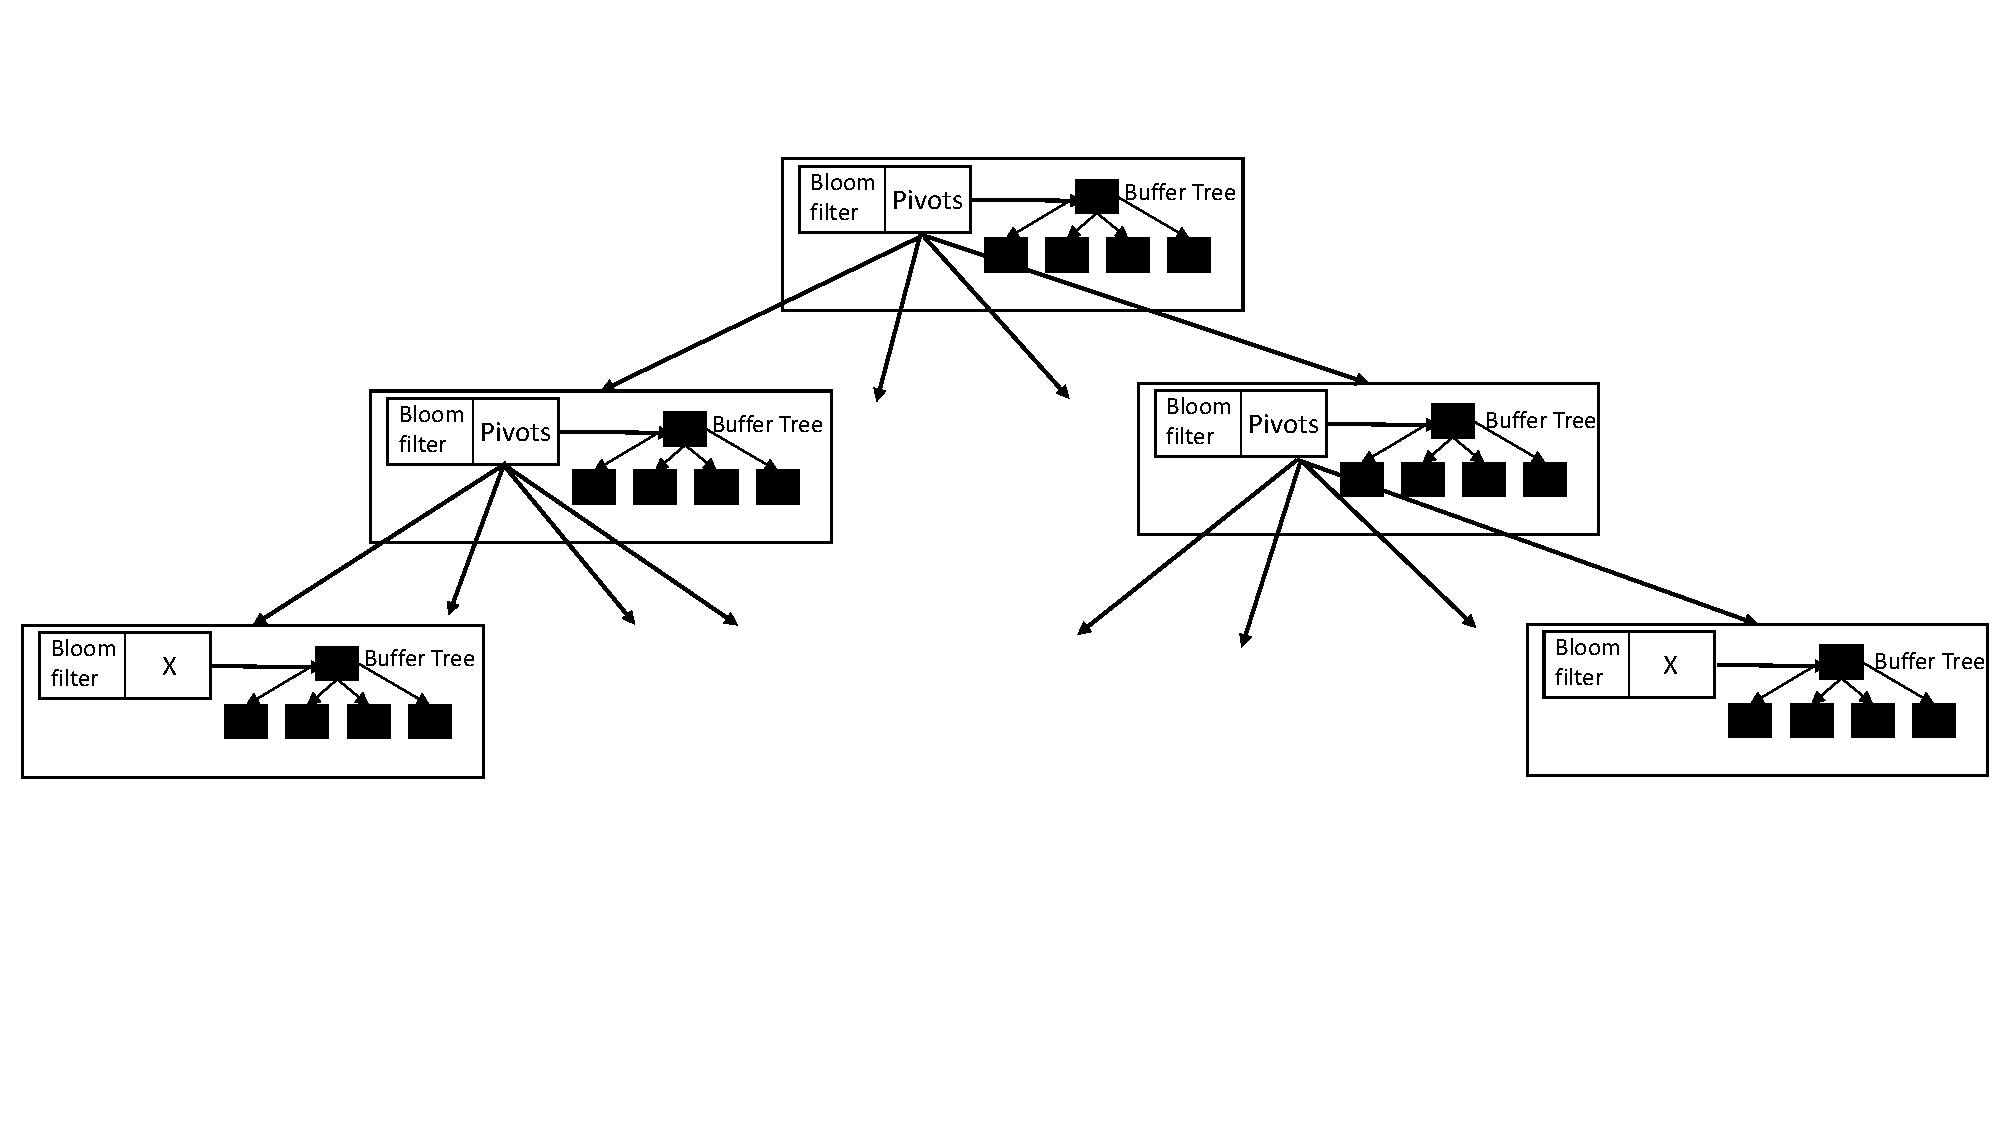
\includegraphics[scale=0.25]{wobtree.pdf}
%     \caption{The ``tree-of-trees'' \wobtreeone design.  Each \bet node
%       (indicated by white squares) stores its message buffer using a
%       B-tree (indicated by black squares).  The out square around each
%       \bet node and its buffer is purely illustrative---since this
%       data structure is designed for SSDs, there is no need to
%       maintain physical locality between a \bet node and the nodes of
%       its message buffer or between B-tree nodes belonging to the same
%       message buffer.}\label{fig:wobtree}
%   \end{center}
% \end{figure}

% The potential downside of using a B-tree is that, since the nodes of
% the B-tree might not be contiguous on disk, scanning the contents of a
% \bet node's buffer might require many disk I/Os.  However, the
% \wobtreeone is designed for SSDs, where locality is not so important
% as concurrency.  Thus, on SSDs, we can perform buffer scans at disk
% bandwidth, even if the B-tree nodes are not contiguous, by issueing
% multiple I/Os concurrently, so that the SSD always has a large number
% of I/O requests to serve concurrently (i.e. so that we maintain a high
% queue depth).

\section{High-Level Design of \datastructs}\label{sec:design}

We now describe the design features of \datastructs that give them 
low write amplification, low pass complexity, and high
concurrency, without sacrificing lookup performance.
%\subsection{Overall design}

\begin{figure}[t]
  \begin{center}
    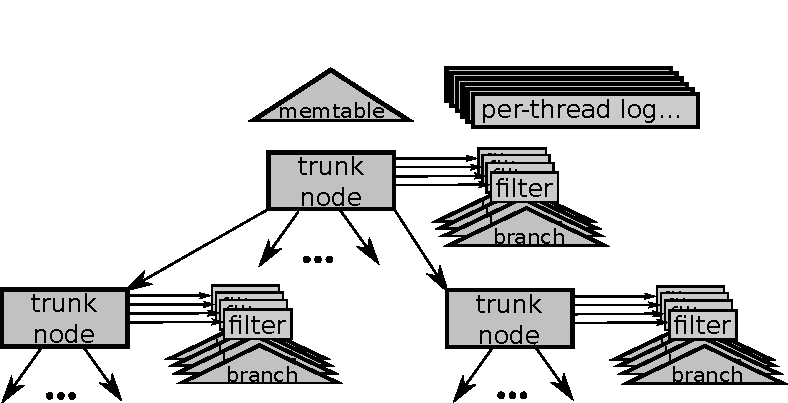
\includegraphics[width=3.25in]{figures/stbetree-diagram.pdf}
    \caption{Overall design of \datastructs and \sysname.  Trunk
      nodes contain pivots and child pointers and pointers to a
      collection of branches and their associated filters.  Each branch
      is a B-tree.  \sysname also keeps a queue of memtables to
      enable pipelining of memtable
      compactions.}
    \label{fig:stbetree}
  \end{center}
\end{figure}

At a high level, a \datastruct is a \bet, as shown in
\Cref{fig:stbetree}, albeit with several modifications to reduce I/O
amplification and exploit the I/O parallelism of NVMe devices.

On a spinning disk, data locality is paramount.  Thus, \bets designed
for spinning disks typically store each node, including pivots, child
pointers, and buffer contents, contiguously on disk.  Furthermore,
nodes are large---typically over a megabyte in size---in order to
amortize the cost of the seek required to access the node.  The
downside of large nodes is that they make point queries expensive.
Even if a point query has to load only a single leaf into cache, it
still has to transfer a megabyte or more of data.  Thus some \bets
divide their nodes into a header and physically contiguous
partitions.  The header contains pivots, child pointers, and an
index on the partitions, so that queries need only load the relevant
partition in a node.  Headers and partitions are typically 32-64KBs,
which is small enough to ensure that, on a hard drive, point query performance is seek
bound rather than bandwidth bound.

On NVMe, however, even transferring 32KB per query is too much.  For
example, on an Optane NVMe device, locality offers essentially no gain
in throughput, i.e. the device can deliver its full bandwidth via a
random I/O workload as long as the device queues are kept sufficiently
full.  Thus transferring 32KB per query would directly reduce maximum
query throughput to 1/8th of the device's random I/O throughput.

Consequently, our \datastruct strives not for locality, but rather for
low I/O amplification and high I/O parallelism.  Our \datastruct is a
tree of trees. The \defn{trunk tree} (or simply trunk) is analogous to
the headers of a traditional \bet, i.e. trunk nodes contain pivots,
child pointers, and pointers and metadata for the node's branches.
Trunk nodes are kept small---4KB in our implementation---so that they
do not waste cache space. In all practical use cases, trunk nodes
comprise less than $0.1\%$ of the total data and so are essentially
always cached.

Each \defn{branch} is a static B-tree, also with 4KB nodes in our
current implementation. Since each branch is constructed once and
never modified, the B-tree nodes are always fully packed, which
improves cache efficiency for point queries and reduces I/O
amplification during compactions and range queries.  Note that the
B-tree nodes of a branch are not necessarily stored contiguously on
disk, since locality is less important for utilizing the bandwidth of
NVMe devices. Range queries and compaction use the pointers in branch
nodes to prefetch leaves
in advance, enabling our \datastruct to take advantage of the I/O
parallelism of NVMe devices.

Each branch also has an associated \defn{quotient filter}. Quotient filters
serve the same role as Bloom filters in many LSM implementations.  However,
we choose quotient filters because they have substantially greater insert and
query performance than Bloom
filters~\cite{DBLP:journals/pvldb/BenderFJKKMMSSZ12}, reducing the CPU costs of
both queries and compactions, while using roughly the same or slightly less
space than Bloom filters for the false-positive rate used in \sysname (1/256).
Quotient filters are also efficient if they get paged out to disk, since each
lookup accesses only one page.

\sysname uses \defn{memtables} to collect new insertions.
Our memtable is a dynamic B-tree.  In fact, it is the same structure
as the B-trees used to store branches except that, since it is
dynamic, the nodes are not always fully packed.  When a memtable
fills, it is locked for new insertions, then the quotient filter is
constructed and then the memtable is inserted as a branch into the
trunk root.  No serialization or other work needs to happen.  When
former memtables participate in compactions, the resulting B-tree is
packed.

\sysname uses write-ahead logical logging for crash recovery.
\sysname uses per-thread logs to support highly concurrent updates.
Inter-log ordering is maintained by cross-referencing log entries with
timestamps on the leaves of the memtable (see \Cref{sec:recovery} for
details).

Note that all of the above data structures---memtables, trunk nodes,
branch nodes, filters and logs---are pageable.  \sysname has a unified
CLOCK cache for all these structures.

\section{Size-Tiering with Workload-Driven Compaction}\label{sec:flush-compact}

One of the goals of \sysname is to get both the benefits of size
tiering and the benefits of \bet's workload-driven compaction and
flushing.  Size-tiering reduces write amplification of all
workloads. Workload-driven compaction and flushing further reduces
write amplification when the workload is not uniformly random.
%% The challenge is that workload-driven flushing flushes from a parent
%% to only one child---the child with the most pending messages in the
%% parent.  How can we do this efficiently when the messages for the
%% child may be spread across multiple branches of the parent?
%% We describe below how \sysname solves this problem.
Our flushing and compaction algorithm is designed to preserve
worst-case performance guarantees of size-tiered LSM trees while
exceeding their performance on non-random workloads.  

The challenge is that a flushing and compaction algorithm must balance
two competing objectives.  First, we want to move data from one level
of the tree to the next in large batches.  This is the key reason
that LSMs and \bets are so much faster than B-trees for insertions.
On the other hand, we want to limit the number of locations that must
be searched during a query.  This means we cannot accumulate data
indefinitely before merging it into lower levels of the tree.

We begin by explaining the structure of \datastruct nodes.  This
structure will enable us to cleanly accomplish the above goals while
also enabling us to skip some compactions when the workload allows
it.

\textbf{Node structure.}  Each trunk node has a list of branches,
sorted from oldest to newest.  The trunk node also stores, for each
child, the index of the next branch to be flushed to that child.
Branches are flushed to a child in chronological order, so all older
branches have already been flushed to that child, and all newer
branches are yet to be flushed to that child.  We say that a branch is
\defn{live} for a child if it hasn't been flushed to that child.  We
say that a message in a branch is \defn{live} if the message's branch
is live for the message's target child.  Finally, each trunk node
stores, for each child, a rough estimate of the number of live
messages for that child across all the parent's branches.  This
estimate is made by scanning the top-level nodes of the branches and
estimating the amount of data in each subtree that falls entirely
within the pivots for a child.  Since branches are packed, these
estimates are quite accurate (typically to within less than 1\%).

Trunk nodes have a fixed number of branches that they can hold.  In
the current \sysname implementation, each trunk node can hold up to 84
branches.  However, trunk nodes begin flushing when they have $3F$
live branches, which is typically far less than 84 (e.g. $F$ is in the
range of 8 to 16).  This extra capacity is used to enable nodes to
absorb new incoming branches while compacting old branches.

Branches may be referenced by more than one trunk node.  Each trunk
node knows the range of keys that it covers so, for example, when a
parent and child both refer to the same branch, the parent might refer
to all the messages in the branch, while the child refers to only the
subset of messages in the branch for keys covered by the child.
Branches are immutable and refcounted, so sharing branches is safe.

This node structure and branch sharing means that we can ``flush'' a
live branch from a node to one of its children by simply adding a
pointer to the branch to the child. We can then mark the branch as
dead for that child in the parent.  If the branch becomes completely
dead in the parent (i.e. dead for all of its children), then the
parent can delete its references to the branch, decrementing the
branch's refcount.  Thus flushes are extremely cheap---just a few
pointer and refcount updates.

\textbf{Flush then Compact.}  \sysname avoids some intermediate
compactions by using a ``flush-then-compact'' approach.  Each flush
may trigger some compactions and some further, recursive flushes (see
below for a description of \sysname's flushing policy).  The idea of
flush-then-compact is to perform all the recursive flushes first.
Only once all the branches have been moved as far down the trunk as
possible do we begin performing compactions.  This will enable some
branches to skip intermediate compactions within the tree.

Once all the flushes from a node have completed, \sysname initiates
background compactions on all the nodes that recieved new branches.
Each background compaction compacts only the new branches in that node.
Thus no message gets compacted twice without being flushed from one
trunk node to another.

Compaction does not interfere with other concurrent tasks.  The trunk
node is not locked during the compaction---other threads may perform
queries or flush more branches to or from the trunk node.  During this
time, the compaction thread constructs a new branch that is the
compaction of all its input branches.  When the compaction thread
finishes, it briefly locks the trunk node to replace the old branch
pointers with a pointer to the new, compacted branch.

This mechanism also reduces contention at the root, since no
compactions are ever performed in the root.  Rather, whenever the root
fills, branches are moved to some of its children and compactions are
performed there, immediately making room for new items in the root.

Note that compactions skip over portions of the branches that are not
relevant to the compaction.  For example, when we flush branches from
the root to one of its children, the branches may contain keys outside
the range covered by that child.  When these branches get
compacted in the child, tthe compaction process won't
even look at those keys.  We can do this efficiently because branches
are B-trees that support iterators starting anywhere in the branch.

\textbf{Flushing policy.} 
The memtable has a maximum size of $m$ messages. 
Once it reaches size $m$, it is added as a
new branch to the root trunk node.

Flushes from a trunk node to one of its children are triggered by two
conditions: either the trunk node has more than $Fm$ live data, or one
of the trunk node's children has more than $3F$ live branches, where
$F$ is the fanout of the trunk.  These two conditions serve distinct
performance objectives.

The too-much-live-data trigger works with the compact-then-flush
algorithm to detect localized insertion workloads and move them
quickly down the tree without performing unnecessary intermediate
compactions.

For example, imagine a sequential insertion workload.  These inserts
first go to the memtable.  Once the memtable fills, it is added as a
branch to the root.  Once the root accumuates $F$ such branches, it
will go over the max-live-data threshold, causing a flush.  This flush
will move all the branches down the tree towards their target leaf.
This will immediately cause the child to exceed the max-live-data
threshold, so the branches will get flushed towards their target leaf
again.  This will repeat until the branches reach the leaf, at which
time \sysname will perform a compaction (and will probably split the
leaf).  The next batch of inserts will go to the new leaf created by
the split.  Thus each message will be involved in only a constant
number of compactions, giving $O(1)$ a write- and pass-complexity.

This method automatically adapts to varying degrees of
locality.  For example, if the workload is half inserts to a single
leaf, then every other time the root fills, we will perform a flush
from the root to the target leaf.  Or, if the workload consists of
random inserts of keys that all fall within a subtree $T$ of height,
say, $h/2$, then every time the root fills, \sysname will flush all
the branches to the root of the subtree without performing
intermediate compactions, skipping half the compactions that would
occur in a size-tiered LSM tree.

This policy does not weaken the worst-case insertion performance
guarantees of a size-tiered LSM: each message undergoes at most one
compaction per level of the tree, and the height of the tree is still
$\log_F N/m$.

The second flushing trigger is designed to bound the number of filters and
branches that must be examined during a query.  Whenever there are more than
$3hF$ branches on a search path (where $h$ is the height of the trunk), at
least one of the trunk nodes will violate the max-live-branches condition.
This will trigger a flush and compaction, which will reduce the number of
branches checked by queries along that path.

\section{Preemptive Splitting for \datastructs}
\label{sec:splitting}

Splits and merges pose problems for hand-over-hand locking in B-trees
(and \bets).  Hand-over-hand locking proceeds from root to leaf, but
splits and merges proceed from the leaves up.

An approach to solving this issue in B-trees is to use preemptive
splitting and merging~\cite{Rodeh08}.  During a B-tree insert, if a
child already has the maximum number of children, then it is split
while the insertion thread still holds a lock on its parent.  Then the
insertion can release the parent's lock and proceed down the tree,
assured that the child will not need to split again as part of this
insertion.  Analogously, deletions merge a child with one of its
neighbors if the child has the minimum number of children.  This works
because insertion and deletions can increase or decrease
the number of children of a node by at most 1.

This approach does not work in \bets, because a flush to a leaf could
cause that leaf to split multiple times.  In \datastruct with
flush-then-compact, we can move all pending messages along a
root-to-leaf path to the leaf before performing any compaction,
splits, or merges.  The total number of messages moved to the leaf is
bounded by $O(B\log_F N)$, i.e. the height of the tree times the
maximum amount of data that can be stored in branches at each trunk
node.  The leaf can therefore split into as many as $O(\log_F
N)$ new leaves of size $B$.  Similarly, a collection of flushes full
of delete messages to several leaves of a single parent can reduce the
parent's number of children by $O(\log_F N)$.

In practice, the height of the tree is less than 10 for typical
fanouts $F\approx 8$ and dataset size $N\leq 2^{80}$ key-value
pairs.

We extend preemptive splitting and merging to \datastructs as follows.
We reserve space in each node to accommodate up to $F + H$
children, where $H$ is an upper bound on the tree height, e.g. $H=10$.
We then apply preemptive splitting, except we preemptively split a
node during a flush if its fanout is above $F$.  For merges, we
take a similar approach.  If, during a flush, we encounter a node with
less than $F/2$ children, then we merge or rebalance it with one
of its siblings.

Thus all operations on the \datastruct---flushes, splits, and
merges---proceed from root to leaf and can therefore use
hand-over-hand locking.

The mechanisms for flush-then-compact make it easy to handle branches
during splits.  Recall that each branch can be marked dead or alive
for each child, and branches are refcounted and hence can be shared by
multiple trunk nodes. Thus we can split a trunk node by simply giving
its new sibling references to all the same branches as the node had
before the split.  In the new node, we copy the liveness information
for each branch along with the children that are moved to the new
sibling.

%% Therefore, preemptive
%% splitting is not enough to keep the number of pivots in the parent
%% below the maximum.  Restricting the flush rate to prevent this would
%% reduce update performance.

%% We solve this problem in \sysname's \bet by using \defn{postemptive} splitting.
%% Like preemptive splitting, this technique splits nodes as operations progress
%% down the tree with hand-over-hand locking. However, postemptive splitting only
%% splits nodes with \textit{more} pivots than the allowed maximum and is
%% permitted to temporarily exceed the maximum number of pivots in trunk index
%% nodes. Because fanout in a \bet is low, usually less than 20, there is more
%% than enough physical room in the node and then the split can be performed by
%% the next operation that touches the node.

\section{From \datastructs to \sysname}\label{sec:details} 
In this section, we discuss the details of \sysname's implementation. \sysname
targets NVMe SSDs, and on NVMe SSDs, CPU is the primary bottleneck to
write performance, and concurrency is the primary bottleneck to read
performance. As a result, what would be minor design decisions for a key-value
store which targets a slower storage medium become performance critical when
targeting NVMe storage.

\subsection{User-level Cache and Distributed Locks}\label{sec:cache}

\sysname{} has a single user-level cache which keeps recently accessed pages in
memory. Almost all the memory that \sysname uses comes from this cache, so
pages from all parts of the data structure---trunk node pages, branch pages,
filter pages and memtable pages---are all stored there. Only cache and
file-system metadata, as well as small allocations used to enqueue compaction
tasks are allocated from system memory.

This design allows nearly all the free memory to be used for whichever
operations are being performed, so that parts of the data structure which are
not in use can be paged out.

The cache at a high level is a clock cache, but with several features designed
to improve concurrency.

Each thread has a thread-local hand of the clock, which covers 64 pages. The
thread draws free pages from the hand, and if it has exhausted them, it
acquires a new hand from a global variable using a compare-and-swap. It then
writes out dirty pages from the hand which is a quarter turn ahead, and
evicts any evictable pages in its new hand. Thus threads clean and evict pages
from distinct cache lines within the cache metadata, avoiding contention and
cache-line ping-ponging.

\sysname uses distributed reader-writer locks~\cite{DBLP:conf/ipps/HsiehW92} to
avoid cache-line thrashing between readers.  Briefly, a distributed
reader-writer lock consists of a per-thread reader counter and a shared write
bit.  Each reader counter is on a separate cache line to avoid cache-line
ping-ponging when readers acquire the lock.  Writers set the write bit (using
compare and swap) and then wait for all the read counters to become zero.
Readers acquire the lock by incrementing their read counter and then checking
that the writer bit is 0.  If it is not, they decrement their reader counter
and restart.

Distributed reader-writer locks allow readers to scale essentially
perfectly linearly, at the cost that acquiring a write lock is
expensive.  However, the design of \sysname makes writing rare enough
that this is a good trade-off.

We make distributed reader-writer locks space efficent by storing each
thread's reader counters in an array indexed by cache-entry index.
Each reader counter is one byte, so the total space used by locks
is $t\times c$ bytes, where $t$ is the number of threads and $c$ is the
number of cache entries.

\sysname supports three levels of lock: read locks, ``claims'', and
write locks.  A claim is a read lock that can be upgraded to a write
lock.  Only one thread can hold a claim at a time.  After obtaining a
read lock, a thread may try to obtain a claim by trying to set a
shared claim bit with a test-and-set. If this fails, they must drop
the read lock and start over.  Otherwise, they can upgrade their claim
to a write lock by setting a shared write bit and waiting for all the
read counters to go to zero.

\subsection{Branch Trees and Memtables}
\sysname uses the same B-tree implementation for both its branches and its
memtables, although there are some differences to optimize for their use cases.
By using the same data structure, memtables can be incorporated into the 
\datastruct directly as branch trees with no serialization. The only processing
needed is the construction of a quotient filter.

\paragraph{Branch trees.}
When a branch is created from a compaction, its key-value pairs are packed into
the leaves of the B-tree, and the leading edge of internal nodes are created to
index them. The nodes in each level are allocated in extents of 32 pages, and
the header of each node stores the address of the following node, but also of
the next extent. In this way, the nodes of each level form a singly linked list.

Iteration through a branch is performed by walking the linked list
formed by its leaves.  Whenever the iterator reaches the beginning of
a new extent, it issues an asynchronus prefetch request for the next
extent.
%The extent length is configurable to tune to the latency of
%the storage device.

\paragraph{Memtables.}
The basic design of the memtables mirrors that of the branch B-trees, but
includes some optimizations designed to increase their insertion performance
and concurrency.

As in the case of the static branch trees, the nodes on each level of the
memtable form a singly-linked list, and nodes are allocated in extents.
However, because nodes are created on
demand as nodes split, we do not try to guarantee that successive nodes
reside in the same extent.  Furthermore, since memtables are almost always
in RAM, we do not perform prefetching during memtable traversals.

%% and in particular not in key order, the prefetching design of the
%% branch trees does not carry over. Therefore the memtables do not support
%% prefetching. In practice they are rarely written to disk, and overhead of
%% reading them without prefetching is only about 2--3$\times$.  \alex{probably
%% include some sort of statistic here.}

The memtable uses hand-over-hand locking, together with preemptive
splitting. At each index node, first a read lock is obtained, which is
upgraded only if a split is required. If an index node is full, the
inserter tries to upgrade it to a claim; if this fails, that means
another thread is already splitting the node, and the inserter
attempts to continue down the tree.  If it cannot continue because of
held locks, or if it finds that the leaf is full, then it aborts and
tries again from the root.

To ensure locks are held briefly, especially on nodes near the top of
the tree, the tree uses a new technique called \defn{shadow
  splitting}. To split a node $c$, a claim is obtained on $c$ and the
parent $p$. We allocate a physical block number (PBN) $n$ for the new
sibling, $c'$.  However, in the cache, we initially point $n$ to $c$.
We also add a new pivot to the parent $p$, pointing to the new PBN
$n$.  At this point, we can release all locks on $p$.  We then
allocate space for $c'$ and fill in its contents.  We then update the
PBN $n$ to point to $c'$ in the cache, and then release all locks on
$c'$.  Finally we upgrade to a write lock on $c$, truncate its child
list (via a metadata operation) and then release all locks on $c$.

%\subsection{Memtables}
%
%\rob{Maybe this should be expanded to explain the design of your
%  B-tree in general, including prefetching.}
%
%\sysname uses dynamic B-trees for its memtables. These B-trees use the same
%structure as the branch B-trees, except that they do not fully pack nodes. When
%a memtable fills, its quotient filter is constructed and it is added to the
%trunk root via a pointer swing. Because it shares the same structure as the
%branch B-trees, it needs no serialization or further processing.
%
%These memtables are designed to be kept in memory, but under cache pressure, it
%is possible that some or all of their pages will be written out to disk. When
%they are read back, they do not support the prefetching that the normal branch
%B-trees use. When they are scanned (\textit{e.g.} for compactions or scans),
%they are roughly 3--4$\times$ slower.
%
%In practice, this drawback doesn't significantly affect performance, because
%memtables are usually relatively short-lived. Even though memtables are added
%to the trunk root, once they are flushed from there, they will be compacted as
%per the compact-after-flush policy. Once they are flushed to all pivots, they
%will have no more references and be destroyed. The secondary flushing trigger
%(see \cref{sec:flush-compact}) guarantees that only so much data can be added
%to the trunk root before the memtable is flushed to all pivots, ensuring that
%the memtable will not live for very long.

\subsection{Quotient filters}

Bloom filters~\cite{DBLP:journals/cacm/Bloom70} are the standard filter for
most LSMs~\cite{leveldb,facebook-rocksdb2018,DBLP:conf/sosp/RajuKCA17}.
However, the cost of Bloom filter insertions can dominate the cost of sorting
the data in a compaction. Therefore modern key-value stores often use more
efficient filters; for example, RocksDB uses blocked Bloom
filters~\cite{DBLP:journals/jea/PutzeSS09};

Similarly, \sysname uses quotient
filters~\cite{DBLP:conf/hotstorage/BenderFJKMMSSZ11,DBLP:journals/pvldb/BenderFJKKMMSSZ12,DBLP:conf/sigmod/PandeyBJP17}
instead of Bloom filters.  A full presentation of quotient filters is
out of scope for this paper, but we review their salient features for
\sysname.  See Pandey, et al.\ for a full presentation on quotient
filters~\cite{DBLP:conf/sigmod/PandeyBJP17}.  The key feature of
quotient filters is that, like blocked Bloom filters, each insert or
query accesses $O(1)$ cache lines (and hence $O(1)$ page accesses).
Quotient filters are roughly as space efficient as Bloom filters---for
the range of parameters used in \sysname, quotient filters use between
$0.8\times$ and $1.2\times$ the space of a blocked Bloom filter.  We view
the space as essentially a wash.  Quotient filter inserts and lookups
also require only one hash function computation.  In past work,
quotient filter insertions and queries were shown to be 2-4$\times$
faster than in a Bloom filter.



%% A full presentation of quotient filters is out of
%% scope for this paper, but we review their salient features for \sysname.  A
%% quotient filter for set $S$ stores, without error, $h(S)=\{h(x) \mid x\in S\}$,
%% where $h$ is a hash function.  Since the quotient filter stores $h(S)$ exactly,
%% all false positives are the result of collisions under $h$.  Thus each
%% insertion or lookup requires only one hash function computation.  Furthermore,
%% a quotient filter stores the elements of $h(S)$ in sorted order in a hash table
%% using a variant of linear probing.  Thus most inserts and lookups in a quotient
%% filter access only 1 or 2 adjacent cache lines.  As a result, insertions and
%% lookups in quotient filters are typically 2-4$\times$ faster than in a Bloom
%% filter.  Finally, quotient filters are space efficient, using slightly less
%% space than Bloom filters whenever the false positive rate $\epsilon$ is less
%% than $1/64$, which is typical.  For example, a quotient filter with
%% $\epsilon=0.1\%$ uses about 10\% less space than a Bloom
%% filter~\cite{DBLP:conf/sigmod/PandeyBJP17}.

\sysname further reduces the CPU costs of filter building during compaction by
using a bulk build algorithm.  During the merging phase of compaction or when
inserting into a memtable, \sysname builds an unsorted array of all the hashes
of all the tuples compacted or inserted. The array is then sorted (by hash
value) and the quotient filter is built.  Since the quotient filter also stores
the hashes in sorted order, this means that the process of inserting all the
hashes is a linear scan of the sorted array and of the quotient filter.  Hence
it has good locality and can benefit from cache prefetching.  

\subsection{Logging and Recovery}
\label{sec:recovery}

\sysname uses per-thread write-ahead logical logging for recovery.  By
using per-thread logs, we avoid contention on the head of a single,
shared log.

The challenge is to resolve the order of operations across logs after
a crash.  For this, we use a technique similar to ``cross-referenced
logs''~\cite{DBLP:conf/usenix/HuangPMS0B18}.  Our scheme works as
follows.  Each leaf of the memtable has a generation number.  Whenever
a thread inserts a new message into the memtable, it records and
increments the generation number of the memtable leaf for the inserted
key.  It then appends the inserted message to its per-thread log,
tagged with the leaf's generation number.  During recovery, the
generation numbers in the logs give a total order on the operations
performed on each leaf (and hence on all the keys for that leaf), so
that the recovery procedure can replay the operations on each key in
the proper order.  When a leaf of the memtable splits, the new leaf
gets the same generation number as the old leaf.

%% Checkpoints proceed as follows.  A checkpoint begins by incorporating
%% the current memtable into the \datastruct and copying the entire trunk
%% of the \datastruct, creating a new trunk that shares all its branches
%% with the running trunk.  Since branches are all immutable and
%% reference-counted, they can safely be shared between the live tree and
%% the tree that is in the process of being checkpointed.  The copy is
%% created in a breadth-first manner with hand-over-hand locking,
%% ensuring that the copy is a consistent view of the \datastruct's
%% logical state at the moment when the copy began.  Since each trunk
%% node covers, on average, hundreds of megabytes of messages, the number
%% of trunk nodes is extremely small---typically only a few thousand---so
%% the copy operation takes very little time.  The checkpointing process
%% also records the positions of the heads of all the per-thread logs.

%% Once \sysname has created a copy of the trunk, it makes a single pass
%% over the cache, writing out all dirty pages.  This ensures that all
%% pages referenced by the in-progress checkpoint tree are on disk.

%% Finally, \sysname has two superblocks, each of which points to the
%% root of a \datastruct and its associated logs.  The two superblocks
%% are timestamped and, on boot, \sysname chooses the more recent of the
%% two.  Thus, to complete a checkpoint, \sysname overwrites the older of
%% the two superblocks with a new block containing pointers to the new
%% trunk and to the heads of the logs that were recorded earlier.  After
%% writing out this new superblock, all log pages prior to the log heads
%% can be garbage collected.

\section{Evaluation}\label{sec:eval}

We evaluate the performance of \sysname{} on several microbenchmarks and on the
standard YCSB application benchmark\cite{DBLP:conf/cloud/CooperSTRS10}. We
compare this performance against that of two state-of-the-art key-value stores,
RocksDB and PebblesDB.  The following questions drive our evaluation:
%In our evaluation, we first wish to demonstrate \sysname's macro performance.
%Then, we would like to understand the performance impacts of several specific
%design decisions in \sysname, and to quantify both the advantages and drawbacks
%of these choices. Specifically we hope to answer the following questions:
\begin{itemize}
   \item Does \sysname achieve its primary goal of improved insertion
      performance?
   \item To what extent is this performance achieved through reduced write
      amplification as opposed to other factors?
   \item Does increasing insert performance come at a cost to [range] query
     performance?  In particular, do queries in \sysname require more I/O, due to
     size tiering, than in non-size-tiered systems?
   \item Are sequential (or otherwise local) insertions faster as predicted on
     \sysname? Do they have lower write amplification?
   \item Can \sysname utilize device bandwidth for large range queries?
   \item \sysname is designed to be highly concurrent; do point lookups scale
      with the number of threads?
\end{itemize}

\subsection{Setup and Workloads}\label{sec:setup}

All results are collected on a Dell PowerEdge R720 with a 32-core
2.00 GHz Intel Xeon CPU, 256 GiB RAM and a 960GiB Intel Optane 905p PCI Express
3.0 NVMe device. The block size used was 4096 bytes.

In general, we use workloads derived from YCSB traces with 24B keys. We
generally use 100B values, but also include a set of YCSB benchmarks for 1KiB
values.  We instrumented dry runs of YCSB in order to collect workload traces
for the load and $A-F$ YCSB workloads and replay them on each of the databases
evaluated.  In order to eliminate the overhead of reading from a trace file
during the experiment, the trace replayer \texttt{mmap}s the trace file before
starting the experiment.  We use the same traces for each system.

In general, we limit the available memory to 10\% of the dataset size or less.
In order to perform the benchmarks on reasonably sized datasets, we restrict
the available system memory with a type 1 Linux \texttt{cgroup}, sized to the
target memory size plus the size of the trace, which we pin so that it cannot
be swapped out. Unless otherwise noted, the target memory size is 4GiB.
PebblesDB has an apparent memory leak, which causes it to consume the available
memory, so we allow it to use the full system memory. On the YCSB load
benchmarks, this causes it to swap for a small portion at the end, but this was
less than 10\% of the  run time.

Unless otherwise noted, \sysname{} uses a max fanout of 8, a memtable size of
24MiB and a total cache size of 3.25GiB. The difference between this cache size
and the target memory size of 4GiB is to accommodate other in-memory data
structures maintained by \sysname.

Each system is run with the thread count which yields the highest throughput.
RocksDB is configured to use background threads equal to the number of cores
minus the number of foreground threads, with a minimum of 4. PebblesDB uses its
default number of background compaction threads. \sysname is configured without
background compaction threads.

\subsection{YCSB}\label{sec:ycsb}

We measure application performance using the Yahoo Cloud Services Benchmark
(YCSB). The core YCSB workloads consist of load phases and run phases.
The load phases create a dataset by inserting uniformly random
key-value pairs. 
The run phases emulate various workload mixes. Workload A is 
50\% updates, 50\% reads, workload B is 95\% reads, 5\%
updates), workload C is 100\% reads, workload D is read latest (95\%
reads, 5\% insertions), workload E is short range scans (95\% scans, 5\% insertions)
and workload F is read-modify-writes (50\% reads, 50\% RMWs).

The results with 100B values is shown in 
 \Cref{fig:ycsb-100B,fig:ycsb-amp-100B}, and we also use a version
with 24B keys and 1kib values \alex{need this figure}.  

On the load phase, \sysname is faster by almost an order of magnitude.  Because
of size-tiering and its compaction/flushing policy \sysname has about $1/2$ the
write amplification of the other systems. Note PebblesDB performs almost no
reads because it was given unlimited memory.  Surprisingly PebblesDB does not
show substantially lower write amplification than RocksDB.

On the run phases, which the exception of E, \sysname is 40--150\% faster than
RocksDB, the next fastest system. On E, \sysname is roughly half as fast as
RocksDB.

\begin{figure*}
      \centering
      \ref{ycsb-legend} \\
      \begin{subfigure}{0.52\linewidth}
         \begin{tikzpicture}
            \begin{axis}[
                  ybar=1pt,
                  bar width=5.5pt,
                  enlarge x limits=0.1,
                  width = \columnwidth,
                  height = 1.75in,
                  symbolic x coords = {Load, A, B, C, D, E, F},
                  xtick = data,
                  major x tick style = transparent,
                  ymin = 0,
                  ymax = 2750,
                  yticklabel style = {rotate=90},
                  ylabel near ticks,
                  /pgf/number format/1000 sep={},
                  nodes near coords,
                  every node near coord/.append style={rotate=90, anchor=west, font=\tiny},
                  ylabel={Operations/Second \\ (Thousands)},
                  xlabel={YCSB Workload (24B keys, 100B values)},
                  label style={font=\small, align=center},
                  legend columns=5,
                  %legend style={at={(0.98, 0.98)}, anchor=north east}
                  legend to name={ycsb-legend}
               ]
               \addplot[style={Plum,fill=Plum,mark=none} ]
               table [col sep=space] {data/ycsb-100b/splinterdb.csv};
               \addplot[style={RoyalBlue,fill=RoyalBlue,mark=none}]
               table [col sep=space] {data/ycsb-100b/rocksdb.csv};
               \addplot[style={ForestGreen,fill=ForestGreen,mark=none}]
               table [col sep=space] {data/ycsb-100b/pebblesdb.csv};
               \legend{\sysname, RocksDB, PebblesDB};
            \end{axis}
         \end{tikzpicture}
         \caption{Throughput on YCSB workloads with 24B keys and 100B values.
         Load is 673M operations, E is 20M operations and others are 160M
         operations. Higher is better.}\label{fig:ycsb-100B}
      \end{subfigure}
      \hspace{0.0\linewidth}
      \begin{subfigure}{0.40\linewidth}
         \centering
            \begin{tikzpicture}
               \begin{axis}[
                     ybar=1pt,
                     bar width=5.5pt,
                     enlarge x limits=0.1,
                     width = \columnwidth,
                     height = 1.75in,
                     symbolic x coords = {Load, A, B, C, D, E, F},
                     xtick = data,
                     major x tick style = transparent,
                     ymin = 0,
                     ymax = 900,
                     yticklabel style = {rotate=90},
                     ylabel near ticks,
                     /pgf/number format/1000 sep={},
                     nodes near coords,
                     every node near coord/.append style={rotate=90, anchor=west, font=\tiny},
                     ylabel={Operations/Second \\ (Thousands)},
                     xlabel={YCSB Workload (24B keys, 1KiB values)},
                     label style={font=\small, align=center},
                     legend columns=1,
                     legend style={at={(0.98, 0.98)}, anchor=north east}
                     %legend to name={ycsb-legend}
                  ]
                  \addplot[style={Plum,fill=Plum,mark=none} ]
                  table [col sep=space] {data/ycsb-1kib/splinterdb.csv};
                  \addplot[style={RoyalBlue,fill=RoyalBlue,mark=none}]
                  table [col sep=space] {data/ycsb-1kib/rocksdb.csv};
                  %\addplot[style={ForestGreen,fill=ForestGreen,mark=none}]
                  %table [col sep=space] {data/ycsb-1kib/pebblesdb.csv};
                  %\legend{\sysname, RocksDB};%, PebblesDB};
            \end{axis}
         \end{tikzpicture}
         \caption{Throughput on YCSB workload with 24B keys and 1KiB values.
         Load is 84M operations, E is 1.3M operations and others are 10M
         operations. Higher is better.}\label{fig:ycsb-1kib}
      \end{subfigure}
      \caption{YCSB throughput and I/O benchmark results.}
\end{figure*}

\begin{figure}
   \begin{tikzpicture}
      \begin{axis}[
            ybar=1pt,
            bar width=10pt,
            enlarge x limits=0.3,
            width = \columnwidth,
            height = 1.35in,
            symbolic x coords = {load-write, load-total, c-read},
            xticklabel style = {align=center},
            xticklabels = {Load:\\Write Amp, Load:\\Total I/O Amp, Run C:\\Read Amp},
            xtick = data,
            xticklabel style = {font=\small},
            major x tick style = transparent,
            ymin = 0,
            ymax = 37,
            ylabel={I/O Amplification},
            ylabel near ticks,
            xlabel={YCSB IO Amplification (24B keys, 100B values)},
            label style = {font=\small},
            nodes near coords,
            every node near coord/.append style={font=\scriptsize},
            nodes near coords style={/pgf/number format/.cd, fixed zerofill, precision=1},
            %legend columns=1,
            %legend style={font=\scriptsize, at={(0.02, 0.98)}, anchor=north west},
         ]
         \addplot[style={Plum,fill=Plum,mark=none}]
         table [col sep=space] {data/ycsb-amp-100b/splinterdb.csv};
         \addplot[style={RoyalBlue,fill=RoyalBlue,mark=none}]
         table [col sep=space] {data/ycsb-amp-100b/rocksdb.csv};
         \addplot[style={ForestGreen,fill=ForestGreen,mark=none}]
         table [col sep=space] {data/ycsb-amp-100b/pebblesdb.csv};
         %\legend{\sysname, \sysname (12 threads), RocksDB, PebblesDB};
      \end{axis}
   \end{tikzpicture}
   \caption{IO amplification on YCSB load and Run C workloads, as
   measured with iostat. Lower is better.}\label{fig:ycsb-amp-100B}
\end{figure}

\subsection{KVell}\label{sec:kvell}

KVell~\cite{DBLP:conf/sosp/LepersBGZ19} is a key-value store also designed to
utilize full NVMe bandwidth.  It has an in-memory B-tree index that maps all
keys to disk page offsets.  It does well on large (4KiB) key-value pairs, but
on small key-value pairs, the overhead of the in-memory index becomes a
significant fraction of the dataset size.  In particular, it was impossible to
run KVell in a memory \texttt{cgroup} of 4GiB.  Figure~\ref{fig:kvell} shows
KVell's performance on the YCSB workload with 100B values, for different memory
sizes. At 22GiB, which is around the size of the in-memory index, KVell's
performance starts to drop. At 20GiB, KVell becomes unusable. Therefore in
realistic memory settings, KVell is not a viable option for the small key-value
sizes that \sysname targets.

\begin{figure}
   \begin{tikzpicture}
      \begin{axis}[
            ybar=1pt,
            bar width=3.5pt,
            enlarge x limits=0.1,
            width = \columnwidth,
            height = 1.85in,
            symbolic x coords = {Load, A, B, C, D, E, F},
            xtick = data,
            major x tick style = transparent,
            ymin = 0,
            ymax = 3700,
            yticklabel style = {rotate=90},
            ylabel near ticks,
            /pgf/number format/1000 sep={},
            nodes near coords,
            every node near coord/.append style={/pgf/number format/fixed, rotate=90, anchor=west, font=\tiny},
            ylabel={Operations/Second \\ (Thousands)},
            xlabel={YCSB Workload (24B keys, 100B values)},
            label style = {font=\small, align=center},
            legend columns=2,
            legend style={at={(0.98, 0.98)}, anchor=north east, font=\scriptsize}
            %legend to name={ycsb-legend}
         ]
         \addplot[style={Red,fill=Red!25!white,mark=none} ]
         table [col sep=space] {data/ycsb-100b/kvell20.csv};
         \addplot[style={Red,fill=Red!50!white,mark=none} ]
         table [col sep=space] {data/ycsb-100b/kvell22.csv};
         \addplot[style={Red,fill=Red,mark=none} ]
         table [col sep=space] {data/ycsb-100b/kvell24.csv};
         \addplot[style={Red,fill=Red!50!black,mark=none} ]
         table [col sep=space] {data/ycsb-100b/kvell26.csv};
         \addplot[style={Red,fill=Red!25!black,mark=none} ]
         table [col sep=space] {data/ycsb-100b/kvell28.csv};
         \legend{20GiB, 22GiB, 24GiB, 26GiB, 28GiB};
      \end{axis}
   \end{tikzpicture}
   \caption{Throughput of Kvell on YCSB workloads with varying amounts of
   available RAM. Load consists of 673M operations, E consists of 20M
   operations and all other workloads consist of 160M operations. Higher is
   better.}\label{fig:kvell}
\end{figure}

\subsection{Sequential Insertion Performance}\label{sec:seq}

Because \sysname{} is based on an \datastruct{} and makes use of a
flush-then-compact policy, we predict that its performance will
improve substantially on insertion workloads with a high degree of
locality (see \cref{sec:flush-compact}). We test this hypothesis by
performing 20GiB of single-threaded insertions from a trace composed of
interleaved sequential and random keys in different proportions. For
comparison, we perform the same workload on RocksDB.

As shown in \cref{fig:sequential}, \sysname's performance improves smoothly
from 349K insertions per second for a purely random workload to 614K insertions
per second for a purely sequential workload, which is 76\% faster. This
improvement is partially obscured by the log, which adds a constant additive IO
overhead. If we disable the log, \sysname improves from 430K insertions per
second on a purely random workload to 866K operations per second on a purely
sequential workload, 100\% faster. Note that we would expect the intermediate
throughputs in the best case to be the [weighted] harmonic mean of the pure
cases, because they are rates. At 50\% random, 50\% sequential for \sysname
with no log this is 575K insertions/second, so its actual performance of 521K
insertions/second captures a substantial amount of the potential improvement.

RocksDB also improves as the workload becomes more sequential, but this effect
is much smaller, a 35\% speedup. Furthermore, RocksDB shows less than 20\%
speedup until the workloads becomes 99\% sequential.

\Cref{fig:sequential-amp} shows that as predicted, \sysname incurs less IO
amplification on more sequential workloads. With the log disabled, its write
amp approaches 1 as the workload approaches purely sequential.  In contrast,
while RocksDB also has less IO amplification on more sequential workloads, it
still incurs write amplification of 4.1 even when 99\% of the keys are
sequential. It is only when the workload becomes 100\% sequential that the
write amplification becomes close to 1 (because of caching it even falls below
1).

\begin{figure*}
  \centering
  \ref{seq-legend} \\
  \begin{subfigure}{0.45\linewidth}
   \begin{tikzpicture}
      \begin{axis} [
            width = \columnwidth,
            height = 1.75in,
            xtick = data,
            ytick distance = 500,
            minor y tick num = 4,
            enlarge x limits = 0.05,
            symbolic x coords = {0, 50, 90, 99, 100},
            %major x tick style = transparent,
            ymin = 0,
            ymax = 999,
            ylabel={Operations/Second \\ (Thousands)},
            yticklabel style = {rotate=90},
            ylabel near ticks,
            label style = {font=\small, align=center},
            xmin = 0,
            xmax = 100,
            nodes near coords,
            xlabel={Percentage Sequential Insertions},
            %legend cell align={left},
            legend to name=seq-legend,
            legend columns=3,
            %legend style={at={(0.02, 0.98)}, anchor=north west}
         ]
      \addplot [
         style={Plum},
         line width=1.5pt,
         mark=*,
         visualization depends on=\thisrow{Alignment} \as \alignment,
         %visualization depends on=\thisrow{YShift} \as \yshift,
         every node near coord/.append style={font=\scriptsize, anchor=north}
      ]
         table [
            col sep=space,
         ] {data/sequential/splinterdb.csv};
      \addplot [
         style={VioletRed},
         line width=1.5pt,
         mark=*,
         %visualization depends on=\thisrow{Alignment} \as \alignment,
         %visualization depends on=\thisrow{YShift} \as \yshift,
         every node near coord/.append style={font=\scriptsize, anchor = south},
      ]
         table [
            col sep=space,
         ] {data/sequential/splinterdb-no-log.csv};
      \addplot [
         style={RoyalBlue},
         line width=1.5pt,
         mark=square*,
         visualization depends on=\thisrow{Alignment} \as \alignment,
         %visualization depends on=\thisrow{YShift} \as \yshift,
         every node near coord/.append style={font=\scriptsize, anchor=south}
      ]
         table [
            col sep=space,
         ] {data/sequential/rocksdb.csv};
         \legend{\sysname, \sysname (no log), RocksDB};
      \end{axis}
   \end{tikzpicture}
   \caption{Single-threaded insertion throughput by locality. X-axis indicates
   the percentage of sequential keys.  X-axis not to scale. Higher is
   better.}\label{fig:sequential}
\end{subfigure}
\hspace{0.075\linewidth}
\begin{subfigure}{0.45\linewidth}
   \begin{tikzpicture}
      \begin{axis} [
            width = \columnwidth,
            height = 1.75in,
            xtick = data,
            minor y tick num = 4,
            symbolic x coords = {0, 50, 90, 99, 100},
            enlarge x limits = 0.05,
            %major x tick style = transparent,
            ymin = 0,
            ymax = 14.9,
            ylabel={I/O Amplification},
            yticklabel style = {rotate=90},
            ylabel near ticks,
            label style = {font=\small},
            xmin = 0,
            xmax = 100,
            xlabel={Percentage Sequential Insertions},
            %legend cell align={left},
            %legend style={at={(0.98, 0.98)}, anchor=north east},
            %legend columns = 1
         ]
      \addplot [
         style={Plum},
         line width=1pt,
         mark=*,
         nodes near coords,
         %visualization depends on=\thisrow{WriteAlignment} \as \alignment,
         %visualization depends on=\thisrow{WriteOpacity} \as \opacity,
         every node near coord/.append style={font=\scriptsize, anchor=south, rotate = 0},
      ]
         table [
            col sep=space,
            y=Write,
         ] {data/sequential-amp/splinterdb.csv};
      \addplot [
         style={Plum},
         line width=1pt,
         mark=o,
         mark options={solid},
         %dashed,
         %nodes near coords,
         %visualization depends on=\thisrow{TotalAlignment} \as \alignment,
         %every node near coord/.append style={font=\scriptsize, anchor=\alignment},
         forget plot
      ]
         table [
            col sep=space,
            y=Total
         ] {data/sequential-amp/splinterdb.csv};
      \addplot [
         style={VioletRed},
         line width=1pt,
         mark=*,
         nodes near coords,
         %visualization depends on=\thisrow{WriteAlignment} \as \alignment,
         %visualization depends on=\thisrow{WriteOpacity} \as \opacity,
         every node near coord/.append style={font=\scriptsize, anchor=north, rotate = 0},
      ]
         table [
            col sep=space,
            y=Write,
         ] {data/sequential-amp/splinterdb-no-log.csv};
      \addplot [
         style={VioletRed},
         line width=1pt,
         mark=o,
         mark options={solid},
         dashed,
         %nodes near coords,
         %visualization depends on=\thisrow{TotalAlignment} \as \alignment,
         %every node near coord/.append style={font=\scriptsize, anchor=\alignment},
         forget plot
      ]
         table [
            col sep=space,
            y=Total
         ] {data/sequential-amp/splinterdb-no-log.csv};
      \addplot [
         style={RoyalBlue},
         line width=1pt,
         mark=square*,
         nodes near coords,
         %visualization depends on=\thisrow{WriteAlignment} \as \alignment,
         %visualization depends on=\thisrow{WriteOpacity} \as \opacity,
         every node near coord/.append style={font=\scriptsize, anchor=south, rotate = 0},
      ]
         table [
            col sep=space,
            y=Write
         ] {data/sequential-amp/rocksdb.csv};
      \addplot [
         style={RoyalBlue},
         line width=1pt,
         mark=square,
         mark options={solid},
         dashed,
         %nodes near coords,
         %visualization depends on=\thisrow{TotalAlignment} \as \alignment,
         %every node near coord/.append style={font=\scriptsize, anchor=\alignment},
         forget plot
      ]
         table [
            col sep=space,
            y=Total
         ] {data/sequential-amp/rocksdb.csv};
         %\legend{\sysname, \sysname (no log), RocksDB};
      \end{axis}
   \end{tikzpicture}
   \caption{I/O amplification of mixed sequential/random insertion
     workloads. Shown are write amplification (solid) and
     total IO amplification (dashed) as measured with
     \texttt{iostat}. X-axis not to scale. Lower is
     better.}\label{fig:sequential-amp}
\end{subfigure}
\caption{Insertion throughput and I/O amplification as a function of workload locality.}
\end{figure*}


\subsection{Concurrency Scaling}\label{sec:scaling}

\Sysname is designed to scale with the number of available cores up to the
performance limits of the storage device. This is especially true for reads,
where the use of distributed reader-writer locks and a highly concurrent cache
design, together with a careful avoidance of dirtying cache lines, can avoid
almost all contention between threads.

\paragraph{Read Concurrency}
We test the read concurrency scaling of \sysname{} by running YCSB
workload C with 160M key-value pairs, where (as in \cref{fig:ycsb-100B} each
instance of the test divides the keys into $N$ evenly divided batches, which
are then performed in parallel by $N$ threads. The results are in
\cref{fig:read-concurrency}.

The results show nearly linear scaling---throughput with 24 threads is
18.5$\times$ the single-threaded throughput. Between roughly 24 and 32 threads,
the scaling flattens out, but at that point the measured throughput is
2.07--2.24 GiB/sec, which is 88--95\% of the device's advertised random read
capability.

While RocksDB also scales well, its throughput with 24 threads is 17.4$\times$
its single-threaded throughput, and with 32 threads it uses 91\% of the
device's advertized random read capability. Therefore, even though \sysname can
perform more operations per second, RocksDB is still making nearly full use of
the device for reads. We conclude here that SplinterDB is making better use of
the available memory for caching, since it has noticeably lower read
amplification.

\alex{Say something about Pebbles?}

\paragraph{Insertion Concurrency}
We test the insertion concurrency scaling of \sysname by running the YCSB load
workload with 673M key-value pairs divided into $N$ batches, each of which
is inserted in parallel by a different thread. \cref{fig:write-concurrency}
shows selected $N$ for each system, including its peak throughput.

The results show that \sysname scales almost linearly up to 10 threads. With
10+ threads, it performs 2.0-2.4M insertions per second with IO amplification
around 7.5, which implies that it uses 1.9-2.2GiB/sec of bandwidth, which is at
or near the device's sequential bandwidth of 2.2GiB/sec.

RocksDB's insertion performance also scales as the number of threads increase
up to 14 threads, by a factor of 2.7. At its peak, it uses 754GiB/sec of
bandwidth. PebblesDB scales slightly as well.  For both RocksDB and PebblesDB,
as many background threads as available are used for flushing and compaction
during this benchmark.

\begin{figure}
   \begin{tikzpicture}
      \begin{axis} [
            width = \columnwidth,
            height = 0.7\columnwidth,
            xtick distance = 4,
            major x tick style = transparent,
            ymin = 0,
            ymax = 950,
            yticklabel style = {rotate=90},
            ylabel={Operations/Second (Thousands)},
            xlabel={Number of Concurrent Threads},
            label style = {font=\small},
            xmin = 0,
            xmax = 32,
            legend style={at={(0.02, 0.98)}, anchor=north west, font=\small}
         ]
      %\draw[dotted, very thick] (axis cs: 0,669) -- (axis cs: 33,669)
      %   node[pos=.65, above] {relative device limit};
      \addplot [
         style={Plum},
         line width=1.5pt,
         mark=*,
         nodes near coords,
         visualization depends on=\thisrow{Alignment} \as \alignment,
         visualization depends on=\thisrow{YShift} \as \yshift,
         %visualization depends on=\thisrow{Opacity} \as \opacity,
         every node near coord/.append style={font=\scriptsize, anchor=west, rotate=90}
      ]
         table [
            col sep=space,
         ] {data/read-concurrency/splinterdb.csv};
      \addplot [
         style={RoyalBlue},
         line width=1.5pt,
         mark=square*,
         nodes near coords,
         visualization depends on=\thisrow{Alignment} \as \alignment,
         visualization depends on=\thisrow{YShift} \as \yshift,
         visualization depends on=\thisrow{Opacity} \as \opacity,
         every node near coord/.append style={font=\scriptsize, anchor=west, rotate = 330}
      ]
         table [
            col sep=space,
         ] {data/read-concurrency/rocksdb.csv};
      \addplot [
         style={ForestGreen},
         line width=1.5pt,
         mark=triangle*,
         nodes near coords,
         visualization depends on=\thisrow{Alignment} \as \alignment,
         visualization depends on=\thisrow{YShift} \as \yshift,
         visualization depends on=\thisrow{Opacity} \as \opacity,
         every node near coord/.append style={font=\scriptsize, anchor=north west, rotate = 330}
      ]
         table [
            col sep=space,
         ] {data/read-concurrency/pebblesdb.csv};
         \legend{\sysname, RocksDB, PebblesDB};
      \end{axis}
   \end{tikzpicture}
   \caption{Read throughput performance (YCSB workload C) by number of threads.
   Each instance performs 160M reads divided evenly between threads. Higher is
   better.}\label{fig:read-concurrency}
\end{figure}

\begin{figure}
   \begin{tikzpicture}
      \begin{axis} [
            width = \columnwidth,
            height = 0.6\columnwidth,
            xtick distance = 4,
            major x tick style = transparent,
            ymin = 0,
            ymax = 2499,
            yticklabel style = {rotate=90},
            ylabel={Operations/Second \\ (Thousands)},
            xlabel={Number of Concurrent Threads},
            label style = {font=\small, align=center},
            xmin = 0,
            xmax = 32,
            legend style={at={(0.95, 0.5)}, anchor=east, font=\small}
         ]
      %\draw[dotted, very thick] (axis cs: 0,669) -- (axis cs: 33,669)
      %   node[pos=.65, above] {relative device limit};
      \addplot [
         style={Plum},
         line width=1.5pt,
         mark=*,
         nodes near coords,
         visualization depends on=\thisrow{Alignment} \as \alignment,
         visualization depends on=\thisrow{YShift} \as \yshift,
         every node near coord/.append style={font=\scriptsize, anchor=west,yshift=-1,rotate=-45}
      ]
         table [
            col sep=space,
         ] {data/write-concurrency/splinterdb.csv};
      \addplot [
         style={RoyalBlue},
         line width=1.5pt,
         mark=square*,
         nodes near coords,
         visualization depends on=\thisrow{Alignment} \as \alignment,
         visualization depends on=\thisrow{YShift} \as \yshift,
         every node near coord/.append style={font=\scriptsize, anchor=west,rotate=90}
      ]
         table [
            col sep=space,
         ] {data/write-concurrency/rocksdb.csv};
         \legend{\sysname, RocksDB};
      \addplot [
         style={ForestGreen},
         line width=1.5pt,
         mark=triangle*,
         nodes near coords,
         visualization depends on=\thisrow{Alignment} \as \alignment,
         visualization depends on=\thisrow{YShift} \as \yshift,
         every node near coord/.append style={font=\scriptsize, anchor=south east,rotate=0}
      ]
         table [
            col sep=space,
         ] {data/write-concurrency/pebblesdb.csv};
         \legend{\sysname, RocksDB, PebblesDB};
      \end{axis}
   \end{tikzpicture}
   \caption{Write throughput performance (YCSB Load) by number of threads.
   Each instance performs 673M writes divided evenly between threads.  Higher
   is better.}\label{fig:write-concurrency}
\end{figure}

\subsection{Scan Performance}\label{sec:scan}

\begin{figure}
   \begin{tikzpicture}
      \begin{axis} [
            width = \columnwidth,
            height = 0.6\columnwidth,
            xmode = log,
            %xtick = data,
            major x tick style = transparent,
            /pgf/number format/1000 sep={},
            ylabel near ticks,
            label style = {font=\small, align=center},
            xmin = 1,
            xmax = 100000,
            enlarge x limits=0.1,
            ymin = 0,
            ymax = 2990,
            yticklabel style = {rotate=90},
            ylabel={Effective Throughput \\ (MiB/sec)},
            xlabel={Scan Length in Number of Key-Value Pairs},
            legend style={at={(0.02, 0.99)}, anchor=north west, font=\small},
            every node near coord/.append style={font=\scriptsize},
         ]
      \draw[dotted, very thick] (axis cs: 0,2600) -- (axis cs: 400000,2600)
         node[pos=.6, above] {device read throughput};
      \addplot [
         style={Plum},
         line width=1.5pt,
         mark=*,
         nodes near coords,
         visualization depends on=\thisrow{Alignment} \as \alignment,
         every node near coord/.append style={anchor=\alignment}
      ]
         table [
            col sep=space,
         ] {data/scans/splinterdb.csv};
      \addplot [
         style={RoyalBlue},
         line width=1.5pt,
         mark=*,
         nodes near coords,
         visualization depends on=\thisrow{Alignment} \as \alignment,
         every node near coord/.append style={anchor=\alignment}
      ]
         table [
            col sep=space,
         ] {data/scans/rocksdb.csv};
      \addplot [
         style={ForestGreen},
         line width=1.5pt,
         mark=*,
         nodes near coords,
         visualization depends on=\thisrow{Alignment} \as \alignment,
         every node near coord/.append style={anchor=\alignment}
      ]
         table [
            col sep=space,
         ] {data/scans/pebblesdb.csv};
         \legend{\sysname, RocksDB, PebblesDB};
      \end{axis}
   \end{tikzpicture}
   \caption{Scan throughput in MiB/sec as a function of scan length. For small
   scans, the start up cost dominates, but as the scans get longer, the
   throughput approaches the device's advertised bandwidth
   (2.6GiB/sec). The x-axis is on a log scale. Higher is
   better.}\label{fig:scans}
\end{figure}

An inherent disadvantage of size-tiering is that short scans must search every
branch along the root-to-leaf path to the starting key. Each of these searches
is likely to incur an IO to the device. As a result, as seen in
\cref{fig:ycsb-100B}, \sysname{} with 124B key-value pairs has scan throughput
on small ranges that is about 85\% that of RocksDB. During that workload,
\sysname performed 2.26 GiB/sec of IO, which is within 96\% of the devices
advertised random read capability (short scans of small key-value pairs are
essentially random reads).

However, once the initial search for the successor to the starting key has
completed, the root-to-leaf path within each relevant branch will be in memory.
Together with prefetching, this allows subsequent keys to be fetched at near
disk bandwidth. Therefore, we expect that scans have a relatively high startup
cost for the search to the starting key, followed by a very low iteration cost
of obtaining subsequent keys.

Thus, when the amount of data requested grows to multiple pages, the
disadvantage begins to dissipate. One way this happens is with larger key-value
pairs: with 1kib values, \sysname is about 16\% faster than RocksDB.

Another way this can happen is with scans of more key-value pairs.  We modify
YCSB workload E to have only fixed-length scans of $N$ key-value pairs, where
$N$ is 1, 10, 100, 1K, 10K or 100K.  We perform runs of 10M scans of length 1,
10 and 100, 1M scans of length 1000, 100K scans of length 10000 and 10K scans
of length 100000. Each run is performed on a dataset of 80GiB (with 24B keys and
100B values) and 4GiB memory.

The result is shown in \cref{fig:scans}. Short scans on \sysname have low
effective bandwidth, and in fact the bandwidth scales close to linearly with
the scan length for scans of up to 100 key-value pairs. This suggests that for
scans of this length, the startup cost dominates the iteration cost, which is
as expected.  As the scan length increases, the effective bandwidth of the
scans approaches the device's advertised sequential read bandwidth, delivering
91\% at scans of 1,000 key-value pairs.  At scans as small as 100 key-value
pairs, \sysname{} returns data at nearly half the bandwidth of the device.

%% \subsection{Insertion Latency}\label{sec:latency}

%% \begin{figure}
%%    \begin{tikzpicture}
%%       \begin{axis} [
%%             width = \columnwidth,
%%             height = 0.8\columnwidth,
%%             restrict y to domain=0.0:0.99,
%%             major x tick style = transparent,
%%             ymin = 0,
%%             ymax = 1,
%%             xlabel={Latency in $\mu$s},
%%             ylabel={Cumulative Density},
%%             ylabel near ticks,
%%          ]
%%       \addplot [
%%          style={Plum},
%%          %line width=1.5pt,
%%       ]
%%          table [
%%             col sep=space,
%%             x expr={\thisrowno{0}/1000.0}
%%          ] {data/insert_latency/insert_latency_cdf.csv};
%%       \end{axis}
%%    \end{tikzpicture}
%%    \caption{CDF of insertion latency for YCSB load workload.}
%%    \label{fig:insert-latency-cdf}
%% \end{figure}

%% \Cref{fig:insert-latency-cdf} shows the CDF of insertion latencies in
%% \sysname.  90\% of insertions complete in under 5 $\mu$secs, and 99\%
%% complete in under 30 $\mu$secs.

\section{Related Work}
\label{sec:related}

The closest work to ours is Tucana~\cite{DBLP:conf/usenix/PapagiannisSGB16}, a
\bet optimized for SSDs.  They also focus on CPU cost, concurrency, and write
amplification.  Our work pushes this to the even more demanding case of NVMe
devices.  

\textbf{Size-Tiering.}  Cassandra~\cite{cassandra}, Scylla~\cite{scylla}
PebblesDB~\cite{DBLP:conf/sosp/RajuKCA17}, and
RocksDB~\cite{facebook-rocksdb2018} (in ``universal compaction'' mode) use
size-tiering to reduce write amplification.  Size-tiering delays compaction of
sorted runs in order to reduce write amplification.  This can harm query
performance because queries must search in more runs to find the queried item.
Fluid LSMs~\cite{DBLP:conf/sigmod/DayanI18},
Dostoevsky~\cite{DBLP:conf/sigmod/DayanI18}, LSM
bushes~\cite{DBLP:conf/sigmod/DayanI19}, and
Wacky~\cite{DBLP:conf/sigmod/DayanI19} use hybrids between size-tiering and
level-tiering to tune the trade-off between write amplification and query
performance.  See~\cite{DBLP:conf/sosp/RajuKCA17} for a survey of
LSM-compaction schemes.

\textbf{Bloom filters in LSM trees.}  Almost all LSM trees use Bloom
filters~\cite{DBLP:journals/cacm/Bloom70} to improve point-query performance,
and specifically to mitigate the impact of size-tiering.
Monkey~\cite{DBLP:conf/sigmod/DayanAI17} and
ElasticBF~\cite{DBLP:conf/usenix/LiTGLX19} investigated how to allocate RAM to
Bloom filters to improve query performance.  Bloom filters do not affect range
query performance, however, since they support only point queries.

\textbf{Additional indexing.}  Numerous \kv stores use additional indexing to
improve query performance.  For example,
COLAs~\cite{DBLP:conf/spaa/BenderFFFKN07} use fractional cascading,
\bets~\cite{DBLP:conf/soda/BrodalF03} follow a B-tree-like structure, and
PebblesDB uses randomized skip-list-based fractional cascading (referred to as
guards in~\cite{DBLP:conf/sosp/RajuKCA17}).  External-memory skip lists were
analyzed in~\cite{DBLP:conf/pods/BenderBJKMPSSZ16:set} and write optimized
in~\cite{DBLP:conf/pods/BenderFJMMPX17}.  The main technical challenge in such
skip lists is the high variance of the size of runs, which in PebblesDB was
addressed by turning long runs into mini-B-trees.
%% Since our data structure is a based on a \bet, many of these schemes
%% are not as relevant here.

\textbf{Write amplification vs. range queries.}  Several systems sacrifice
range-query performance in order to reduce write amplification in other ways.
Wisckey~\cite{DBLP:journals/tos/LuPGAA17} reduces write amplification by
declustering their \kv store: they log values and only store keys in the
LSM-Tree.  Since values are stored on disk in arrival order, a range query must
gather values from the log.  On NVMe, this is not a problem once the values are
4KB or larger.  However, for smaller values, this can induce huge read
amplification, limiting range query performance to a tiny fraction of device
bandwidth.  HashKV~\cite{DBLP:conf/usenix/ChanLLX18} builds on Wisckey by
introducing hash-based data-grouping to further reduce write amplification, but
inherits Wisckey's range query performance limitations.

\alex{Going to have to fix this.} Other systems improve write amplification by
sacrificing range queries altogether.  Conway et
al.~\cite{DBLP:conf/icalp/ConwayFS18} describe a write-optimized hash table,
called the BOA, that also uses size-tiering with an LSM.  In a BOA, SSTables of
sorted runs are replaced with hash tables.  They also introduce the concept of
a routing filter, which extends the functionality of Bloom filters, in order to
speed up queries.  The principle advantage of routing filters is that
performance does not degrade as much when they don't fit in RAM.  The BOA meets
a provable lower bound on the I/O costs of insertions and
queries~\cite{DBLP:conf/soda/IaconoP12}.  Thus the BOA is essentially the best
possible on-disk data structure for random insertions and point queries.  The
downside is that the BOA does not support range queries, which are crucial to
many \kv-store applications.  LSM-tries~\cite{DBLP:conf/usenix/WuXSJ15}
organize the LSM tree using tries, resulting in reduced write amplification.
However, LSM-tries do not support range queries.

\textbf{Other approaches.}  Researchers have also attempted to reduce write
amplification by exploiting special hardware features such as flash translation
layers~\cite{DBLP:conf/usenix/MarmolSTR15} and vector
interfaces~\cite{DBLP:conf/cloud/VasudevanKA12}.
VT-Tree~\cite{DBLP:conf/fast/ShettySMASZ13} uses indirection to avoid copy data
that is already sorted.  ``Trivial moves'' are a similar idea is in RocksDB and
PebblesDB.  TRIAD~\cite{DBLP:conf/usenix/BalmauDGZYAGK17} reduces write
amplification by holding hot keys in memory, delaying compaction until
different runs have significant key overlap, and by reducing redundancy between
log and LSM tree writes.  All these techniques are orthogonal to our work and
can be used in conjunction with our techniques.

Concurrency is also an important aspect of key-value store performance. One of
the first works in increasing concurrency in LSM-based stores was
cLSM~\cite{DBLP:conf/eurosys/Golan-GuetaBHK15} which introduces a new
compaction algorithm.  Zuo et al.~\cite{DBLP:journals/tos/ZuoHW19} show how to
tune a cuckoo hash for NVM.  Such a scheme suffers from high write
amplification, since each insertion must re-write all keys in a data block.
Zuo et al.~do not report write amplification numbers but instead focus on
concurrency.

Recent work on fast \kv stores includes
GearDB~\cite{DBLP:conf/fast/YaoWHZLXH19}, a \kv store that avoids garbage
collection on HM-SMR.  Eisenman et
al.~\cite{DBLP:conf/eurosys/EisenmanGAADHPC18} address the issue of large DRAM
requirements of \kv stores for NVM via several techniques, including in-memory
compression and NVM-specific caching schemes.  Kourtis, et al.~describe several
systems-level optimizations for improving key-value-store throughput on NVMe,
such as efficient use of user-level asynchronous I/O and low-latency
scheduling~\cite{DBLP:conf/fast/KourtisIK19}.  Their techniques are largely
orthogonal to the work in this paper.  Kaiyrakhmet, et al.~use
persistent memory to simplify and improve performance relative to
LevelDB~\cite{DBLP:conf/fast/KaiyrakhmetLNNC19}.



\chapter{File System Aging}
\section{Introduction}\label{sec:fsa-intro}

File systems tend to become fragmented, or \defn{age}, as files are created,
deleted, moved, appended to, and
truncated~\cite{DBLP:conf/sigmetrics/SmithS97,DBLP:journals/tocs/McKusickJLF84}. 

Fragmentation occurs when logically contiguous file blocks---either
blocks from a large file or small files from the same
directory---become scattered on disk.  Reading these files requires
additional seeks, and on hard drives, a few seeks can have an
outsized effect on performance.  For example, if a file system places
a \SI{100}{\mebi\byte} file in \num{200} disjoint pieces (i.e.,
\num{200} seeks) on a disk with \SI{100}{\mebi\byte\per\second}
bandwidth and \SI{5}{\milli\second} seek time, reading the data will
take twice as long as reading it in an ideal layout.  Even on SSDs,
which do not perform mechanical seeks, a decline in logical block
locality can harm performance~\cite{DBLP:conf/fast/MinKCLE12}.

The state of the art in mitigating aging applies
best-effort heuristics at allocation time to avoid fragmentation.  
For example,
file systems attempt to place related files close together on disk, while also
leaving empty space for future files~\cite{DBLP:journals/tocs/McKusickJLF84,ext2,ext3,DBLP:journals/usenix-login/MathurCD07}.  Some file systems (including \ext, \xfs, \btrfs, and
\ftwofs among those tested in this paper) 
also include defragmentation tools that
attempt to reorganize files and file blocks into contiguous regions to
counteract aging.

Over the past two decades, there have been differing opinions about the
significance of aging.  The seminal work of Smith and
Seltzer~\cite{DBLP:conf/sigmetrics/SmithS97} showed that file systems age under
realistic workloads, and this aging affects
performance. 
%They also proposed methods, based on traces, for artificially
%aging a file system. 
On the other hand, there is a widely held view in the developer
community that aging is a solved problem in production file systems.
For example, the Linux System Administrator's
Guide~\cite{linux-system-admin-guide} says:
\begin{displayquote}
  Modern Linux file systems keep fragmentation at a minimum by keeping
  all blocks in a file close together, even if they can't be stored in
  consecutive sectors. Some file systems, like ext3, effectively
  allocate the free block that is nearest to other blocks in a
  file. Therefore it is not necessary to worry about fragmentation in
  a Linux system.
\end{displayquote}
%Similarly, the Oracle Linux Administrator's Solutions
%Guide~\cite{oracleXFSdefrag} states, ``As XFS is an extent-based file
%system, it is usually unnecessary to defragment a whole file system,
%and doing so is not recommended.''\mfc{This is exactly where we are   confusing different notions of fragmentation.}

There have also been changes in storage technology and file system design that
could substantially affect aging.  For example, a back-of-the-envelope analysis
suggests that aging should get worse as rotating disks get bigger, as seek
times have been relatively stable, but bandwidth grows (approximately) as the
square root of the capacity.  Consider the same level of fragmentation as the
above example, but on a new, faster disk with 600MiB/s bandwidth but still
a 5ms seek time.  Then the 200 seeks would introduce four-fold slowdown
rather than a two-fold slowdown.  Thus, we expect fragmentation to become an
increasingly significant problem as the gap between random I/O and sequential
I/O grows. 

As for SSDs, there is a widespread belief that fragmentation is not an issue.
For example, PCWorld measured the performance gains from defragmenting an NTFS
file system on SSDs\cite{pcworld-ssd-defrag-benchmarks}, and concluded that,
``From my limited tests, I'm firmly convinced that the tiny difference that
even the best SSD defragger makes is not worth reducing the life span of your
SSD.'' 

In this paper, we revisit the issue of file system aging in light of changes
in storage hardware, file system design, and data-structure theory.  We make
several contributions:
%
(1)~We give a simple, fast, and portable method for aging file systems.
%
(2)~We show that fragmentation over time (i.e., aging) is a first-order
performance concern, and that this is true even on modern hardware, such as SSDs,
and on modern file systems.
%
(3)~Furthermore, we show that aging is not inevitable.  We present several
techniques for avoiding aging.  We show that
\betrfs~\cite{DBLP:journals/tos/JannenYZAEJMPRW15,DBLP:conf/fast/YuanZJPACDKWBFJ16,DBLP:conf/fast/JannenYZAEJMPRW15,DBLP:conf/hotstorage/EsmetBFK12},
a research prototype that includes several of these design techniques, is much
more resistant to aging than the other file systems we tested.  In fact,
\betrfs essentially did not age in our experiments, establishing that aging is
a solvable problem.

% What we did
% x Benchmarked several file systems
% x simulate realistic workloads using git and a mailserver
% x measure fragmentation in terms of raw performance (i.e. time to
%   perform operations) and 
% - in terms of dynamic locality
% x Dive into observations with microbenchmarks
% - why these file systems? (update-in-place, cow, write-optimized) 
%   (inode, full-path indexed)  What about log-based?

\paragraph{Results.} We use realistic application workloads to age five
widely-used file systems---\btrfs~\cite{DBLP:journals/tos/RodehBM13},
\ext~\cite{ext2, ext3, DBLP:journals/usenix-login/MathurCD07},
\ftwofs~\cite{DBLP:conf/fast/LeeSHC15}, \xfs~\cite{DBLP:conf/usenix/Sweeney96}
and \zfs~\cite{DBLP:conf/lisa/Bonwick07a}---as well as the \betrfs research
file system.  One workload ages the file system by performing successive git
checkouts of the Linux kernel source, emulating the aging that a developer
might experience on her workstation.  A second workload ages the file system by
running a mail-server benchmark, emulating aging over continued use of the
server.

We evaluate the impact of aging as follows.  We periodically stop the
aging workload and measure the overall read throughput of the file
system---greater fragmentation will result in slower read throughput.
To isolate the impact of aging, as opposed to performance degradation due
to changes in, say, the distribution of file sizes, we then copy the
file system onto a fresh partition, essentially producing a
defragmented or ``unaged'' version of the file system, and perform the
same measurement.  We treat the differences in read throughput
between the aged and unaged copies as the result of aging.  

We find that:
\begin{itemize}
\item All the production file systems age on both rotating disks and
  SSDs.  For example, under our git workload, we observe over
  50$\times$ slowdowns on hard disks and $2$--$5\times$ slowdowns on
  SSDs.  Similarly, our mail-server slows down $4$--$30\times$ 
  on HDDs due to aging.
\item Aging can happen quickly.  For example, \ext shows over a
  2$\times$ slowdown after 100 git pulls;
  \btrfs and \zfs slow down similarly after 300 pulls.
\item \betrfs exhibits essentially no aging.  
  Other than \btrfs, 
  \betrfs's aged performance is better than the other file systems'
  unaged performance on almost all benchmarks.
  For instance, on our mail-server workload, unaged \ext is 6$\times$ slower
  than aged \betrfs.
% MAB: The following was a sentence in the submission, but now that
% the paper is deanonymized, it really isn't necessary any more.
%
%  We note that, although \betrfs has been
 % described in previous work~\cite{JannenYuZh15tos,YuanZhJa16,jannen15betrfs,upcoming-tos17-paper,hotstorage}
%  to our knowledge, this is the first analysis of the design
 % properties of this system that counteract aging.
\item The costs of aging can be staggering in concrete terms.  For
  example, at the end of our git workload on an HDD, all four
  production file systems took over \num{8} minutes to
  grep through 1GiB of data.  Two of the four
  took over \num{25} minutes. \betrfs took \num{10} seconds.
\end{itemize}
%
We performed several microbenchmarks to dive into the causes of aging and
found that performance in the production file systems was sensitive to numerous
factors:

\begin{itemize} \item If only 10\% of files are created out of order
		relative to the directory structure (and therefore relative to a
		depth-first search of the directory tree), \btrfs, \ext, \ftwofs, \xfs
		and \zfs cannot achieve a throughput of
                \SI{5}{\mebi\byte\per\second}. If the files are copied completely out
		of order, then of these only \xfs significantly exceeds
                \SI{1}{\mebi\byte\per\second}. This need not be the case; \betrfs
                maintains a throughput of roughly \SI{50}{\mebi\byte\per\second}.
	\item If an application writes to a file in small chunks, then the file's
		blocks can end up scattered on disk, harming performance when reading
		the file back.  For example, in a benchmark that appends
                \SI{4}{\kibi\byte} chunks to 10 files in a round-robin fashion on a
		hard drive, \btrfs and \ftwofs realize 10 times lower read throughput
		than if each file is written completely, one at a time.
%        in \btrfs and \ftwofs on a hard drive by a factor aging reduced of
		%        about 10.
		\ext and \xfs are more stable but eventually age by a factor of 2. \zfs
		has relatively low throughout but did not age. \betrfs throughput is
		stable, at two thirds of full disk bandwidth throughout the test.
\end{itemize}

\section{Related Work}\label{sec:fsa-related}
%AC: old text at bottom of tex file
Prior work on file system aging falls into three categories:
techniques for artificially inducing aging, for
measuring aging, and for mitigating aging.
% In this section we first survey some of the tools that have been developed to
% age a file system synthetically, along with measures for quantifying aging.
%Then we discuss some of the techniques that file systems currently include to
%mitigate aging.
%Most file systems also include techniques to mitigate aging.  Here we review
%the main approaches that file systems take.

% \fixmerob{The big problem with the related work is that it is simply a
%   list of prior work with no comparisons/contrasts or wisdom.  At the
%   end of the related work section, the reader should be able to place
%   this work in the context of past work, and be able to describe the
%   research hole that this paper is filling.  I'm not getting that from
%   the current related work write-up.  Here are questions to answer in
%   this section: Why are we doing this research if Smith and Seltzer
%   already did aging?  Why do we use a dynamic score instead of their
%   static score?  What about distributions of what-not affect aging?
%   The sentence seems completely disconnected from the topic of this
%   paper.  Why aren't we using Smith and Seltzer's traces to age our
%   file systems?  What is deficient about the artificial aging tools of
%   the past?}



\subsection{Creating Aged File Systems}

The seminal work of Smith and Seltzer~\cite{SmithSe97} created a
methodology for 
simulating and measuring aging on a file system---leading
to more representative benchmark results than 
running on a new, empty file system.
The study is based on data  collected
from daily snapshots of over fifty real file systems from five servers
over durations ranging from one to three years. 
An overarching goal of Smith and Seltzer's work was to evaluate
file systems with representative levels of aging.
%our goal is instead to identify the root causes of aging
%and evaluate preventive techniques under more extreme circumstances.
%Our paper extends Smith and Seltzer's layout score to capture
%metadata and dynamic access patterns, and 
%identifies benchmarks that induce precipitous aging on most
%file systems.

%Their method takes a long time
%to construct workloads while fails to capture the directory hierarchy of
%the file system. 

%\fixmemab{see comment}
%\fixmemab{I don't like this second sentence. It
%  sounds insinuatingly critical. Better to say what they do and say
%  how this compares with what we do. }

Other tools have been subsequently developed for
synthetically aging a file system.
In order to measure NFS performance,
TBBT~\cite{ZhuChCh05} was designed 
to synthetically age a disk 
to create a initial state for NFS trace replay.
%% initial \fixmemfc{what does ``initial'' mean in this context?},
%% synthetically aged state upon which to replay an NFS trace.  If a file
%% system snapshot is copied onto a fresh file system, the placement will
%% be essentially optimal \fixmerob{Is that really true?}  \fixmemfc{It
%%   is not.  I'd kill it but I don't understand what it means in this
%%   context.}.
%% In order to create a more\mfc{more than what?}
%% realistic initial state for trace replay,
%\mfc{IF we are cutting, this sentence can go: TBBT first creates a
%namespace hierarchy, then interleaves synthetic operations so that
%allocations are more fragmented.}

The Impressions framework~\cite{AgrawalArAr09} was designed so that
users can synthetically age a 
file system by setting a small number of parameters,
%% Impressions~\cite{AgrawalArAr09} is a framework for creating and
%% compactly representing synthetic file system images.  Impressions
%% exports\mfc{``exports''?} a number of parameters that influence aging,
such as the organization of the directory hierarchy.
Impressions also lets users specify a target layout score for the resulting image.
%layout score of the resulting image \fixmerob{``export''?}.
%\fixme{BILL: identifying which dimensions contribute to aging
%  may be file system specific, but applicaiton (trace) replays
%  are always file system agnostic}

Both TBBT and Impressions
create file systems with a specific level of fragmentation,
%focus on creating an aged file system with a
%specific level of fragmentation, while
whereas our study identifies realistic
workloads that induce fragmentation. 
%to see if they lead to
%\mfc{Is this accurate?}

\subsection{Measuring Aged File Systems}


Smith and Seltzer also introduced a \defn{layout score} for studying aging,
which was used by subsequent studies~\cite{ahn02mascots,AgrawalArAr09}. Their
layout score is the fraction of file blocks that are placed in consecutive
physical locations on the disk. We introduce a variation of this measure, the
\defn{dynamic layout score} in \secref{metrics}.

%\mfc{Don't we explain this in detail
%  later?  If so, then we can shorten this to a forward reference, to a
%  particular section.  And thus cut lines from the paper:
%In this paper, we use a \emph{dynamic} version
%of this layout score that performs a recursive scan through the file system and
%tracks what fraction of blocks are requested from the driver in sequential
%order. Thus this dynamic layout score both incorporates metadata traversal and
%allows for the OS to perform some collalescing of requests. }

The \defn{degree of fragmentation} (\defn{DoF}) is used in the study of
fragmentation in mobile devices~\cite{JiChSh16}. DoF is the ratio of the actual
number of extents, or ranges of contiguous physical blocks, to the ideal number
of extents.  Both the layout score and DoF measure how one file is fragmented.

\iffalse
\fixme{BILL: do any
  fragmentation tools report layout scores?  e2fsprogs?}\fixmeac{I
  checked the man pages quickly for e2fsprogs, and I don't think they
  do}\fixme{Yang: Just to mention it contains tools for reporting file
  fragmentation, so one can probably calculate from there. Another
  thing, there is one paper "The Effects of Filesystem Fragmentation"
  describing some theoretic fragmentation but mainly on video files
  (so they are big)}
\fi

Several studies have reported file system statistics
% that can be used to reason about aging
such as number of files, distributions of
file sizes and types, and organization of file system
namespaces~\cite{AgrawalBoDo07,Downey01,RoselliLoAn01}.
%\fixme{BILL: validate some of these and choose:
%  a five-year study of file system metadata,
%  structural cause of file size distributions,
%  a comparison of file system workloads,
%  a study of file sizes and functional lifetimes}
%These statistics can be used as parameters to aging frameworks like TBBT and Impressions~\cite{ZhuChCh05,AgrawalArAr09}.
These statistics can inform parameter choices in aging frameworks like TBBT and Impressions~\cite{ZhuChCh05,AgrawalArAr09}.
%For example, as we describe
%later on, the file-size distribution can have an impact on fragmentation.

%% Finally, the \texttt{genbackupdata}~\cite{genbackupdata} tool
%% synthetically generates file system images, but is primarily designed
%% for studying backup systems, not aging, and does not provide the same
%% degree of control over system behavior as Impressions.
%% \fixme{This generates a disk image in a principled way, but is not related to aging}


%% Local Variables:
%% mode: latex
%% End:

\def\checkmark{\tikzsetnextfilename{checkmark}\tikz\fill[scale=0.4](0,.35) -- (.25,0) -- (1,.7) -- (.25,.15) -- cycle;} 

\setlength\tabcolsep{3pt}
\begin{table}
\footnotesize
\centering
	\begin{tabular}{p{1in}*{6}{c}}
{\bf Feature} & {\bf \btrfs} & {\bf \ext} & {\bf \ftwofs} & {\bf \xfs} & {\bf \zfs} & {\bf \betrfs}\\
\hline
\raggedright Grouped allocation within directories & \checkmark & \checkmark & & \checkmark & \checkmark & \checkmark \\
Extents & \checkmark & \checkmark & & \checkmark & \checkmark &    \\
Delayed allocation & \checkmark & \checkmark & \checkmark & \checkmark & \checkmark & \checkmark \\
Packing small files & \checkmark & & & &  & \checkmark \\
 and metadata & (by OID) & & & & & \\
\hline
Default Node Size & 16 K & 4 K  & 4 K &  4 K &   8 K & 2--4 M\\
Maximum Node Size & 64 K & 64 K & 4 K & 64 K & 128 K & 2--4 M \\
Rewriting for locality & & & & & & \checkmark\\
Batching writes to reduce amplification & & & \checkmark & & & \checkmark \\
\end{tabular}
\caption{\label{tab:heuristics} \small
Principal anti-aging features of the file systems measured in this paper.
The top portion of the table are commonly-deployed features, and the bottom portion
indicates features our model (\S\ref{sec:seq}) indicates are essential;
an ideal node size should match the natural transfer size, which is roughly 4 MiB for 
modern HDDs and SSDs. OID in \btrfs is an object identifier, roughly corresponding to an inode number, which is assigned at creation time.}
\end{table}

\subsection{Existing Strategies to Mitigate Aging}\label{sec:fsa-filesystem}

When files are created or extended, blocks must be allocated to store the new
data.  Especially when data is rarely or never relocated, as in an
update-in-place file system like \ext{},
%Especially for update-in-place file systems, such as \ext{}, where data is
%rarely relocated,
initial block allocation decisions determine
% \mfc{``essential to'' has a positive note.  What I think we really mean is
% ``determine''}
performance over the life of the file system. Here we outline a few of the
strategies use in modern file systems to address aging, primarily at
allocation-time (also in the top of Table~\ref{tab:heuristics}).

\paragraph{Cylinder or Block Groups.}
FFS~\cite{DBLP:journals/tocs/McKusickJLF84} introduced the idea of \defn{cylinder groups},
which later evolved into block groups or allocation groups (\xfs).
Each
group maintains information about its inodes and a bitmap of blocks. A
new directory is placed in the cylinder group that contains more than the
average number of free inodes, while inodes and data blocks of files in one
directory are placed in the same cylinder group when possible.

\zfs~\cite{DBLP:conf/lisa/Bonwick07a} is designed to pool
storage across multiple devies~\cite{DBLP:conf/lisa/Bonwick07a}.
%%% When allocating space for a file, there are three decisions:
%%% device selection, metaslab selection, and block selection
%%% Device selection tries to spread the data across
%%% all devices in the pool so that maximum bandwidth can be obtained;
%%% note that this is not just space, but also factors that 
%%% impact throughput, like bit density and angular velocity.
\zfs selects from one of a few hundred \defn{metaslabs} on a 
device, based on a weighted calculation of several factors
including minimizing seek distances.
%such as reusing the same metaslabs to minimize seek distance.
The metaslab with the highest weight is chosen.
%%% Within a metaslab, space is managed by a \defn{space map},
%%% which tracks available extents using an AVL tree.
%%% zfs chooses a block within the meta-slab with a
%%% variant of first-fit policy.  

In the case of \ftwofs~\cite{DBLP:conf/fast/LeeSHC15}, a log-structured file system, 
the disk is divided into segments---the granularity at which the log is garbage collected, or cleaned.
The primary locality-related optimization in \ftwofs is that writes
are grouped to improve locality, and dirty segments are filled before
finding another segment to write to. In other words, writes with temporal
locality are more likely to be placed with physical locality.

Groups are a best-effort approach to directory locality:
space is reserved for co-locating files in the same directory,
but when space is exhausted, files in the same directory can be scattered
across the disk.  Similarly, if a file is renamed, it is not physically moved
to a new group.

\paragraph{Extents.} All of the file systems we measure, except \ftwofs and
\betrfs,
%\mfc{the table says we do}, 
allocate space using \defn{extents}, or runs of physically contiguous blocks.
In \ext~\cite{ext2,ext3,DBLP:journals/usenix-login/MathurCD07}, for example, an
extent can be up to 128 MiB.  Extents reduce bookkeeping overheads (storing a
range versus an exhaustive list of blocks).  Heuristics to select larger
extents can improve locality of large files.  For instance, \zfs selects from
available extents in a metaslab using a first-fit policy.
%tracks available extents in a metaslab using an AVL tree, and selects an
%extent using first-fit policy.

\paragraph{Delayed Allocation.} Most modern file systems, including \ext, \xfs,
\btrfs, and \zfs, implement delayed allocation, where 
logical blocks are not allocated until buffers are written to disk. 
By delaying allocation when a file is growing,
the file system can allocate a larger extent for data appended to the same file.
%This offers the opportunity to allocate larger extents 
%unneccessary temporary file allocations, and it aggregates related allocation requests.
However, allocations can only be delayed so long without
violating durability and/or consistency requirements; a typical
file system ensures data is dirty no longer than a few seconds.
Thus, delaying an allocation only improves locality inasmuch
as adjacent data is also written on the same timescale;
delayed allocation alone cannot prevent fragmentation when 
data is added or removed  over larger timescales.
%in order to maintain file system consistency and to
%prevent data loss, most file systems ensure that all data (including unallocated
%data) is written to disk every few seconds; it is unclear how
%the extent to which
%this heuristic improves allocations for operations that span
%larger timescales.

Application developers may also request a persistent preallocation
of contiguous blocks using fallocate.
%\mfc{I thought we weren't
%  using this font.  And we don't just two sentences on.}
%which is a useful interface to tell the file system to
%allocate contiguous blocks for a given file at its best.
To take full advantage of this interface, 
developers must know each file's size in advance. % in order to take advantage of it.
Furthermore, fallocate can only help intrafile fragmentation; there is currently 
not an
analogous interface to ensure directory locality.

\paragraph{Packing small files and metadata.}
For directories with many small files, an important optimization 
can be to pack the file contents, and potentially metadata,
into a small number of blocks or extents.
\btrfs~\cite{DBLP:journals/tos/RodehBM13} stores metadata of files and
directories in copy-on-write B-trees. Small files are broken into one or more
fragments, which are packed inside the B-trees.  For small files, the fragments
are indexed by object identifier (comparable to inode number); the locality of
a directory with multiple small files depends upon the proximity of the object
identifiers.

\betrfs stores metadata and data as key-value
pairs in two \bets.  Nodes in a \bet are large (2--4 MiB),
amortizing seek costs.  Key/value pairs are packed
within a node by sort-order, and nodes are periodically rewritten,
copy-on-write, as changes are applied in batches.

\betrfs also divides the namespace of the file system into \defn{zones} of a
desired size (512 KiB by default), in order to maintain locality within a
directory as well as implement efficient renames.  Each zone root is either a
single, large file, or a subdirectory of small files.
%; each zone is a file or subdirectory.
The key for a file or directory is its relative path to its zone root. The
key/value pairs in a zone are contiguous, thereby maintaining locality.

\section{A Framework for Aging}\label{sec:fsa-framework}

\subsection{Natural Transfer Size}\label{sec:fsa-nts}

Our model of aging is based on the observation that the bandwidth of many types
of hardware is maximized when I/Os are large; that is, sequential I/Os are
faster than random I/Os.  We abstract away from the particulars of the storage
hardware by defining the \defn{natural transfer size} (NTS) to be the amount of
sequential data that must be transferred per I/O in order to obtain some fixed
fraction of maximum throughput, say 50\% or 90\%.  Reads that involve more than
the NTS of a device will run near bandwidth.

From \cref{fig:alpha-plot}, which plots SSD and HDD bandwidth as a
function of read size, we conclude that a reasonable NTS for both the SSDs and
HDDs we measured is 4MiB.

The cause of the gap between sequential- and random-I/O speeds differs for
different hardware.  For HDDs, seek times offer a simple explanation.  For
SSDs, this gap is hard to explain conclusively without vendor support, but
common theories include: sequential accesses are easier to stripe across
internal banks, better leveraging
parallelism~\cite{DBLP:conf/sigmetrics/JungK13}; some FTL translation data
structures have nonuniform search times~\cite{DBLP:journals/csur/MaFL14}; and
fragmented SSDs are not able to prefetch
data~\cite{DBLP:conf/sigmetrics/ChenKZ09} or
metadata~\cite{DBLP:conf/hotstorage/JiCSWLX16}.  Whatever the reason, SSDs show
a gap between sequential and random reads, though not as great as on disks.

In order to avoid aging, file systems should avoid breaking large files into
pieces significantly smaller than the NTS of the hardware. They should also
group small files that are logically related (close in recursive traversal
order) into clusters of size at least the NTS and store the clusters near each
other on disk.  We consider the major classes of file systems and explore the
challenges each file system type encounters in achieving these two goals.

\newcommand{\addalphaplot}[3]
{
  \addplot[color=#2, line width=0.75pt, mark=#3]
  table[x=read_size_bytes, y expr=\thisrow{read_size_bytes} * \thisrow{num_reads} / \thisrow{time_seconds} / 1000000] {fsa-data/device_measurements/#1_alpha_bw.csv};
  %\addlegendentry{\pgfkeysvalueof{/hardware-names/#1}}
}

\begin{figure}
  {\centering
	\tikzsetnextfilename{seq-read_bandwidth}
    \begin{tikzpicture}[yscale=0.825, xscale=0.825, trim axis left, trim axis right]
      \begin{axis}[
        width=\hsize,
        height=0.6\hsize,
        enlargelimits=0.05,
        % scale only axis,
        % title=Insertion per second against Load Factor, 
		  xlabel style={at={(axis description cs:0.5,-0.05)},anchor=north},
		  xlabel={Read size (MiB)}, 
		ylabel={Effective bandwidth (MiB per second)}, 
        xmin=4096,
        %xmax=16777216, 
        xmax=268435456,
        %ymin=0, 
        % ymax=50, 
        xtick={4096,16384,65536,262144,1048576,4194304,16777216,67108864,268435456},
		xticklabel style={align=center},
		%xticklabels={4\\KiB, 16\\KiB, 64\\KiB, 256\\KiB, 1\\MiB, 4\\MiB, 16\\MiB, 64\\MiB, 256\\MiB},
		xticklabels={0.004, 0.016, 0.063, 0.25, 1, 4, 16, 64, 256},
        ytick={0.25,1,4,16,64,256,1024},
		yticklabel style={align=center},
		%yticklabels={256\\KiB, 1\\MiB, 4\\MiB, 16\\MiB, 64\\MiB, 256\\MiB, 1\\GiB},
		yticklabels={0.25, 1, 4, 16, 64, 256, 1024},
        xmode=log,
        ymode=log,
        log basis x=2,
        log basis y=2,
        grid=major, 
        scaled x ticks=false,
        scaled y ticks=false,
        legend columns=2,
        legend cell align=left,
        legend pos=north west,
        % legend to name=alphaplotslegend,
        % transpose legend,
        ]
        \addalphaplot{ssd}{red}{square*}
        \addlegendentry{SSD}
        \addalphaplot{hdd}{blue}{*}
        \addlegendentry{HDD}
      \end{axis}
    \end{tikzpicture}
  \caption{\label{fig:alpha-plot}Effective bandwidth vs.\ read size (log-log
   scale, higher is better).  Even on SSDs, large I/Os can yield an order of
   magnitude more bandwidth than small I/Os.}
  }
\end{figure}

\subsection{Allocation Strategies and Aging}\label{sec:fsa-allocation}

The major file systems currently in use can be roughly  categorized as
B-tree-based, such as \xfs, \zfs, and \btrfs,  update-in-place, such as \ext,
and log-structured, such as \ftwofs~\cite{DBLP:conf/fast/LeeSHC15}.  The
research file system that we consider, \betrfs, is based on \bets.  Each of
these fundamental designs creates different aging considerations, discussed in
turn below.  In later sections, we present experimental validation for the
design principles presented below.

\paragraph{B-trees.}
The aging profile of a B-tree depends on the leaf size.  If the
leaves are much smaller than the NTS, then the
B-tree will age as the leaves are split and merged, and thus moved
around on the storage device.

Making leaves as large as the  NTS increases \emph{write amplification}, or the
ratio between the amount of data changed and the amount of data written to
storage.  In the extreme case, a single-bit change to a B-tree leaf can cause
the entire leaf to be rewritten.  Thus, B-trees are usually implemented with
small leaves.  Consequently, we expect them to age under a wide variety of
workloads.

In~\cref{sec:fsa-git}, we show that the aging of \btrfs is inversely related to
the size of the leaves, as predicted.  There are, in theory, ways to mitigate
the aging due to B-tree leaf movements.  For example, the leaves could be
stored in a packed memory array~\cite{DBLP:journals/siamcomp/BenderDF05}.
However, such an arrangement might well incur an unacceptable performance
overhead to keep the leaves arranged in logical order, and we know of no
examples of B-trees implemented with such leaf-arrangement algorithms.

\paragraph{Write-Once or Update-in-Place Filesystems.}  
When data is written once and never moved, such as in update-in-place file
systems like \ext, sequential order is very difficult to maintain: imagine a
workload that writes two files to disk, and then creates files that should
logically occur between them. Without moving one of the original files, data
cannot be maintained sequentially.  Such pathological cases abound, and the
process is quite brittle. As noted above, delayed allocation is an attempt to
mitigate the effects of such cases by batching writes and updates before
committing them to the overall structure. 

\paragraph{\bets.}  \bets batch changes to the file system in a sequence of
cascading logs, one per node of the tree.  Each time a node overflows, it is
flushed to the next node.  The seeming disadvantage is that data is written
many times, thus increasing the write amplification.  However, each time a node
is modified, it receives many changes, as opposed to B-tree, which might
receive only one change.  Thus, a \bet has asymptotically lower write
amplification than a B-tree.  Consequently, it can have much larger nodes, and
typically does in implementation.  \betrfs uses a \bet with 4MiB nodes.  

Since 4MiB is around the NTS for our storage devices,

we expect \betrfs not to age---which we verify below. \hanna{weird spacing}

Log-structured merge trees (LSMs)~\cite{DBLP:journals/acta/ONeilCGO96} and
other write-optimized dictionaries can resist aging, depending on the
implementation.  As with \bets, it is essential that node sizes match the NTS,
the schema reflect logical access order, and enough writes are batched to avoid
heavy write amplification.  

%\section{Evaluation}
%\label{sec:eval}

%%%%%%%%%%%%%%%%%%%%%%%%%%%%%%%%%%%%%%%%%%%%%%
% This file defines common presentation-level
% details about our graphs, e.g. the colors
% we use for each file system, etc.  These
% are universal across graphs.
% Code for parsing input files and what-not
% should go with the corresponding graphs.
%%%%%%%%%%%%%%%%%%%%%%%%%%%%%%%%%%%%%%%%%%%%%%

%
% all the dimensions for our experiments
%
\newcommand{\fses}{betrfs, btrfs, ext4, f2fs, xfs, zfs}
\newcommand{\agednesses}{clean, aged}
\newcommand{\hardwares}{ssd, hdd, ssd_raoff}
\newcommand{\partitionsizes}{4gb, 20gb}

%
% Configuration of how things are presented
%
\pgfkeys{
  /fs-names/betrfs/.initial=\betrfs,
  /fs-names/btrfs/.initial=\btrfs,
  /fs-names/ext4/.initial=\ext,
  /fs-names/f2fs/.initial=\ftwofs,
  /fs-names/xfs/.initial=\xfs,
  /fs-names/zfs/.initial=\zfs
}

\pgfkeys{
  /agedness-names/clean/.initial=clean,
  /agedness-names/aged/.initial=aged
}

\pgfkeys{
  /hardware-names/ssd/.initial=SSD,
  /hardware-names/hdd/.initial=HDD,
  /hardware-names/ssd_raoff/.initial={SSD, no readahead}
}

\pgfkeys{
  /git-gc-mode-names/on/.initial=on,
  /git-gc-mode-names/off/.initial=off
}

\pgfkeys{
  /partition-size-names/4gb/.initial={4GB},
  /partition-size-names/20gb/.initial={20GB}
}

\pgfkeys{
  /fs-colors/betrfs/.initial=Black,
  /fs-colors/btrfs/.initial=Red,
  /fs-colors/ext4/.initial=Plum,
  /fs-colors/f2fs/.initial=Aquamarine,
  /fs-colors/xfs/.initial=LimeGreen,
  /fs-colors/zfs/.initial=Dandelion
}

\pgfkeys{
  /fs-marks/betrfs/.initial=*,
  /fs-marks/btrfs/.initial=pentagon*,
  /fs-marks/ext4/.initial=triangle*,
  /fs-marks/f2fs/.initial=x,
  /fs-marks/xfs/.initial=square*,
  /fs-marks/zfs/.initial=diamond*
}

\pgfkeys{
  /agedness-styles/clean/.initial=dashed,
  /agedness-styles/aged/.initial=solid
}

\pgfkeys{
  /ram-sizes/768mb/.initial={768MiB},
  /ram-sizes/1024mb/.initial={1024MiB},
  /ram-sizes/1280mb/.initial={1280MiB},
  /ram-sizes/1536mb/.initial={1536MiB},
  /ram-sizes/2048mb/.initial={2048MiB},
  /ram-sizes/cold/.initial={Cold Cache Aged},
  /ram-sizes/cold_clean/.initial={Cold Cache Unaged},
  /ram-sizes/betrfs/.initial={\betrfs Cold Cache Aged},
}

\pgfkeys{
  /rs-marks/768mb/.initial=*,
  /rs-marks/1024mb/.initial=pentagon*,
  /rs-marks/1280mb/.initial=triangle*,
  /rs-marks/1536mb/.initial=square*,
  /rs-marks/2048mb/.initial=diamond*,
  /rs-marks/cold/.initial=otimes,
  /rs-marks/cold_clean/.initial=x,
  /rs-marks/betrfs/.initial=oplus,
}

\pgfkeys{
  /rs-colors/768mb/.initial=Plum,
  /rs-colors/1024mb/.initial=Red,
  /rs-colors/1280mb/.initial=LimeGreen,
  /rs-colors/1536mb/.initial=CarnationPink,
  /rs-colors/2048mb/.initial=Dandelion,
  /rs-colors/cold/.initial=RoyalBlue,
  /rs-colors/cold_clean/.initial=Cyan,
  /rs-colors/betrfs/.initial=Black,
}

%%%%%%%%%%%%%%%%%%%%%%%%%%%%%%%%%%%%%
% This should go in a different file.
%%%%%%%%%%%%%%%%%%%%%%%%%%%%%%%%%%%%%

% hdd/ssd hardware bandwidth measurements by read size





\section{Measuring File System Fragmentation}\label{sec:fsa-metrics}

This section explains the two measures for file system fragmentation used in
our evaluation: recursive scan latency and dynamic layout score, a modified
form of Smith and Seltzer's layout score~\cite{SmithSe97}.  These measures are
designed to capture both intra-file fragmentation and inter-file fragmentation. 

\tightpara{Recursive grep test.} One measure we present in the following
sections is the wall-clock time required to perform a recursive grep
in the root directory of the file system.  This captures the effects of both
inter- and intra-file locality, as it searches both large files and large
directories containing many small files.  We report search time per unit of
data, normalizing by using \ext's du output.  We will refer to
this as the grep test. 

%% The precise command is \texttt{grep -r --binary-files=text
%%   \$short\_random\_string \$root\_of\_file system}.  Issuing this
%% command will recurse through the directory structure and read through
%% each file in order (attempting---unsuccessfully---to match the random
%% string). This type of command, as well as other unix commands, such as
%% \texttt{find} are frequently used by linux programmers and other
%% users, and the underlying patterns, such as reading all files in a
%% directory tree, occur quite commonly in standard applications such as
%% email clients and various servers \fixme{right?}, not to mention that
%% at a finer-grained level, \texttt{read} and \texttt{readdir} are
%% ubiquitous. Having collected the wall-clock time, 

%We use two measures of fragmentation: recursive scan speed and a
%modified form of Smith, et al.'s ``layout
%score''~\cite{SmithSe97}.

%\subsection{A Performance-Based Metric\fixme{Ainesh: Are we using Metric?}}

\tightpara{Dynamic layout score}.  Smith and Seltzer's layout
score~\cite{SmithSe97} measures the fraction of blocks in a file or (in
aggregate) a file system that are allocated in a contiguous sequence in the
logical block space.  We extend this score to
the dynamic I/O patterns of a file system.  During a given workload, we capture
the logical block requests made by the file system, using blktrace, and
measure the fraction that are contiguous.
%Our dynamic layout score measures the fraction of logical block requests that
%are conti  made by the file system during a given workload.  Rather than
%measure the allocation itself, the dynamic layout score measures the
%efficiency of a file system's access patterns.  
This approach captures the impact of placement decisions on a file system's
access patterns, including the impact of metadata accesses or accesses that
span files.  A high dynamic layout score indicates good data and metadata
locality, and an efficient on-disk organization for a given workload.
%system with a high dynamic layout score will have good data and metadata
%locality and an efficient organization of objects within the directory
%hierarchy.  \fixme{A file system with a high dynamic layout score will have a
%high layout score, but the reverse is not always true.}

One potential shortcoming of this measure is that it does not distinguish
between small and large discontiguities. Small discontiguities on a hard drive
should induce fewer expensive mechanical seeks than large discontiguities in
general, however factors such as track length, difference in angular placement
and other geometric considerations can complicate this relationship. A more
sophisticated measure of layout might be more predictive.  We leave this
for further research. On SSD, we have found that the length of discontiguities
has a smaller effect.
%, which require longer seeks. 
Thus we will show that dynamic layout score strongly correlates with grep test
performance on SSD and moderately correlates on hard drive.

%Throughout this paper, we calculate dynamic layout scores
%using \texttt{blktrace}, although other instrumentation of the block
%I/O scheduler would work as well.
%% or other instrumentation of the block I/O scheduler.  This gives some
%% rough measure of the degree of locality present in a particular
%% file system state.

%% We compute the dynamic layout score of a
%% file system by analyzing the \texttt{blktrace} of the above recursive
%% grep through the directory tree. We specifically look at the reads
%% issued to the driver and we compute the fraction of the requested
%% blocks which are in sequence, and therefore ``optimally allocated.''


%Thus, we also sometimes present a histogram
%of the sizes of the measured discontiguities. For example, small
%discontiguities on a hard drive should induce less expensive mechanical seeks
%than large discontiguities, which require longer seeks.

%; for example, small discontiguities on a hard drive should have a small
%effect, especially when the subsequent request is in the same track, whereas
%large discontiguities would require a longer, more expensive seek.  For the
%tests and benchmarks where we observed this effect, we present a histogram of
%discontiguity sizes.  \fixmedp{Would be nice to comment on SSDs, if possible}

%% Local Variables:
%% mode: latex
%% End:

\section{Experimental Setup}\label{sec:fsa-setup}

Each experiment compares several file systems: \betrfs, \btrfs, \ext, \ftwofs,
\xfs, and \zfs.  We use the versions of \xfs, \btrfs, \ext and \ftwofs that are
part of the \linuxver kernel, and \zfs 0.6.5-234\_ge0ab3ab, downloaded from the
zfsonlinux repository on \url{www.github.com}.  We used BetrFS 0.3 in the
experiments\footnote{Available at \url{github.com/oscarlab/betrfs}}.  We use
default recommended file system settings unless otherwise noted.  Lazy inode
table and journal initialization are turned off on \ext, pushing more work onto
file system creation time and reducing experimental noise. 

All experimental results are collected on a Dell Optiplex 790 with a 4-core
3.40 GHz Intel Core i7 CPU, 4 GB RAM, a 500 GB, 7200 RPM ATA Seagate Barracuda
ST500DM002 disk with a \SI{4096}{\byte} block size, and a 240 GB Sandisk
Extreme Pro---both disks used SATA 3.0.  Each file system's block size is set
to \SI{4096}{\byte}.  Unless otherwise noted, all experiments are cold-cache.

The system runs 64-bit Ubuntu 13.10 server with Linux kernel version
\linuxver{} on a bootable USB stick.  All HDD tests are performed on two 20GiB
partitions located at the outermost region of the drive.  For the SSD tests, we
additionally partition the remainder of the drive and fill it with random data,
although we have preliminary data that indicates this does not affect
performance.

\section{Fragmentation Microbenchmarks}\label{sec:fsa-microbenchmarks}

We present several simple microbechmarks, each designed around a write/update
pattern for which it is difficult to ensure both fast writes in the moment and
future locality.  These microbenchmarks isolate and highlight the effects of
both intra-file fragmentation and inter-file fragmentation and show the
performance impact aging can have on read performance in the worst cases.

\paragraph{Intrafile Fragmentation.} When a file grows, there may not be room
to store the new blocks with the old blocks on disk, and a single file's data
may become scattered.  

Our benchmark creates 10 files by first creating each file of an initial size,
and then appending between 0 and 100 4KiB chunks of random data in a
round-robin fashion until each file is 400KiB.  In the first round the initial
size is 400KiB, so each entire file is written sequentially, one at a time. In
subsequent rounds, the initial size becomes smaller, so that the number of
round-robin chunks increases until in the last round the data is written
entirely with a round-robin of 4KiB chunks. After all the files are written,
the disk cache is flushed by remounting, and we wait for 90 seconds before
measuring read performance.  Some file systems appear to perform background
work immediately after mounting that introduced experimental noise; 90 seconds
ensures the file system has quiesced.

The aging process this microbenchmark emulates is multiple files growing in
length. The file system must allocate space for these files somewhere, but
eventually the file must either be moved or will fragment.

Given that the data set size is small and the test is designed to run in a
short time, an fsync is performed after each file is written in order to defeat
deferred allocation. Similar results are obtained if the test waits for 5
seconds between each append operation. If fewer fsyncs are performed or less
waiting time is used, then the performance differences are smaller, as the file
systems are able to delay allocation, rendering a more contiguous layout.

% intrafile microbenchmark (round robin)
\newcommand{\addrrplot}[2] %\addrrplot{fs}{hdd/ssd/ssd_raoff}
{
	\pgfplotstableread{../data/camera_ready_microbenchmarks/intra_#2.csv}\thistable
	\addplot[color=\pgfkeysvalueof{/fs-colors/#1}, style=\pgfkeysvalueof{/agedness-styles/aged}, line width=0.75pt, mark=\pgfkeysvalueof{/fs-marks/#1}, mark repeat=5] table[x=round, y=#1_time] \thistable;
	\addlegendentry{\pgfkeysvalueof{/fs-names/#1}}
}

\newcommand{\addrrlayoutplot}[2] %\addrrlayoutplot{fs}{hdd/ssd/ssd_raoff}
{
	\pgfplotstableread{../data/camera_ready_microbenchmarks/intra_#2.csv}\thistable
	\addplot[color=\pgfkeysvalueof{/fs-colors/#1}, style=\pgfkeysvalueof{/agedness-styles/aged}, line width=0.75pt, mark=\pgfkeysvalueof{/fs-marks/#1}, mark repeat=5] table[x=round, y=#1_layout] \thistable;
	\addlegendentry{\pgfkeysvalueof{/fs-names/#1}}}

\newcommandx{\startrrplot}[2] %\startrrplot{hdd/ssd/ssd_raoff}{maxy}
{
  \begin{tikzpicture}[yscale=0.825, xscale=0.825, trim axis left, trim axis right]
    \begin{axis}[
      width=1.21\columnwidth,
	  %height=1.21\columnwidth,
      % scale only axis,
      % title=Insertion per second against Load Factor, 
      ylabel style={at={(axis description cs:0.085,0.5)},anchor=south},
      xlabel={Rounds of \unit{4}\kibi\byte{} chunks appended}, 
      ylabel={Grep cost (sec/GiB)}, 
      xmin=0,
      xmax=100, 
      ymin=0,  
      ymax=#2,
      % xtick={0,20,40,60,80,100},
      % ytick={0,5,10,15,20,25,30,35,40,45,50},
      grid=major, 
      scaled x ticks=false,
      scaled y ticks=false,
      legend columns=6,
      legend cell align=left,
      legend pos=north west,
      legend to name=rrplotslegend_#1,
      %transpose legend,
      ]
    }

\NewEnviron{rrplot}{\expandafter\startrrplot\BODY
\end{axis}
\end{tikzpicture}
}

% args are: hardware
\newcommandx{\startrrlayoutplot}[1]
{
  \begin{tikzpicture}[yscale=0.825, xscale=0.825, trim axis left, trim axis right]
    \begin{axis}[
      width=1.21\columnwidth,
	  %height=1.21\columnwidth,
      % scale only axis,
      % title=Insertion per second against Load Factor,
      ylabel style={at={(axis description cs:0.085,0.5)},anchor=south},
      xlabel={Rounds of \unit{4}\kibi\byte{} chunks appended}, 
      ylabel={Dynamic layout score}, 
      xmin=0,
      xmax=100, 
      ymin=0, 
      ymax=1, 
      % xtick={0,20,40,60,80,100},
      % ytick={0,5,10,15,20,25,30,35,40,45,50},
      grid=major, 
      scaled x ticks=false,
      scaled y ticks=false,
      legend columns=6,
      legend cell align=left,
      legend pos=north west,
      legend to name=rrplotslegend_#1,
      %transpose legend,
      ]
    }


\NewEnviron{rrlayoutplot}{\expandafter\startrrlayoutplot\BODY
\end{axis}
\end{tikzpicture}
}

\newcommand{\rrplotsubcaption}[1]{\label{subfig:rr:#1} Recursive grep cost: \pgfkeysvalueof{/hardware-names/#1} (lower is better).}
\newcommand{\rrlayoutplotsubcaption}[1]{\label{subfig:rrl:#1} Dynamic layout score (higher is better).}

\begin{figure*}[t]
  {\centering
    ~\ref{rrplotslegend_hdd}~\\
	\begin{subfigure}[t]{\columnwidth}
      \centering
	  \tikzsetnextfilename{micro-intra_hdd}
      \begin{rrplot}{hdd}{175}
        \addrrplot{betrfs}{hdd}
        \addrrplot{btrfs}{hdd}
        \addrrplot{ext4}{hdd}
        \addrrplot{f2fs}{hdd}
        \addrrplot{xfs}{hdd}
        \addrrplot{zfs}{hdd}
      \end{rrplot}
      \caption{\rrplotsubcaption{hdd}}
    \end{subfigure}
	%\hfill
	\begin{subfigure}[t]{\columnwidth}
      \centering
      \tikzsetnextfilename{micro-intra_ssd}
      \begin{rrplot}{ssd}{12}
        \addrrplot{betrfs}{ssd}
        \addrrplot{btrfs}{ssd}
        \addrrplot{ext4}{ssd}
        \addrrplot{f2fs}{ssd}
        \addrrplot{xfs}{ssd}
        \addrrplot{zfs}{ssd}
      \end{rrplot}
      \caption{\rrplotsubcaption{ssd}}
    \end{subfigure}
	\begin{subfigure}[t]{\columnwidth}
      \centering
      \tikzsetnextfilename{micro-intra_ssd_raoff}
      \begin{rrplot}{ssd_raoff}{50}
        \addrrplot{betrfs}{ssd_raoff}
        \addrrplot{btrfs}{ssd_raoff}
        \addrrplot{ext4}{ssd_raoff}
        \addrrplot{f2fs}{ssd_raoff}
        \addrrplot{xfs}{ssd_raoff}
        \addrrplot{zfs}{ssd_raoff}
      \end{rrplot}
      \caption{\rrplotsubcaption{ssd_raoff}}
    \end{subfigure}
	%\hfill
	 \begin{subfigure}[t]{\columnwidth}
      \centering
	   \tikzsetnextfilename{micro-intra_layout}
       \begin{rrlayoutplot}{hdd}
         \addrrlayoutplot{betrfs}{hdd}
         \addrrlayoutplot{btrfs}{hdd}
		 \addrrlayoutplot{ext4}{hdd}
		 \addrrlayoutplot{f2fs}{hdd}
         \addrrlayoutplot{xfs}{hdd}
         \addrrlayoutplot{zfs}{hdd}
	     \end{rrlayoutplot}
       \caption{\rrlayoutplotsubcaption{hdd}}
     \end{subfigure}
	\caption{\label{fig:micro:intra} Intrafile benchmark: 4KiB chunks are appended round-robin to sequential data to create 10 400KiB files. Dynamic layout scores generally correlate with read performance as measured by the recursive grep test; on an SSD, this effect is hidden by the readahead buffer. }
	}
\end{figure*}


%\begin{figure}
%{
%	\centering
%	~\ref{rr_ssd_raofflegend}~\\
%	\tikzsetnextfilename{micro-intra_ssd_raoff}
%	\begin{tikzpicture}[yscale=0.825, xscale=0.825, trim axis left, trim axis right]
%    \begin{axis}[
%      width=1.21\columnwidth,
%      % scale only axis,
%      % title=Insertion per second against Load Factor, 
%      xlabel={Rounds of \unit{4}\kibi\byte{} chunks appended}, 
%      ylabel={Grep cost (sec/GiB)}, 
%      xmin=0,
%      xmax=100, 
%      ymin=0,  
%      ymax=50,
%      % xtick={0,20,40,60,80,100},
%      % ytick={0,5,10,15,20,25,30,35,40,45,50},
%      grid=major, 
%      scaled x ticks=false,
%      scaled y ticks=false,
%      legend columns=3,
%      legend cell align=left,
%      legend pos=north west,
%      legend to name=rr_ssd_raofflegend,
%      %transpose legend,
%      ]
%        \addrrplot{betrfs}{ssd_raoff}
%        \addrrplot{btrfs}{ssd_raoff}
%        \addrrplot{ext4}{ssd_raoff}
%        \addrrplot{f2fs}{ssd_raoff}
%        \addrrplot{xfs}{ssd_raoff}
%        \addrrplot{zfs}{ssd_raoff}
%	\end{axis}
%	\end{tikzpicture}
%	\caption{\label{fig:mb-ssd_raoff}\rrplotsubcaption{ssd_raoff} With read-ahead turned off, the SSD can no longer serve block requests in parallel, and read performance is more sensitive to layout.}}
%\end{figure}


The performance of these file systems on an HDD and SSD are summarized in
\cref{fig:micro:intra}. On HDD, the layout scores generally correlate
($-0.93$) with the performance of the file systems.  On SSD, the file systems
all perform similarly (note the scale of the y-axis).  In some cases, such as
\xfs, \ext, and \zfs, there is a correlation, albeit at a small scale.  For
\btrfs, \ext, \xfs, and \ftwofs, the performance is hidden by read-ahead in the
OS, or in the case of \btrfs, also in the file system itself. If we disable
read-ahead, shown in \cref{subfig:rr:ssd_raoff}, the performance is more
clearly correlated ($-.67$) with layout score.  We do note that this
relationship on an SSD is still not precise; SSDs are sufficiently fast that
factors such as CPU time can also have a significant effect on performance.

\newcommand{\addnewlayoutplot}[2]
{
	%\pgfplotstableread{fsa-data/camera_ready_layout/#1/layout_rr_#2}\thistable
	\addplot[color=blue, mark=|, only marks] table [x=block, y=round] {fsa-data/camera_ready_layout/#1/layout_rr_#2_0};
	\addplot[color=purple, mark=|, only marks] table [x=block, y=round] {fsa-data/camera_ready_layout/#1/layout_rr_#2_1};
	\addplot[color=red, mark=|, only marks] table [x=block, y=round] {fsa-data/camera_ready_layout/#1/layout_rr_#2_2};
	\addplot[color=orange, mark=|, only marks] table [x=block, y=round] {fsa-data/camera_ready_layout/#1/layout_rr_#2_3};
	\addplot[color=yellow, mark=|, only marks] table [x=block, y=round] {fsa-data/camera_ready_layout/#1/layout_rr_#2_4};
	\addplot[color=green, mark=|, only marks] table [x=block, y=round] {fsa-data/camera_ready_layout/#1/layout_rr_#2_5};
	\addplot[color=cyan, mark=|, only marks] table [x=block, y=round] {fsa-data/camera_ready_layout/#1/layout_rr_#2_6};
	\addplot[color=gray, mark=|, only marks] table [x=block, y=round] {fsa-data/camera_ready_layout/#1/layout_rr_#2_7};
	\addplot[color=pink, mark=|, only marks] table [x=block, y=round] {fsa-data/camera_ready_layout/#1/layout_rr_#2_8};
	\addplot[color=black, mark=|, only marks] table [x=block, y=round] {fsa-data/camera_ready_layout/#1/layout_rr_#2_9};
}

\begin{figure}[t]
{ \centering
	\begin{subfigure}{\columnwidth}
		\centering
		\tikzsetnextfilename{layout-intra_ext4}
		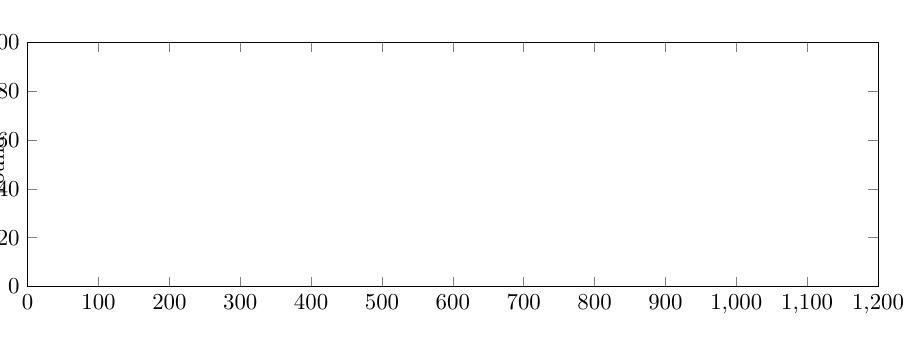
\begin{tikzpicture}[xscale=0.825, yscale=0.825, trim axis left, trim axis right]
			\begin{axis}[
				%xlabel={relative LBA},
				ylabel style={align=center},
				ylabel={(a) \ext\\round\vspace*{-1.5em}},
				xmin=0,
				xmax=1200,
				ymin=0,
				ymax=100,
				width=1.21\columnwidth,
				height=0.44\linewidth,
				]
				\addnewlayoutplot{ext4}{0}
				\addnewlayoutplot{ext4}{10}
				\addnewlayoutplot{ext4}{20}
				\addnewlayoutplot{ext4}{30}
				\addnewlayoutplot{ext4}{40}
				\addnewlayoutplot{ext4}{50}
				\addnewlayoutplot{ext4}{60}
				\addnewlayoutplot{ext4}{70}
				\addnewlayoutplot{ext4}{80}
				\addnewlayoutplot{ext4}{90}
				\addnewlayoutplot{ext4}{100}
			\end{axis}
		\end{tikzpicture}
		%\caption{\ext}
	\end{subfigure}\\
%\end{figure*}
%\begin{figure*}[t]
	\begin{subfigure}{\columnwidth}
		\centering
		\tikzsetnextfilename{layout-intra_btrfs}
		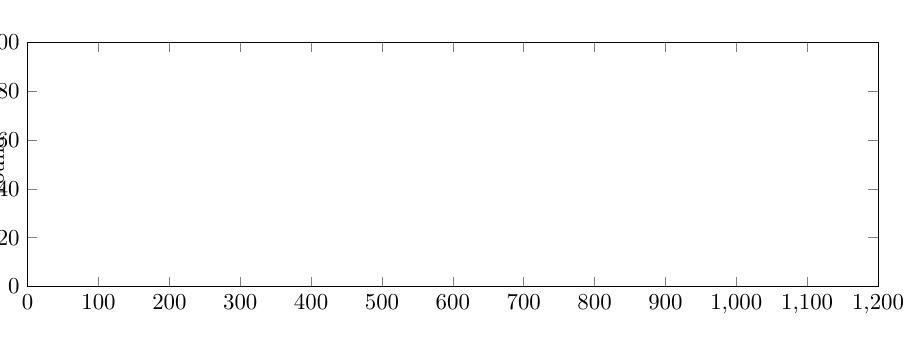
\begin{tikzpicture}[xscale=0.825, yscale=0.825, trim axis left, trim axis right]
			\begin{axis}[
				%xlabel={relative LBA},
				ylabel style={align=center},
				ylabel={(b) \btrfs\\round\vspace*{-1.5em}},
				xmin=0,
				xmax=1200,
				ymin=0,
				ymax=100,
				width=1.21\columnwidth,
				height=0.44\linewidth,
				]
				\addnewlayoutplot{btrfs}{0}
				\addnewlayoutplot{btrfs}{10}
				\addnewlayoutplot{btrfs}{20}
				\addnewlayoutplot{btrfs}{30}
				\addnewlayoutplot{btrfs}{40}
				\addnewlayoutplot{btrfs}{50}
				\addnewlayoutplot{btrfs}{60}
				\addnewlayoutplot{btrfs}{70}
				\addnewlayoutplot{btrfs}{80}
				\addnewlayoutplot{btrfs}{90}
				\addnewlayoutplot{btrfs}{100}
			\end{axis}
		\end{tikzpicture}
		%\caption{\btrfs}
	\end{subfigure}\\
%\end{figure*}
%\begin{figure*}[t]
%{ \centering
	\begin{subfigure}{\columnwidth}
		\centering
		\tikzsetnextfilename{layout-intra_xfs}
		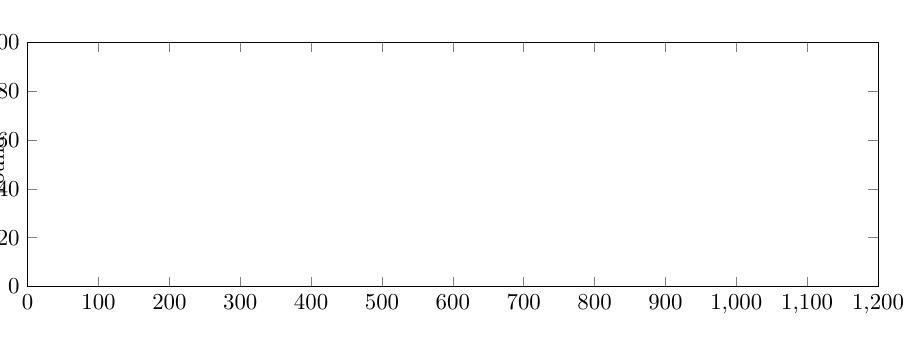
\begin{tikzpicture}[xscale=0.825, yscale=0.825, trim axis left, trim axis right]
			\begin{axis}[
				%xlabel={relative LBA},
				ylabel style={align=center},
				ylabel={(c) \xfs\\round\vspace*{-1.5em}},
				xmin=0,
				xmax=1200,
				ymin=0,
				ymax=100,
				width=1.21\columnwidth,
				height=0.44\linewidth,
				]
				\addnewlayoutplot{xfs}{0}
				\addnewlayoutplot{xfs}{10}
				\addnewlayoutplot{xfs}{20}
				\addnewlayoutplot{xfs}{30}
				\addnewlayoutplot{xfs}{40}
				\addnewlayoutplot{xfs}{50}
				\addnewlayoutplot{xfs}{60}
				\addnewlayoutplot{xfs}{70}
				\addnewlayoutplot{xfs}{80}
				\addnewlayoutplot{xfs}{90}
				\addnewlayoutplot{xfs}{100}
			\end{axis}
		\end{tikzpicture}
		%\caption{\xfs}
	\end{subfigure}\\
%\end{figure*}
%\begin{figure*}[t]
%{ \centering
	\begin{subfigure}{\columnwidth}
		\centering
		\tikzsetnextfilename{layout-intra_zfs}
		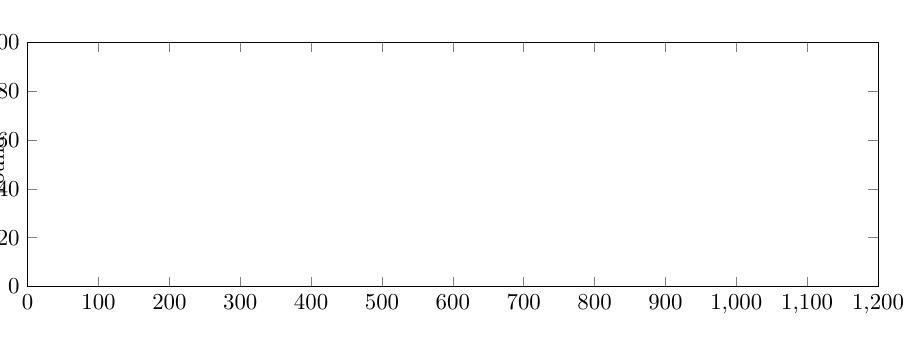
\begin{tikzpicture}[xscale=0.825, yscale=0.825, trim axis left, trim axis right]
			\begin{axis}[
				%xlabel={relative LBA},
				ylabel style={align=center},
				ylabel={(d) \zfs\\round\vspace*{-1.5em}},
				xmin=0,
				xmax=1200,
				ymin=0,
				ymax=100,
				width=1.21\columnwidth,
				height=0.44\linewidth,
				]
				\addnewlayoutplot{zfs}{0}
				\addnewlayoutplot{zfs}{10}
				\addnewlayoutplot{zfs}{20}
				\addnewlayoutplot{zfs}{30}
				\addnewlayoutplot{zfs}{40}
				\addnewlayoutplot{zfs}{50}
				\addnewlayoutplot{zfs}{60}
				\addnewlayoutplot{zfs}{70}
				\addnewlayoutplot{zfs}{80}
				\addnewlayoutplot{zfs}{90}
				\addnewlayoutplot{zfs}{100}
			\end{axis}
		\end{tikzpicture}
		%\caption{\zfs}
	\end{subfigure}\\
%\end{figure*}
%\begin{figure*}[t]
%{ \centering
	\begin{subfigure}{\columnwidth}
		\centering
		\tikzsetnextfilename{layout-intra_f2fs}
		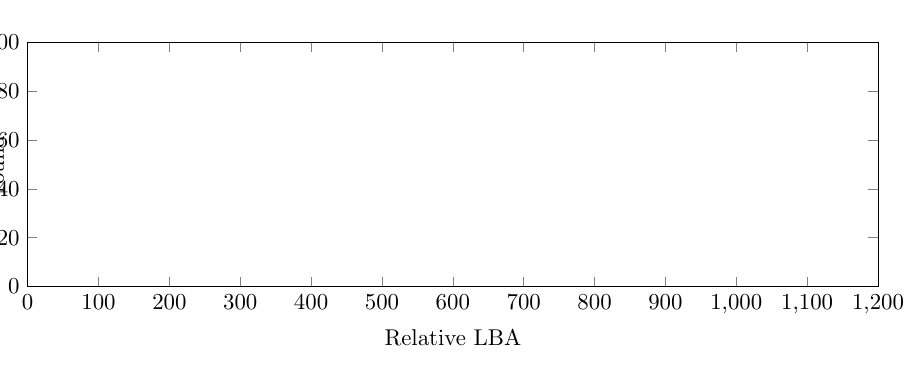
\begin{tikzpicture}[xscale=0.825, yscale=0.825, trim axis left, trim axis right]
			\begin{axis}[
				xlabel={Relative LBA},
				ylabel style={align=center},
				ylabel={(e) \ftwofs\\round\vspace*{-1.5em}},
				xmin=0,
				xmax=1200,
				ymin=0,
				ymax=100,
				width=1.21\columnwidth,
				height=0.44\linewidth,
				]
				\addnewlayoutplot{f2fs}{0}
				\addnewlayoutplot{f2fs}{10}
				\addnewlayoutplot{f2fs}{20}
				\addnewlayoutplot{f2fs}{30}
				\addnewlayoutplot{f2fs}{40}
				\addnewlayoutplot{f2fs}{50}
				\addnewlayoutplot{f2fs}{60}
				\addnewlayoutplot{f2fs}{70}
				\addnewlayoutplot{f2fs}{80}
				\addnewlayoutplot{f2fs}{90}
				\addnewlayoutplot{f2fs}{100}
			\end{axis}
		\end{tikzpicture}
		%\caption{\ftwofs}
	\end{subfigure}
	\caption{\label{fig:mb-intra-layout}Intrafile benchmark layout visualization.  Each color represents blocks of a file.  The x-axis is the logical block address (LBA) of the file block relative to the first LBA of any file block, and y-axis is the round of the experiment.  Rectangle sizes indicate contiguous placement, where larger is better. The brown regions with vertical lines indicate interleaved blocks of all 10 files. Some blocks are not shown for \ext, \xfs and \zfs.}}
\end{figure}


Because of the small amount of data and number of files involved in this
microbenchmark, we can visualize the layout of the various file systems, shown
in \cref{fig:mb-intra-layout}. Each block of a file is represented by a
small vertical bar, and each bar is colored uniquely to one of the ten files.
Contiguous regions form a colored rectangle.  The visualization suggests, for
example, that \ext both tries to keep files and eventually larger file
fragments sequential, whereas \btrfs and \ftwofs interleave the round robin
chunks on the end of the sequential data. This interleaving can help explain
why \btrfs and \ftwofs perform the way they do: the interleaved sections must
be read through in full each time a file is requested, which by the end of the
test takes roughly 10 times as long. \ext and \xfs manage to keep the files in
larger extents, although the extents get smaller as the test progresses, and,
by the end of the benchmark, these file systems also have chunks of interleaved
data; this is why \ext and \xfs's  dynamic layout scores decline.  \zfs keeps
the files in multiple chunks through the test; in doing so it sacrifices some
performance in all states, but does not degrade.

Unfortunately, this sort of visualization doesn't work for \betrfs, because
this small amount of data fits entirely in a leaf.  Thus, \betrfs will read all
this data into memory in one sequential read. This results is some read
amplification, but, on an HDD, only one seek.

% interfile microbenchmark (degrees of random order copy)

\newcommand{\addsfplot}[2]
{
	\pgfplotstableread{fsa-data/camera_ready_microbenchmarks/inter_#2.csv}\thistable
	\addplot[color=\pgfkeysvalueof{/fs-colors/#1}, style=\pgfkeysvalueof{/agedness-styles/aged}, line width=0.75pt, mark=\pgfkeysvalueof{/fs-marks/#1}, mark repeat=5] table[x=round, y=#1_time] \thistable;
	\addlegendentry{\pgfkeysvalueof{/fs-names/#1}}
}

\newcommand{\addsflayoutplot}[2] % \addsfplot{fs}{hdd/ssd/ssd_raoff}
{
  \pgfplotstableread{fsa-data/camera_ready_microbenchmarks/inter_#2.csv}\thistable
  \addplot[color=\pgfkeysvalueof{/fs-colors/#1}, style=\pgfkeysvalueof{/agedness-styles/aged}, line width=0.75pt, mark=\pgfkeysvalueof{/fs-marks/#1}, mark repeat=5]
  table[x=round, y=#1_layout] \thistable;
  \addlegendentry{\pgfkeysvalueof{/fs-names/#1}}
}

\newcommandx{\startsfplot}[2] %\startsfplot{hdd/ssd/ssd_raoff}{maxy}
{
  \begin{tikzpicture}
    \begin{axis}[
      width=\hsize,
      height=0.28\textheight,
      % scale only axis,
      % title=Insertion per second against Load Factor, 
      ylabel style={at={(axis description cs:0.075,0.5)},anchor=south},
	  xlabel={Percentage of files copied out-of-order}, 
      ylabel={Grep cost (sec/GiB)}, 
      xmin=0,
      xmax=100, 
      ymin=0,  
      ymax=#2,
      % xtick={0,20,40,60,80,100},
      % ytick={0,5,10,15,20,25,30,35,40,45,50},
      grid=major, 
      scaled x ticks=false,
      scaled y ticks=false,
      legend columns=6,
      legend cell align=center,
      legend pos=north west,
      legend to name=sfplotslegend_#1,
      %transpose legend,
      ]
    }

\NewEnviron{sfplot}{\expandafter\startsfplot\BODY
\end{axis}
\end{tikzpicture}
}

% args are: hardware 
\newcommandx{\startsflayoutplot}[1]
{
  \begin{tikzpicture}
    \begin{axis}[
      width=\hsize,
      height=0.28\textheight,
      % scale only axis,
      % title=Insertion per second against Load Factor, 
      ylabel style={at={(axis description cs:0.075,0.5)},anchor=south},
      xlabel={Percentage of files copied out-of-order}, 
      ylabel={Dynamic layout score}, 
      xmin=0,
      xmax=100, 
      ymin=0, 
      ymax=1, 
      % xtick={0,20,40,60,80,100},
      % ytick={0,5,10,15,20,25,30,35,40,45,50},
      grid=major, 
      scaled x ticks=false,
      scaled y ticks=false,
      legend columns=6,
      legend cell align=center,
      legend pos=north west,
      legend to name=sflayoutplotslegend_#1,
      %transpose legend,
      ]
    }

\NewEnviron{sflayoutplot}{\expandafter\startsflayoutplot\BODY
\end{axis}
\end{tikzpicture}
}

\newcommand{\sfplotsubcaption}[1]{\label{subfig:sf:#1} Recursive grep cost: \pgfkeysvalueof{/hardware-names/#1} (Lower is better).}
\newcommand{\sflayoutplotsubcaption}[1]{\label{subfig:sfl:#1} Dynamic layout score (higher is better).}

\begin{figure}
  {\centering
    ~\ref{sfplotslegend_hdd}~\\
	\begin{subfigure}{\columnwidth}\label{subfig:sfhdd}
      \centering
	  \tikzsetnextfilename{micro-inter_hdd}
      \begin{sfplot}{hdd}{1000}
        \addsfplot{betrfs}{hdd}
        \addsfplot{btrfs}{hdd}
        \addsfplot{ext4}{hdd}
        \addsfplot{f2fs}{hdd}
        \addsfplot{xfs}{hdd}
        \addsfplot{zfs}{hdd}
      \end{sfplot}
      \caption{\sfplotsubcaption{hdd}}
	\end{subfigure}\\
    \begin{subfigure}{\columnwidth}\label{subfig:sfssd}
      \centering
      \tikzsetnextfilename{micro-inter_ssd}
      \begin{sfplot}{ssd}{100}
        \addsfplot{betrfs}{ssd}
        \addsfplot{btrfs}{ssd}
        \addsfplot{ext4}{ssd}
		\addsfplot{f2fs}{ssd}
        \addsfplot{xfs}{ssd}
        \addsfplot{zfs}{ssd}
      \end{sfplot}
      \caption{\sfplotsubcaption{ssd}}
    \end{subfigure}\\
     \begin{subfigure}{\columnwidth} \label{subfig:sflayout}
       \centering
		 \tikzsetnextfilename{micro-inter_layout}
       \begin{sflayoutplot}{hdd}
         \addsflayoutplot{betrfs}{hdd}
         \addsflayoutplot{btrfs}{hdd}
         \addsflayoutplot{ext4}{hdd}
         \addsflayoutplot{f2fs}{hdd}
         \addsflayoutplot{xfs}{hdd}
         \addsflayoutplot{zfs}{hdd}
       \end{sflayoutplot}
       \caption{\sflayoutplotsubcaption{ssd}}
     \end{subfigure}
    \caption{\label{fig:micro:inter} Interfile benchmark: The TensorFlow github repository with all files replaced by 4KiB random data and copied in varying degrees of order. Dynamic layout scores again are predictive of recursive grep test performance. }
  }
\end{figure}



\paragraph{Interfile Fragmentation.}\label{sec:interfile} Many workloads read
multiple files with some logical relationship, and frequently those files are
placed in the same directory. Interfile fragmentation occurs when files which
are related---in this case by being close together in the directory tree---are not
collocated in the LBA space.

We present a microbenchmark to measure the impact of namespace creation order
on interfile locality. It takes a given ``real-life'' file structure, in this
case the Tensorflow repository obtained from \texttt{github.com}, and replaces
each of the files by 4KiB of random data. This gives us a ``natural'' directory
structure, but isolates the effect of file ordering without the influence of
intrafile layout. The benchmark creates a sorted list of the files as well as
two random permutations of that list. On each round of the test, the benchmark
copies all of the files, creating directories as needed with {\tt cp
--parents}.  However, on the $n$th round, it swaps the order in which the first
$n\%$ of files appearing in the random permutations are copied. Thus, the first
round will be an in-order copy, and subsequent rounds will be copied in a
progressively more random order until the last round is a fully random-order
copy.

The results of this test are shown \cref{fig:micro:inter}.  On hard
drive, all the file systems except \betrfs and \xfs show a precipitous
performance decline even if only a small percentage of the files are copied out
of order. \ftwofs's performance is poor enough to be out of scale for this
figure, but it ends up taking over 4000 seconds per GiB at round 100; this is
not entirely unexpected as it is not designed to be used on hard drive. \xfs is
somewhat more stable, although it is 13-35 times slower than drive bandwidth
throughout the test, even on an in-order copy.  \betrfs consistently performs
around 1/3 of bandwidth, which by the end of the test is 10 times faster than
\xfs, and 25 times faster than the other file systems. The dynamic layout
scores are moderately correlated with this performance ($-0.57$).

On SSD, half the file systems perform stably throughout the test with varying
degrees of performance. The other half have a very sharp slowdown between the
in-order state and the 10\% out-of-order state. These two modes are reflected
in their dynamic layout scores as well. While \ext and \zfs are stable, their
performance is worse than the best cases of several other file systems.
\betrfs is the only file system with stable fast performance; it is faster in
every round than any other file system even in their best case: the in-order
copy. In this cases the performance strongly correlates with the dynamic layout
score ($-0.83$).

\section{Application Level Read-Aging: Git}\label{sec:fsa-git}

To measure aging in the ``real-world,'' we create a workload designed to
simulate a developer using git to work on a collaborative project.

Git is a distributed version control system that enables collaborating
developers to synchronize their source code changes.  Git users \defn{pull}
changes from other developers, which then get merged with their own changes.
In a typical workload, a Git user may perform pulls multiple times per day over
several years in a long-running project.  Git can synchronize all types of file
system changes, so performing a Git pull may result in the creation of new
source files, deletion of old files, file renames, and file modifications.  Git
also maintains its own internal data structures, which it updates during pulls.
Thus, Git performs many operations which are similar to those shown in
\secref{microbenchmarks} that cause file system aging.

We present a git benchmark that performs 10,000 pulls from the Linux git repository, starting
from the initial commit. After every 100 pulls, the benchmark performs a recursive grep
test and computes the file system's dynamic layout score.
This score is compared to the same contents copied to a freshly formatted partition.
%\figref{git-20gb} shows the results
%of the grep tests on both hard disk and SSD.

% \subsection{HDD} The above microbenchmarks highlight the compromises that
% traditional file systems must make when files are manipulated, and we now
% demonstrate this effect under a ``realistic workload.'' Git is a \fixme{blah
% blah about what git is}. From the perspective of the file system, much of a
% programmer's workload consists of fetching changes to the source code from a
% remote repository and merging them into the local source. Thus we use this
% process to simulate such a workload.

% The data on the file system consists of a git repository into which we pull successive commits from the linux source code repository, starting with the initial one. The first 10,000 commits reachable from the current HEAD (as of whenever) are used in commit time order, and are pulled via the command \texttt{git pull \$remote \$commit}, where the remote repository has the config option \texttt{uploadpack.allowReachableSHA1InWant} enabled to allow fetching of arbitrary commits. After initializing the repository with the first commit, and after every thousand commits, we perform a \texttt{grep} test as above.

% As git pulls commits, files are created, deleted and changed in the target file system, and we expect that over time the file system will respond to the aging stress this creates. \fixme{maybe some discussion of the sorts of operations that git does?} The results are shown in figure \fixme{***}.

\input{git-main-plots}

\fixmeac{remember to update corr coeffs with data}

On a hard disk (Figure~\ref{fig:git:results:hdd:20gb:on}), there is a clear
aging trend in all file systems except \betrfs.  By the end of the experiment,
all the file systems except \betrfs show performance drops under aging on the
order of at least 3x and as much as 15x relative to their unaged versions. All
are at least 15x worse than \betrfs. In all of the experiments in this section,
\ftwofs ages considerably more than all other file systems, commensurate with
significantly lower layout scores than the other file systems---indicating less
effective locality in data placement. The overall correlation between grep
performance and dynamic layout score is moderate, at $-0.41$. 

On an SSD (Figure~\ref{fig:git:results:ssd:20gb:on}), \btrfs and \xfs show
clear signs of aging, although they converge to a fully aged configuration
after only about 1,000 pulls. While the effect is not as drastic as on HDD, in
all the traditional file systems we see slowdowns of 2x-4x over \betrfs, which
does not slow down.  In fact, aged \betrfs on the HDD outperforms all the other
aged file systems on an SSD, and is close even when they are unaged. Again,
this performance decline is strongly correlated ($-0.79$) with the dynamic
layout scores.

The aged and unaged performance of \ext and \zfs are comparable, and slower
than several other file systems.  We believe this is because the average file
size decreases over the course of the test, and these file systems are not as
well-tuned for small files.  To test this hypothesis, we constructed
synthetic workloads similar to the interfile fragmentation microbenchmark
(\secref{microbenchmarks}), but varied the file size (in the microbenchmark it
was uniformly 4KB). 
Figure~\ref{fig:git:filesize} shows both the measured, average file
size of the git workload (one point is one pull), and the microbenchmark.
Overall, there is a clear relationship between the average file size and grep
cost. 
%, and the grep cost increases steeply when the average file is
%smaller than 16 KiB.

\input{git-filesize-plots}

The zig-zag pattern in the graphs is created by an automatic garbage collection
process in Git. Once a certain number of ``loose objects'' are created (in git
terminology), many of them are collected and compressed into a ``pack.'' At the
file system level, this corresponds to merging numerous small files into a
single large file.  According to the Git manual, this process is designed to
``reduce disk space and increase performance,'' so this is an example of an
application-level attempt to mitigate file system aging. If we turn off the git
garbage collection, as show in Figures~\ref{fig:git:results:hdd:20gb:off},
\ref{fig:git:results:ssd:20gb:off} and \ref{subfig:git:layout:20gb:off}, the
effect of aging is even more pronounced, and the zig-zags essentially disappear.

%\fixmeac{Kill this paragraph or add HDD results description?}
On both the HDD and SSD, the same patterns emerge as with garbage collection
on, but exacerbated: \ftwofs aging is by far the most extreme.  \zfs ages
considerably on the HDD, but not on the SSD.  \zfs on SSD and \ext perform
worse than the other file systems (except \ftwofs aged), but do not age
particularly.  \xfs and \btrfs both aged significantly, around 2x each, and
\betrfs has strong, level performance in both states. This performance
correlates with dynamic layout score both on SSD ($-0.78$) and moderately so on
HDD ($-0.54$).

We note that this analysis, both of the microbenchmarks and of the git
workload, runs counter to the commonly held belief that locality is solely a
hard drive issue. While the random read performance of solid state drives does
somewhat mitigate the aging effects, aging clearly has a major
performance impact.

%\fixmedp{This is a good start on measuring what is going on.  I'd like to better understand the file placement heuristics on ext4 and btrfs---why do they make different choices?  Maybe even see a different example directory layout + physical placement}
%\fixmeac{Reminder to add a deferred allocation comment here somewhere}

\tightpara{Git Workload with Warm Cache.}
The tests we have presented so far have all been performed with a cold cache,
so that they more or less directly test the performance of the file systems'
on-disk layout under various aging conditions. In practice, however, some data
will be in cache, and so it is natural to ask how much the layout choices that
the file system makes will affect the overall performance with a warm cache.

We evaluate the sensitivity of the git workloads to varying amounts of system
RAM.  We use the same procedure as above, except that we do not flush any
caches or remount the hard drive between iterations.  This test is performed on
a hard drive with git garbage collection off.  The size of the data on disk is
initially about 280MiB and grows throughout the test to approximately 1GiB.

\input{git-wc-plots}

The results are summarized in \figref{git:warmcache}. We present data for \ext
and \ftwofs; the results for \btrfs, \xfs and \zfs are similar. \betrfs is a
research prototype and unstable under memory pressure; although we plan to fix
these issues in the future, we omit this comparison.
% low-memory conditions, 
%in this test for reasons unrelated to disk layout.  Although we plan to fix
%this issue in the future, we omit the \betrfs comparison in the interest of
%clarity.  under memory pressure, for so we omit this data in the interest of
%clarity.  Unfortunately \betrfs is a research prototype and does not behave
%well in low memory conditions. As such we are unable to present its results
%here outright.

In general, when the caches are warm and there is sufficient memory to keep all
the data in cache, then the read is very fast. However, as soon as there is no
longer sufficient memory, the performance of the aged file system with a warm
cache is generally worse than unaged with a cold cache.  In general, unless all
data fits into DRAM, a good layout matters more than a having a warm cache.
%good layout and cold cache---Cold Cache Unaged and \betrfs Cold Cache lines in
%the figures---quickly outperforms the aged layout when all data doesn't fit in
%DRAM, even with a warm cache.
  
\tightpara{Btrfs Node-Size Trade-Off.}
\Btrfs allows users to specify the node size of its metadata B-tree 
at creation time. Because small files are stored in the metadata
B-tree, a larger node size results in a less fragmented file system, at a cost of
more expensive metadata updates.
%One of the design considerations we put forth in \secref{model} is that, in
%general, the use of larger block sizes would lead to reduced aging. However,
%doing so naively leads to write-amplification as the larger blocks are still
%written even for small modifications. We demonstrate this using the above git
%workload on \btrfs, a B-Tree-based file system. Here block size corresponds to
%the size of the nodes of the tree, which \btrfs allows us to configure when
%formatting.

We present the git test with a 4KiB node size, the default setting, as well as 8KiB,
16KiB, 32KiB, and 64KiB (the maximum).  
\figref{btrfsGrepTime:results:hdd:20gb:off} shows similar
performance graphs to \figref{git-20gb}, one line for each node size.  The 4KiB
node size has the worst read performance by the end of the test, and the
performance consistently improves as we increase the node size all the way to
64KiB.  \figref{btrfsBlocksWritten:results:hdd:20gb:off} plots the number
of 4KiB blocks written to disk between each test (within the 100 pulls).  As
expected, the 64KiB node size writes the maximum number of blocks and the 4KiB
node writes the least.  We thus demonstrate---as predicted by our model---that
aging is reduced by a larger block size, but at the cost of write-amplification.

\input{git-node_size-plots}

\section{Application Level Aging: Mail Server}\label{sec:fsa-mailserver} In
addition to the git workload, we evaluate aging with the Dovecot email server.
Dovecot is configured with the Maildir backend, which stores each message in a
file, and each inbox in a directory.  We simulate 2 users, each having 80
mailboxes, receiving new email, deleting old emails, and searching through their
mailboxes. 

A cycle or ``day'' for the mailserver comprises 8,000 operations, where each
operation is equally likely to be an insert or a delete, corresponding to
receiving a new email or deleting an old one. Each email is a string of random
characters, the length of which is uniformly distributed over the range [1,
32K]. Each mailbox is initialized with 1,000 messages, and, because inserts and
deletes are balanced, mailbox size tends to stay around 1,000.  We simulate the
mailserver for 100 cycles and after each cycle we perform a recursive grep for
a random string. As in our git benchmarks, we then copy the partition to a
freshly formatted file system, and run a recursive grep.

\cref{fig:mailserver} shows the read costs in seconds per GiB of the grep test
on hard disk.  Although the unaged versions of all file systems show consistent
performance over the life of the benchmark, the aged versions of \ext, \btrfs,
\xfs and \zfs all show significant degradation over time. In particular, aged
\ext performance degrades by 4.4$\times$, and is 28$\times$ slower than aged
\betrfs.  \xfs slows down by a factor of 7 and \btrfs, by a factor of 30. \zfs
slows down drastically, taking about 20 minutes per GiB by cycle 20.  However,
the aged version of \betrfs does not slow down. As with the other HDD
experiments, dynamic layout score is moderately correlated ($-0.63$) with grep
cost.

%
% File parsing definitions
%
\newcommand{\mailserverDataDir}{fsa-data/mailserver_aging}
% Args: hardware, partition-size, file-system
\newcommand{\mailserverDataFileName}[3]{\mailserverDataDir/mailserver_#3_#1_#2.csv}
\newcommand{\mailserverOperationCountColumn}{pulls_performed}
\newcommand{\mailserverFSSizeColumn}{filesystem_size}
\newcommand{\mailserverLayout}[1]{#1_layout_score}

% construct a table with the reference FS sizes from ext4 on hdd
\pgfplotstableread{\mailserverDataFileName{hdd}{20gb}{ext4}}\extfourmsdata

% args are: FS agedness hardware partition-size
\newcommand{\addmailserverplot}[4]
{
  \pgfplotstableread{\mailserverDataFileName{#3}{#4}{#1}}\thistable
  \pgfplotstablecreatecol[copy column from table={\extfourmsdata}{\mailserverFSSizeColumn}]{ext4_fs_size}{\thistable}
  \addplot[color=\pgfkeysvalueof{/fs-colors/#1}, style=\pgfkeysvalueof{/agedness-styles/#2}, line width=0.75pt, mark=\pgfkeysvalueof{/fs-marks/#1}, mark repeat=5] 
  table[x=\mailserverOperationCountColumn, y expr=\thisrow{\pgfkeysvalueof{/agedness-columns/#2}} / \thisrow{ext4_fs_size} * 1048576] \thistable;
  %\addfsplot{#1}{#2}{\pullCountColumn}{\thisrow{\pgfkeysvalueof{/agedness-columns/#2}} / \expandafter\thisrow{ext4_fs_size} * 1000000}{\thistable}
  %\addlegendentry{\pgfkeysvalueof{/fs-names/#1} \pgfkeysvalueof{/agedness-names/#2}}
}

% args are: hardware partition-size
\newcommandx{\startmsplot}[2]
{
   \begin{tikzpicture}
      \begin{axis}[
            width=\hsize,
            height=0.45\textheight,
      % scale only axis,
      % title=Insertion per second against Load Factor, 
      xlabel={Operations performed}, 
      ylabel={Grep cost (sec/GiB)}, 
      xmin=0,
      xmax=100, 
      ymin=0, 
      % ymax=50, 
      % xtick={0,20,40,60,80,100},
      % ytick={0,5,10,15,20,25,30,35,40,45,50},
      yticklabel style={rotate=90, anchor=south},
      grid=major, 
      scaled x ticks=false,
      scaled y ticks=false,
         legend entries = { \btrfs, \betrfs, \ext, \ftwofs, \xfs, \zfs, aged, unaged},
      legend columns=8,
      legend cell align=center,
      legend pos=north west,
      legend to name=mailserverplotslegend_#1_#2,
      ]
  	\addlegendimage{\pgfkeysvalueof{/fs-colors/btrfs}, mark=\pgfkeysvalueof{/fs-marks/btrfs}}
  	\addlegendimage{\pgfkeysvalueof{/fs-colors/betrfs}, mark=\pgfkeysvalueof{/fs-marks/betrfs}}
  	\addlegendimage{\pgfkeysvalueof{/fs-colors/ext4}, mark=\pgfkeysvalueof{/fs-marks/ext4}}
  	\addlegendimage{\pgfkeysvalueof{/fs-colors/f2fs}, mark=\pgfkeysvalueof{/fs-marks/f2fs}}
  	\addlegendimage{\pgfkeysvalueof{/fs-colors/xfs}, mark=\pgfkeysvalueof{/fs-marks/xfs}}
  	\addlegendimage{\pgfkeysvalueof{/fs-colors/zfs}, mark=\pgfkeysvalueof{/fs-marks/zfs}}
    %\pgfplotsinvokeforeach{btrfs, betrfs, ext4, f2fs, xfs, zfs} {
  	%  \addlegendimage{\pgfkeysvalueof{/fs-colors/#1}, mark=\pgfkeysvalueof{/fs-marks/#1}}
    %}
  	\addlegendimage{mark=\pgfkeysvalueof{/fs-marks/ext4}, color=\pgfkeysvalueof{/fs-colors/ext4},  style=\pgfkeysvalueof{/agedness-styles/aged}}
  	\addlegendimage{mark=\pgfkeysvalueof{/fs-marks/ext4}, color=\pgfkeysvalueof{/fs-colors/ext4}, style=\pgfkeysvalueof{/agedness-styles/clean}}
}

\NewEnviron{msplot}{\expandafter\startmsplot\BODY
\end{axis}
\end{tikzpicture}
}

\newcommand{\msplotsubcaption}[2]{\label{fig:ms:results:#1:#2} Results: \pgfkeysvalueof{/hardware-names/#1}, \pgfkeysvalueof{/partition-size-names/#2} partition}

% fs agedness hardware partition-size
\newcommand{\addmslayoutplot}[4]
{
  \pgfplotstableread{\mailserverDataFileName{#3}{#4}{#1}}\thistable
  \addplot[color=\pgfkeysvalueof{/fs-colors/#1}, style=\pgfkeysvalueof{/agedness-styles/#2}, line width=0.75pt, mark=\pgfkeysvalueof{/fs-marks/#1}, mark repeat=5] 
  table[x=\mailserverOperationCountColumn, y=\mailserverLayout{#2}] \thistable;
  %\addfsplot{#1}{#2}{\pullCountColumn}{\thisrow{\pgfkeysvalueof{/agedness-columns/#2}} / \expandafter\thisrow{ext4_fs_size} * 1000000}{\thistable}
  %\addlegendentry{\pgfkeysvalueof{/fs-names/#1} \pgfkeysvalueof{/agedness-names/#2}}
}

% args are: hardware partition-size
\newcommandx{\startmslayoutplot}[2]
{
	\begin{tikzpicture}
    \begin{axis}[
      width=\hsize,
      height=0.45\textheight,
      % scale only axis,
      % title=Insertion per second against Load Factor, 
      xlabel={Operations performed}, 
      ylabel={Dynamic layout score}, 
      xmin=0,
      xmax=100, 
      ymin=0, 
      % ymax=50, 
      % xtick={0,20,40,60,80,100},
      % ytick={0,5,10,15,20,25,30,35,40,45,50},
      yticklabel style={rotate=90, anchor=south},
      grid=major, 
      scaled x ticks=false,
      scaled y ticks=false,
      ]
}

\NewEnviron{mslayoutplot}{\expandafter\startmslayoutplot\BODY
\end{axis}
\end{tikzpicture}
}
%
% mailserver figures
%

\begin{figure}
  {\centering
   \ref{mailserverplotslegend_hdd_20gb}\\
    \begin{subfigure}{\columnwidth}
      \centering
	  \tikzsetnextfilename{mailserver-hdd}
      \begin{msplot}{hdd}{20gb}
        \addmailserverplot{betrfs}{clean}{hdd}{20gb}
        \addmailserverplot{betrfs}{aged}{hdd}{20gb}
        \addmailserverplot{btrfs}{clean}{hdd}{20gb}
        \addmailserverplot{btrfs}{aged}{hdd}{20gb}
        \addmailserverplot{ext4}{clean}{hdd}{20gb}
        \addmailserverplot{ext4}{aged}{hdd}{20gb}
        \addmailserverplot{f2fs}{clean}{hdd}{20gb}
        \addmailserverplot{f2fs}{aged}{hdd}{20gb}
        \addmailserverplot{xfs}{clean}{hdd}{20gb}
        \addmailserverplot{xfs}{aged}{hdd}{20gb}
        \addmailserverplot{zfs}{clean}{hdd}{20gb}
        \addmailserverplot{zfs}{aged}{hdd}{20gb}
      \end{msplot}
		\caption{Grep cost during mailserver workload (lower is better).}
    \end{subfigure}
    \begin{subfigure}{\columnwidth}
      \centering
	  \tikzsetnextfilename{mailserver-layout}
      \begin{mslayoutplot}{hdd}{20gb}
        \addmslayoutplot{betrfs}{clean}{hdd}{20gb}
        \addmslayoutplot{betrfs}{aged}{hdd}{20gb}
        \addmslayoutplot{btrfs}{clean}{hdd}{20gb}
        \addmslayoutplot{btrfs}{aged}{hdd}{20gb}
        \addmslayoutplot{ext4}{clean}{hdd}{20gb}
        \addmslayoutplot{ext4}{aged}{hdd}{20gb}
        \addmslayoutplot{f2fs}{clean}{hdd}{20gb}
        \addmslayoutplot{f2fs}{aged}{hdd}{20gb}
        \addmslayoutplot{xfs}{clean}{hdd}{20gb}
        \addmslayoutplot{xfs}{aged}{hdd}{20gb}
        \addmslayoutplot{zfs}{clean}{hdd}{20gb}
        \addmslayoutplot{zfs}{aged}{hdd}{20gb}
      \end{mslayoutplot}
		\caption{Mailserver layout (higher is better).}
    \end{subfigure}
    \caption{\label{fig:mailserver} Mailserver performance and layout scores.}
  }
\end{figure}

\section{Conclusion}\label{sec:fsa-conclusion}

The experiments above suggest that conventional wisdom on fragmentation, aging,
allocation and file systems is inadequate in several ways.

First, while it may seem intuitive to write data as few times as possible,
writing data only once creates a tension between the logical ordering
of the file system's current state and the potential to make modifications
without disrupting the future order. Rewriting data
multiple times allows the file system to maintain locality.  The overhead
of these multiple writes can be managed by rewriting data in batches, as is done in
write-optimized dictionaries.

% , and the overhead can
% be managed. The point is that not all writes are created equal; a logarithmic
% number of writes with very low write amplification will induce a lower write
% workload than a single write with large write amplification.

For example, in \betrfs, data might be written as many as a
logarithmic number of times, whereas in \ext, it will be written once,
yet \betrfs in general is able to perform as well as or better than an
unaged \ext file system and significantly outperforms aged \ext file
systems.

Second, today's file system heuristics are not able to maintain enough
locality to enable reads to be performed at the disks natural transfer
size.  And since the natural transfer size on a rotating disk is a
function of the seek time and bandwidth, it will tend to increase with
time. Thus we expect this problem to possibly become worse with newer
hardware, not better.

We experimentally confirmed our expectation that non-write-optimized
file systems would age, but we were surprised by how
quickly and dramatically aging impacts performance.
%It was somewhat surprising how quickly they all aged.  
This rapid aging is important: a user's
%(of at least certain workloads)
experience with unaged
file systems is likely so fleeting that they do not notice performance degradation.
Instead, the performance costs of aging
are built into their expectations of file system performance.

% dp: This para really doesn't do it for me
%%% There is quite a lot of future work to perform on aging.  Write
%%% optimization, and specifically \betrfs, appears to avoid aging, as
%%% predicted by our framework and design considerations.  Is there
%%% anything short of wholesale adoption of write optimization that could
%%% be applied to existing file systems to mitigate the effects of aging?
%%% Furthermore, SSDs present further issues, due to their performance
%%% profile and the FTL. Nonetheless, write optimization does generally
%%% improve aged performance on these devices, suggesting that integrating
%%% write-optimized data structures could further improve performance if
%%% they were incorporated to FTL designs.

Finally, because representative aging is a difficult goal, simulating multi-year workloads,
%Because of the perceived difficulty of aging file systems, 
many research 
papers benchmark on unaged file systems.
Our results indicate that it is relatively easy to quickly drive
a file system into an aged state---even if
this state is not precisely the state of the file system after, say, three
years of typical use---and this degraded state can be easily 
measured.

%%%  remark is that the current opinion generally appears to be
%%% that aging a file system is a difficult and elusive goal, since it may
%%% require simulating multi-year workloads. As a
%%% result, %of the perceived level of care required 
%%% many current research papers
%%% routinely benchmark on an unaged file system. 
%%% %We argue that it is
%%% %important to measure the expected state of use, even though precisely
%%% %recreating a specific aged state requires significant effort.  
%%% A key
%%% observation from our experiments, however, is that there is a
%%% precipitous drop from a clean, initial state, to an aged state in
%%% current file systems.  In other words, it is relatively easy to
%%% quickly drive a file system into a significantly aged state, even if
%%% this state is not precisely the state of the file system after three
%%% years of typical use.


%% Local Variables:
%% mode: latex
%% End:


\chapter{Optimal Ball Recycling}
%!TEX root = paper.tex

\section{Introduction}

Balls-and-bins games have been a successful tool for modeling load balancing
problems~\cite{DBLP:journals/tpds/Mitzenmacher01,DBLP:conf/stoc/AdlerCMR95,DBLP:conf/esa/AdlerBS98,DBLP:journals/siamcomp/AzarBKU99,DBLP:conf/random/ColeFMMRSU98,DBLP:conf/stoc/ColeMHMRSSV98,DBLP:journals/rsa/CzumajS01,DBLP:conf/focs/Mitzenmacher96,DBLP:journals/mst/Mitzenmacher99,DBLP:journals/jacm/Vocking03,DBLP:journals/rsa/BringmannSSS16,DBLP:journals/algorithmica/Park17,WestZaWa16,DBLP:journals/talg/Farach-ColtonFM09,DBLP:conf/icalp/ConwayFS18}.
For example, they can be used to study the average and worst-case occupancy of
buckets in a hash table~\cite{DBLP:journals/corr/abs-0901-1155}, the
worst-case load on nodes in a distributed
cluster~\cite{PetrovaOlMa10,DBLP:conf/podc/BerenbrinkFKMNW16} and even the amount
of time customers wait in line at the grocery store~\cite{DBLP:journals/mst/Mitzenmacher99}.  In
all these load-balancing problems, balls-and-bins games are used to study how
to distribute load evenly across the resource being allocated.

In this paper we study a new scenario, which we refer to as the
\defn{ball-recycling game}, defined as follows:
\begin{displayquote}
	Throw $m$ balls into $n$ bins i.i.d.\ according to a given probability
	distribution $\p$.  Then, at each time step, pick a non-empty bin and
	\defn{recycle} its balls: take the balls from the selected bin and re-throw
	them according to $\p$.
\end{displayquote}
We call a bin-picking method a \defn{recycling strategy} and define its
\defn{recycling rate} to be the expected number of balls recycled in the
stationary distribution (when it exists).

The ball-recycling game models \defn{insertion buffers} and \defn{update
buffers}, which are widely used to speed up insertions in databases by batching
updates to blocks on disk. The recycling rate of a recycling strategy
corresponds to the speed-up obtained by an insertion buffer, so the goal
studied in this paper is how to maximize the recycling rate. This relationship
is described in \cref{sec:br-motivation}, and the experiments in
\cref{sec:br-experiments} demonstrate that it holds in practice.

In this paper, we present results for ball recycling for both general $\p$ and
for the special case of uniform $\p$, which we denote by $\uni$.  As we explain
in \cref{sec:br-motivation}, these distributions correspond to update and
insertion buffers, respectively.

We focus on three natural recycling strategies:
\begin{itemize}
\item \FB: A greedy strategy that recycles the bin with the most balls.
\item \RB: A strategy that picks a ball uniformly at random and recycles its
	bin.
\item \GG: A strategy that picks the bins in round-robin fashion; after a bin
	is picked, the next bin picked is its non-empty successor.
\end{itemize}
Let $\halfnormp = (\sum \sqrt{\p_i})^2$  be the half quasi-norm of $\p$.  We
achieve the following result for general $\p$.

\begin{theorem}[\cref{sec:br-nonuniform}]\label{thm:random-opt}
	Consider a ball-recycling game with $m$ balls and $n$ bins, where the balls
	are distributed into the bins i.i.d.\ according to distribution $\p$. Then
	\RB{} is $\Theta(1)$-optimal.

        It achieves recycling rate
	$\mathcal{R}^\textrm{RB}$:
	\begin{enumerate}
		\item If $m \geq n$,
			\[\mathcal{R}^\textrm{RB} = \Theta\left(\frac{m}{\halfnormp}\right).\]
		\item If $m < n$, let $L$ be the $m$ lowest-weight bins, $q = \sum_{\ell\in
			L} p_\ell$, and $\mathcal{R}_L^\textrm{RB}$ be the recycle rate of
			\RB restricted to $L$. Then,
			\[\mathcal{R}^\textrm{RB} =
			\Theta\left(\min\left(\mathcal{R}_L^\textrm{RB}, 1/q\right)\right).\]
	\end{enumerate}
\end{theorem}

In order to establish this result, we first show that no recycling strategy can
achieve a higher recycling rate than $(2m+n)/\halfnormp$.  This directly
establishes optimality when $m = \Omega(n)$. For $m=o(n)$, we show that \RB
performs as well as another strategy, \AE, which takes an optimal strategy on a
subset of high-weight bins and turns it into an optimal strategy on all the
bins.

Interestingly, the greedy strategy \FB is not generally optimal, and in
particular:
\begin{observation}
There are distributions for which \FB is pessimal, that is, it
recycles at most 2 balls per round whereas OPT recycles almost $m$
balls per round.
\end{observation}
For example, consider the \defn{skyscraper distribution}, where $\p_0 =
1-1/n+1/n^2$ and $\p_i = 1/n^2$, for $0<i\leq n-1$.  Suppose that $m=\sqrt{n}$.
Then \FB will pick bin $0$ every time until it has at most one ball, at which
point it will pick another bin, which will almost certainly have $1$ ball in
it.  Thus, the recycling rate of \FB drops below $2$.  Suppose, instead, that
we recycle the least-full non-empty bin.  In this case, every approximately
$\sqrt{n}$ rounds, a ball lands in a low-probability bin and is promptly
returned to bin $0$. Thus, the recycling rate of this strategy is nearly $m$.
Thus, \FB is pessimal for this distribution.

However, the uniform distribution is of particular importance to insertion
buffers for databases based on \btrees{}. This is because (arbitrary) random
\btree{} insertions are nearly uniformly distributed across the leaves of the
\btree{}, as we show in \cref{sec:br-motivation}. On the uniform distribution, \FB
and \GG are optimal even up to lower order terms:

\begin{theorem}[\cref{sec:br-uniform}]\label{thm:fullestbin}
  \FB and \GG are optimal to within an additive constant for the
  ball-recycling game with distribution $\uni$ 
  for any $n$ and $m$.  They each achieve a
  recycling rate of at least $2m/(n+1)$, whereas no recycling strategy can
  achieve a recycling rate greater than $2m/n + 1$.
\end{theorem}

In this case, \RB is only optimal to within a multiplicative constant
in the following range:

\begin{theorem}[\cref{sec:br-uniform}]\label{thm:rbuniform}
	On the uniform distribution $\uni$, for sufficiently large
        $m$, \RB is at least $(1/2+1/(2^3
	3^4))$-optimal and at most $(1-3/1000)$-optimal.
\end{theorem}

Thus, we establish some surprising results: that \FB can perform poorly for
arbitrary $\p$ but is optimal for $\uni$, up to lower-order terms; and that \RB
is asymptotically optimal for any $\p$ and in particular is more than
$1/2$-optimal but not quite optimal for $\uni$.

In \cref{sec:br-experiments}, we present experimental results showing that our
analytical results for the ball recycling problem closely match performance
results in real databases.  We describe the recycling strategies of several
commercial and open-source database systems. In particular we focus on InnoDB,
a \btree{} that uses a variant of \RB.

Our results suggest that \FB or \GG would be a better choice than \RB for
InnoDB. In particular, \GG requires almost no additional bookkeeping, and can
be implemented in InnoDB with a change of only a few lines of code.
With this implementation, we measured a 30\% improvement in its
insertion-buffer flushing rate, which is in line with our theoretical results.

We conclude that ball recycling is a natural hitherto unexplored balls-and-bins
game that closely models a widely deployed method for improving the performance
of databases. Moreover, this is the first application (to our knowledge) of a
balls-and-bins game to the throughput of a system. This is in contrast to past
balls-and-bins analyses, which modeled load balancing and latency.


%%% Local Variables:
%%% mode: latex
%%% TeX-master: "paper.tex"
%%% End:


\bibliographystyle{plainurl}
\bibliography{./bibliography}
\end{document}
